% **************************************************
% Document Class Definition
% **************************************************
\documentclass[%
    paper=A4,               % paper size --> A4 is default in Germany
    twoside=true,           % onesite or twoside printing
    openright,              % doublepage cleaning ends up right side
    parskip=full,           % spacing value / method for paragraphs
    chapterprefix=true,     % prefix for chapter marks
    11pt,                   % font size
    headings=normal,        % size of headings
    bibliography=totoc,     % include bib in toc
    listof=totoc,           % include listof entries in toc
    titlepage=on,           % own page for each title page
    captions=tableabove,    % display table captions above the float env
    draft=false,            % value for draft version
]{scrreprt}%

\usepackage{eucal}
\usepackage{mathptmx}
\usepackage{amssymb}
\usepackage{float}
\usepackage{amsmath}


% **************************************************
% Setup YOUR thesis document in this file !
% **************************************************
% !TEX root = main.tex


% **************************************************
% Files' Character Encoding
% **************************************************
\PassOptionsToPackage{utf8}{inputenc}
\usepackage{inputenc}


% **************************************************
% Information and Commands for Reuse
% **************************************************
\newcommand{\thesisTitle}{Machine Learning For Predictive Maintenance\\A Short Survey}
\newcommand{\thesisName}{Anurose Prakash, Christopher Zinda, Gourav Prakash, Paul Fährmann, Saghar Heidari, Sanjay Gupta, Selami Hoxha, Vinay Kaundinya}
\newcommand{\thesisSubject}{Machine Learning For Predictive Maintenance - A Short Survey}
\newcommand{\thesisDate}{\today}
\newcommand{\thesisVersion}{0.1}

\newcommand{\thesisFirstReviewer}{Prof. Eyke Hüllermeier}
\newcommand{\thesisFirstReviewerUniversity}{\protect{Paderborn University}}
\newcommand{\thesisFirstReviewerDepartment}{Department of Computer Science}

\newcommand{\thesisSecondReviewer}{Tanja Tornede}
\newcommand{\thesisSecondReviewerUniversity}{\protect{Paderborn University}}
\newcommand{\thesisSecondReviewerDepartment}{Department of Computer Science}

\newcommand{\thesisFirstSupervisor}{Prof. Eyke Hüllermeier}
\newcommand{\thesisSecondSupervisor}{Tanja Tornede}

\newcommand{\thesisUniversity}{}
\newcommand{\thesisUniversityDepartment}{Department of Computer Science}
\newcommand{\thesisUniversityInstitute}{Paderborn University}
\newcommand{\thesisUniversityGroup}{Intelligent Systems and Machine Learning}
\newcommand{\thesisUniversityCity}{Paderborn}
\newcommand{\thesisUniversityStreetAddress}{Pohlweg 51}
\newcommand{\thesisUniversityPostalCode}{33098}


% **************************************************
% Debug LaTeX Information
% **************************************************
%\listfiles


% **************************************************
% Load and Configure Packages
% **************************************************
\usepackage[english]{babel} % babel system, adjust the language of the content
\PassOptionsToPackage{% setup clean thesis style
    figuresep=colon,%
    sansserif=false,%
    hangfigurecaption=false,%
    hangsection=true,%
    hangsubsection=true,%
    colorize=full,%
    colortheme=upbisg,%
    bibsys=biber,%
    bibfile=bib-refs,%
    bibstyle=alphabetic,%
    wrapfooter=false,%
}{cleanthesis}
\usepackage{cleanthesis}

\usepackage{mathtools}

\hypersetup{% setup the hyperref-package options
    pdftitle={Machine Learning For Predictive Maintenance - A Short Survey},    %   - title (PDF meta)
    pdfsubject={\thesisSubject},%   - subject (PDF meta)
    pdfauthor={\thesisName},    %   - author (PDF meta)
    plainpages=false,           %   -
    colorlinks=false,           %   - colorize links?
    pdfborder={0 0 0},          %   -
    breaklinks=true,            %   - allow line break inside links
    bookmarksnumbered=true,     %
    bookmarksopen=true          %
}


% **************************************************
% Document CONTENT
% **************************************************
\begin{document}


% --------------------------
% rename document parts
% --------------------------
%\renewcaptionname{ngerman}{\figurename}{Abb.}
%\renewcaptionname{ngerman}{\tablename}{Tab.}
\renewcaptionname{english}{\figurename}{Fig.}
\renewcaptionname{english}{\tablename}{Tab.}

% --------------------------
% Front matter
% --------------------------
\pagenumbering{roman}			% roman page numbing (invisible for empty page style)
\pagestyle{empty}				% no header or footers
% !TEX root = ../main_sys.tex
%
% ------------------------------------  --> cover title page
\begin{titlepage}
	\pdfbookmark[0]{Cover}{Cover}
	\flushright
	\hfill
	\vfill
	{\LARGE\thesisTitle \par}
	\rule[5pt]{\textwidth}{.4pt} \par
	{\Large\thesisName}
	\vfill
	\textit{\large\thesisDate} \\
	% Version: \thesisVersion
\end{titlepage}


% ------------------------------------  --> main title page
\begin{titlepage}
	\pdfbookmark[0]{Titlepage}{Titlepage}
	\tgherosfont

	\begin{figure}
		\begin{minipage}[t]{8.5cm}
			
\includegraphics[height=1.8cm]{gfx/upb_logo}\\
			\textsf{\small{\hspace*{1.3cm}Department of Electrical Engineering,\\
					\hspace*{1.3cm}Computer Science and Mathematics\\
					%		\hspace*{1.3cm}Institute of Computer Science\\
					\hspace*{1.3cm}Warburger Straße 100 \\
					\hspace*{1.3cm}33098 Paderborn
				}}
		\end{minipage}
		\hfill
		\begin{minipage}[t]{4.7cm}
			
\includegraphics[height=1.8cm]{gfx/is-logo-klein}\\
			\textsf{%Institute of Computer Science\\
				\small{Intelligent Systems and Machine Learning}
			}
		\end{minipage}
	\end{figure}

	\centering
	%\textsf{\thesisUniversityDepartment} \\
	%\textsf{\thesisUniversityInstitute} \\
	%\textsf{\thesisUniversityGroup} \\

	\vfill
	\vspace*{3cm}
	% {\large \thesisSubject} \\[5mm]
	{\LARGE \color{ctcolortitle}\textbf{\thesisTitle} \\[10mm]}
	{\Large \thesisName} \\

	\vfill
	\begin{minipage}[t]{.27\textwidth}
		\raggedleft
		\textit{1. Supervisor}
	\end{minipage}
	\hspace*{15pt}
	\begin{minipage}[t]{.65\textwidth}
		{\Large \thesisFirstReviewer} \\
		{\small \thesisFirstReviewerDepartment} \\[-1mm]
		{\small \thesisFirstReviewerUniversity}
	\end{minipage} \\[5mm]
	\begin{minipage}[t]{.27\textwidth}
		\raggedleft
		\textit{2. Supervisor}
	\end{minipage}
	\hspace*{15pt}
	\begin{minipage}[t]{.65\textwidth}
		{\Large \thesisSecondReviewer} \\
		{\small \thesisSecondReviewerDepartment} \\[-1mm]
		{\small \thesisSecondReviewerUniversity}
	\end{minipage} \\[20mm]
	% \begin{minipage}[t]{.27\textwidth}
	% 	\raggedleft
	% 	\textit{Supervisors}
	% \end{minipage}
	% \hspace*{15pt}
	% \begin{minipage}[t]{.65\textwidth}
	% 	\thesisFirstSupervisor\ and \thesisSecondSupervisor
	% \end{minipage} \\[10mm]

	\thesisDate \\

\end{titlepage}


% ------------------------------------  --> lower title back for single page layout
\hfill
\vfill
{
	\small
	\textbf{\thesisName} \\
	% \textit{\thesisTitle} \\
	\thesisSubject, \thesisDate \\
	% Reviewers: \thesisFirstReviewer\ and \thesisSecondReviewer \\
	Supervisors: \thesisFirstSupervisor\ and \thesisSecondSupervisor \\[1.5em]
	\textbf{\thesisUniversity} \\
	\textit{\thesisUniversityGroup} \\
	\thesisUniversityInstitute \\
	\thesisUniversityDepartment \\
	\thesisUniversityStreetAddress \\
	\thesisUniversityPostalCode \hspace{1mm} \thesisUniversityCity
}
		% INCLUDE: all title pages
\cleardoublepage

\pagestyle{plain}				% display just page numbers
% !TEX root = ../main.tex
%
\pdfbookmark[0]{Abstract}{Abstract}
\chapter*{Abstract}
\label{sec:abstract}

\vspace*{-10mm}

The current trend of digitization has opened up a whole new dimension to maintenance and its services. Especially with the emergence of Industry 4.0 and machine learning within artificial intelligence, predictive maintenance(PdM) is seen as one of the key elements and is
extensively applied across industries for handling their equipment health status. Recent advancements in information processing techniques, networking infrastructure and computation ability, has made it possible to collect and process massive amounts of data generated by a number of sensors for an industrial equipment. Machine learning (ML) techniques are applied on such data in the process of fault detection and diagnosis with the purpose of increasing the utilization rate and minimizing the downtime of equipments. PdM is inevitable for sustainable smart manufacturing in Industry 4.0. This report aims to provide a comprehensive review of the machine learning approaches used for tackling 4 challenging topics in predictive maintenance: time series feature extraction (TFE), health state classification (HSC), health index estimation (HIE) and remaining useful lifetime (RUL) estimation. Along with different datasets used, this report also describes performance metrics to compare and understand state-of-the-art ML approaches for each of the challenging topics.

		% INCLUDE: the abstracts (english and german)
\cleardoublepage
%
% \input{content/acknowledgement} % INCLUDE: acknowledgement
% \cleardoublepage
%
\setcounter{tocdepth}{2}		% define depth of toc
\tableofcontents				% display table of contents
\cleardoublepage

% --------------------------
% Body matter
% --------------------------
\pagenumbering{arabic}			% arabic page numbering
\setcounter{page}{1}			% set page counter
\pagestyle{maincontentstyle} 	% fancy header and footer

% !TEX root = ../main_sys.tex
%
\chapter{Introduction}
\vspace*{-10mm}\hfill{\fontfamily{phv}\normalsize\emph{Christopher Zinda}}
\label{sec:intro}

The ML4PdM library provides a powerful framework for creating entire pipelines of predictive maintenance approaches and evaluating those. This document will provide a documentation of the designs and practices that were used to build the library. Details on the implemented approaches and algorithms can be found in our topic study document.

We have developed an advanced data format for storing predictive maintenance datasets in an effective manner (see \ref{sec:data_format}). It is based on the commonly used \textit{Attribute Relation File Format} and is able to handle multivariate time series data. The design of the library, including class diagrams and sequence diagrams along with detailed descriptions, is explained in chapter \ref{sec:system_design}. We have added general class and sequence diagrams to provide an overview of the ML4PdM library. Additionally, there are specialized diagrams for every approach and algorithm that was researched in the topic study document. The last chapter includes tools, practices and rules for quality assurance (see \ref{sec:quality_assurance}). We defined a git strategy to support the collaborative work on the library. To provide an easy-to-use solution, we also defined a documentation strategy and a testing strategy that ensures the correct behavior of the implementation. These steps will be supported by an automated GitLab CI Pipeline to reduce the manual workload for the repetitive tasks.
                          % INCLUDE: introduction
% !TEX root = ../main.tex
%
\chapter{Time Series Feature Extraction}
\label{sec:feature-extraction}
\vspace*{-15mm}
\hfill{\fontfamily{phv}\normalsize\emph{Paul Fährmann and Sanjay Gupta}}

\cleanchapterquote{The best feature is less features.}{Kevin Systrom}{(Computer programmer and entrepreneur)}

% Motivation Section start.
\section{Motivation}
\vspace*{-15mm}
\hfill{\fontfamily{phv}\normalsize\emph{Sanjay Gupta}}
\\\\
In recent years, the development of Industry 4.0, the Internet of Things (IoT) has led to the availability of several types of sensors on the market at a low price, which drives the industry to use the sensor in a machine that generates an enormous amount of data in the form of time series. This data helps the engineer or scientist to analyze and to maintain the health of the machine in order to avoid unwanted failures in the near future. One of the preliminary steps in ML pipelines is the process of extracting time series data. We can not directly use raw data because it is noisy. So we extract features to different domains, i.e. time domain and frequency domain, to remove noise and unwanted data, and to extract a set of useful features that will help to understand the behavior of the system. The purpose of the feature vector set is to characterize the data of the time series. Finally, this vector of features is fed to several ML classifiers or method to predict the health status, health index, and lifespan of the system.
% Motivation Section end.

% Formal Definition Setion start.
\section{Formal Definition}
\label{sec:feature-extraction:formal-definition}
\vspace*{-15mm}
\hfill{\fontfamily{phv}\normalsize\emph{Paul Fährmann}}
\\\\
For time series feature extraction we want to condense the most important and characterizing information about a time series into a fixed length representation. That is useful for machine learning approaches that cannot work with inputs of various lengths (e.g. SVM). The time series consists of data from different sensors and thus we can combine features extracted from these different sensor data into one feature representation.
For a specific time series we will define our feature representation as a real-valued vector of fixed length $d \in \mathbb{N}$.
\begin{equation}
z = (z_1, \dots, z_k) \in \mathbb{R}^d
\end{equation}
The problem of feature extraction then results in creating a mapping from a time series as defined in Subsection~\ref{sec:intro:time-series-definition} to our feature representation vector.
For this a feature extraction method $g$ maps an instance $x\in\mathcal{X}$ to our feature representation $z\in\mathbb{R}^d$.
\begin{equation}
\label{eq:fe_no_label}
g: \mathcal{X} \longrightarrow \mathbb{R}^d
\end{equation}
That means the whole time series gets represented in one single vector that contains the most important information of that time series.\\
Some feature extraction methods need class labels in order to work. Hence, we need to differentiate between supervised and unsupervised feature extraction.
For the unsupervised case, the definition in Equation~\ref{eq:fe_no_label} works as we don't include class labels in our mapping. For the supervised case we need to include class labels as follows:
\begin{equation}
\begin{split}
g: \quad \mathcal{X}  \times\mathcal{Y} &\longrightarrow \mathbb{R}^d \\
\end{split}
\end{equation}
We annotate the labels with $y\in \mathcal{Y}$ where $\mathcal{Y}$ consists of the class labels used for a specific time series in a machine learning setting. $x\in\mathcal{X}$ defines an instance of a time series and $z\in\mathbb{R}^d$ is the feature representation vector.
% Formal Definition Setion end.

% Approaches Setion start.
\section{Approaches}
\vspace*{-15mm}
\hfill{\fontfamily{phv}\normalsize\emph{Sanjay Gupta \& Paul Fährmann}}
\label{sec:feature-extraction:approaches}
\\\\
As mentioned in the data-driven model, temperature, vibration, dynamic force, electrical current, and rotational speed signal are used for machine health monitoring. From all these parameters, the vibration signal is the most used condition monitoring data for fault diagnosis, commonly in rotating machines. The system failure is initially identified from the vibration data of the sensors. As a result, a vibration signal can be used to diagnose faults because it represents the dynamic features of the machine. The vibration signal collected by the sensors is often noisy, and therefore cannot be used directly for an effective fault diagnostic. Feature extraction techniques can be used to minimize the noise, which will help to detect a fault in the signal. Fault diagnosis is divided into four parts as follows: data acquisition, feature extraction, fault detection, and identification as shown in Figure \ref{fig:OverviewFaultDiagnosis}.
\begin{figure}[h]
	\centering
	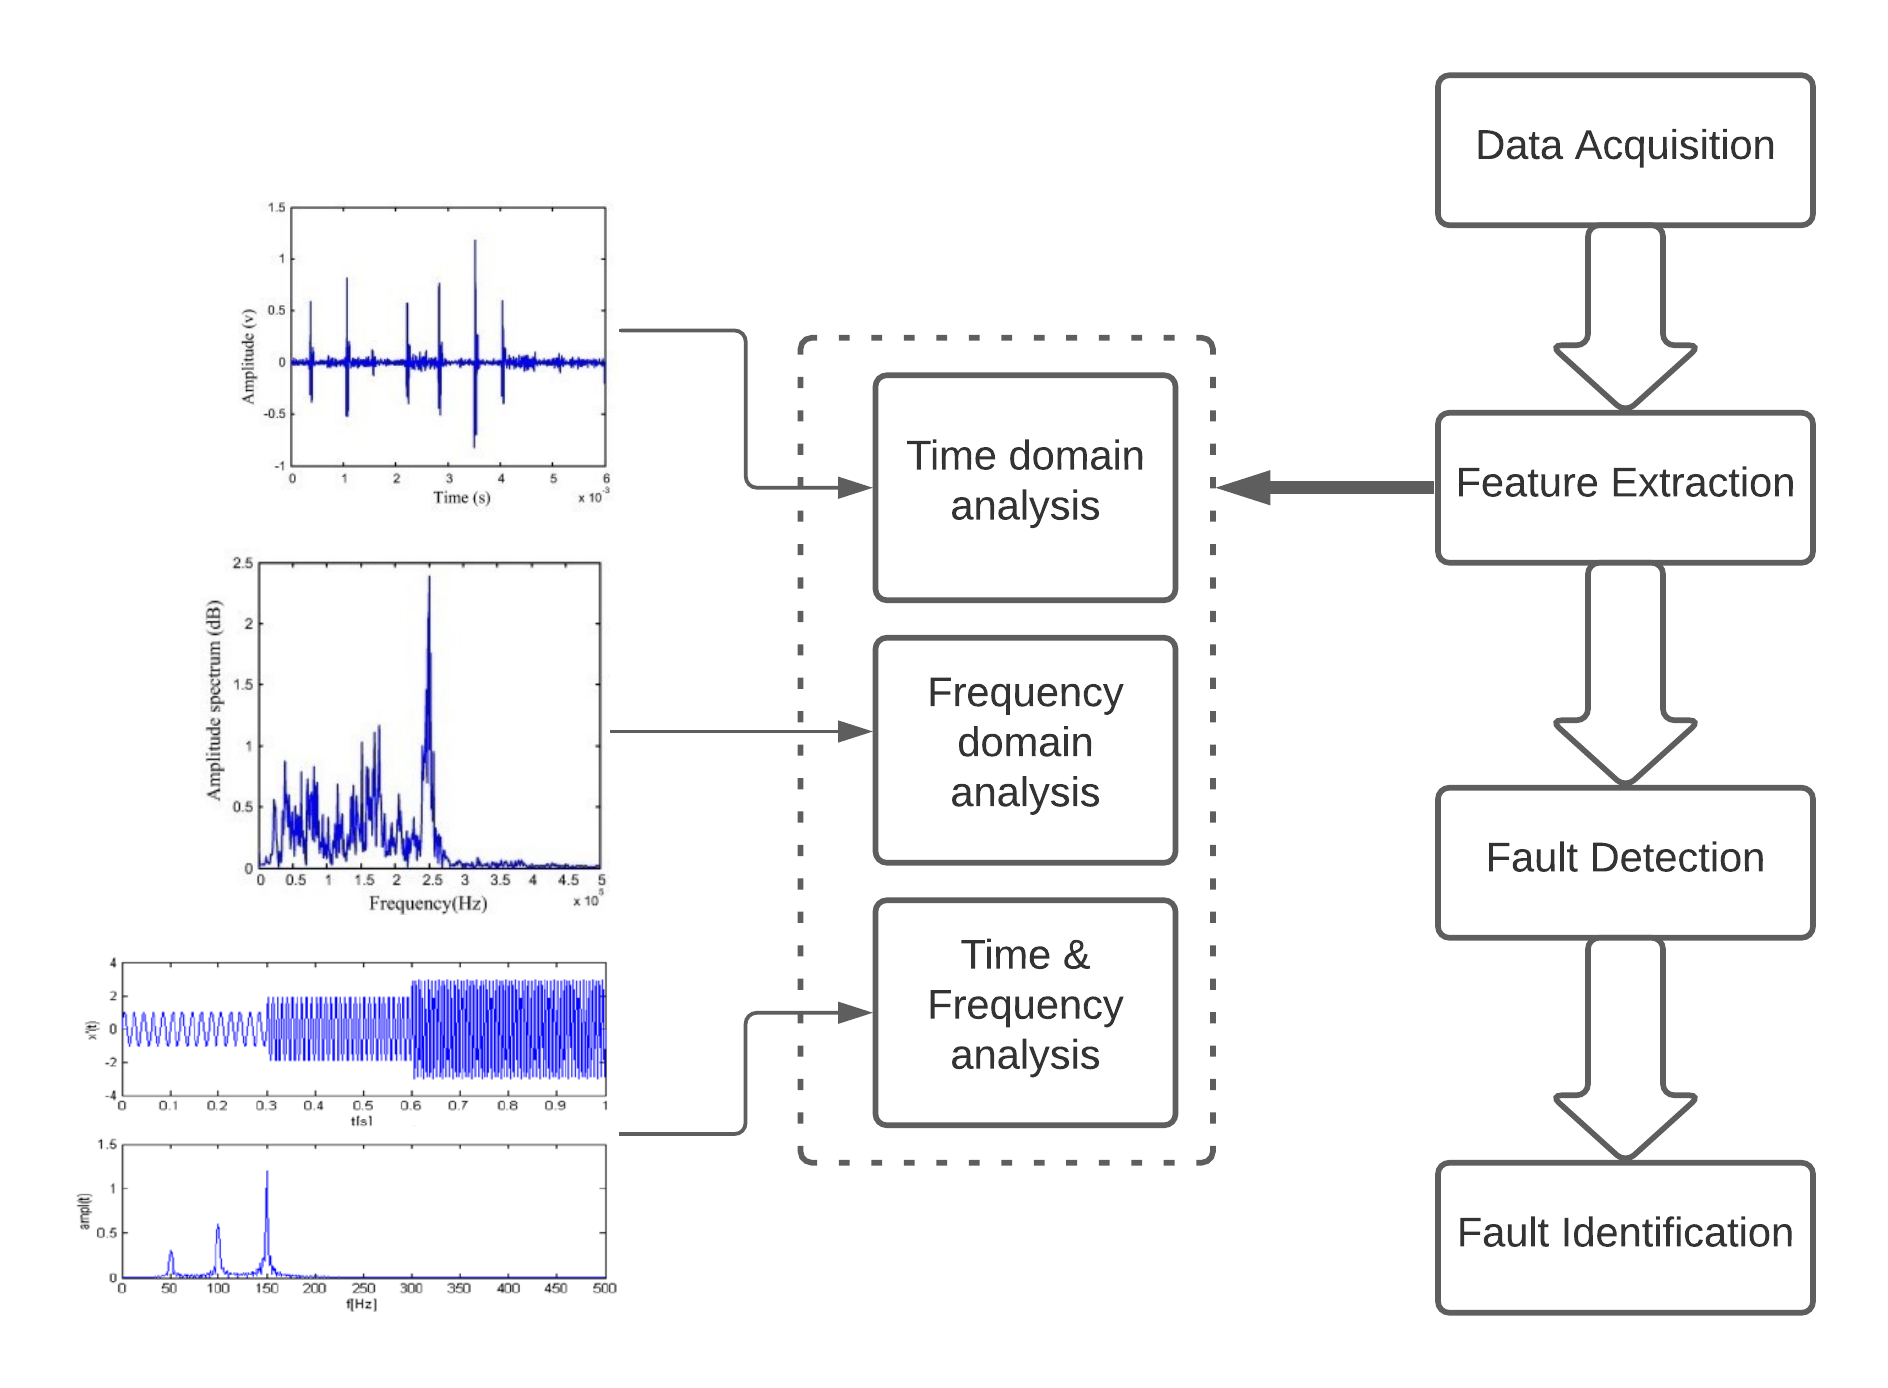
\includegraphics[width=\textwidth]{gfx/Overview of fault diagnosis based on vibration signals.png}
	\captionsetup{justification=centering}
	\caption{Overview of fault diagnosis based on vibration signals.}
	\label{fig:OverviewFaultDiagnosis}
\end{figure}
The different approaches of feature extraction are categorized into time domain, frequency domain, and time \& frequency domain methods and also include some windowing techniques that can be used in some of the methods. Whenever a method can only be used on the data of a singular sensor instead of the time series itself, we assume that the generated features we want to extract of different sensors are concatenated in one feature vector for the whole time series instance $x \in \mathcal{X}$.

\subsection{Time Domain}
\vspace*{-15mm}
\hfill{\fontfamily{phv}\normalsize\emph{Sanjay Gupta}}
\label{sec:feature-extraction:approaches:time-domain}
\\\\
The amount of vibration signals generated by the machine usually include statistical or mathematical (e.g. amplitude, acceleration, displacement, and velocity) data related to machine health.

\subsubsection*{Basic mathematical features}
Table \ref{table:BasicMathematicalFeatures} shows a list of time-domain features that are commonly used for PdM \cite{DBLP:phd/dnb/Kimotho16}. These features can be very effective in the detection of bearing failures, imbalances, mechanical loss, electrical failure of the motor, and gearbox failures. The most basic method for measuring time-domain faults is to use the value of the Root Mean Square (RMS). The RMS value and Crest factor are used to diagnose gears and bearings failures \cite{TANDON1999469}.
\begin{table}[ht]
	\centering
	\begin{tabular}{|p{3cm}|p{3cm}|p{6cm}|}
		\hline
		\vspace{-1mm} \textbf{Feature} & \vspace{-1mm} \textbf{Formula} & \vspace{-1mm} \textbf{Description} \\[3ex]
		\hline

		\vspace{-1mm} RMS Value & \vspace{-1mm} \begin{math} \sqrt{\frac{1}{n}\sum_{i=1}^{n} s_{i}^{2} } \end{math} & \vspace{-1mm} Measure the power contained in the signal. \\[3ex]
		\hline

		\vspace{-1mm} Variance & \vspace{-1mm} \begin{math} \frac{1}{n} \sum_{i=1}^{n}(s_{i}-\bar{s})^2 \end{math} & \vspace{-1mm}  Measure the variability in the signal. \\[3ex]
		\hline
		
		\vspace{-1mm} Skewness & \vspace{-1mm} \begin{math} \frac{\sum_{i=1}^{n}(s_{i}-\bar{s})^3}{(n-1)\sigma^3} \end{math} & \vspace{-1mm} Measure the asymmetry of the data around the mean. \\[3ex]
		\hline
		
		\vspace{-1mm} Entropy & \vspace{-1mm} \begin{math} - \sum_{i=1}^{n} s_{i} \log_{2}{(s_{i})} \end{math} & \vspace{-1mm} Measure the structure and complexity of time series. \\[3ex]
		\hline
		
		\vspace{-1mm} Kurtosis & \vspace{-1mm} \begin{math} \frac{1}{n} \sum_{i=1}^{n} (\frac{s_{i}-\mu}{\sigma})^4	\end{math} & \vspace{-1mm} Measure the relative peakedness or flatness of a distribution. \\[3ex]
		\hline
		
		\vspace{-1mm} Peak value & \vspace{-1mm} \begin{math} \max(|s_{i}|) \end{math} & \vspace{-1mm} Measure maximum amplitude at some time. \\[3ex]
		\hline
		
		\vspace{-1mm} Peak to peak & \vspace{-1mm} \begin{math} \max(s_{i}) - \min(s_{i}) \end{math} & \vspace{-1mm} Measure the maximum excursion of the signal. \\[3ex]
		\hline
		
		\vspace{-1mm} Crest factor & \vspace{-1mm} \begin{math} \frac{Peak}{RMS} \end{math} & \vspace{-1mm} Measure smoothness of the signal. \\[3ex]
		\hline
		
		\vspace{-1mm} Shape factor & \vspace{-1mm} \begin{math} \frac{RMS}{\frac{1}{n} \sum_{i=1}^{n}|s_{i}|} \end{math} & \vspace{-1mm} RMS divided by Mean. \\[3ex]
		\hline
		
		\vspace{-1mm} Clearance factor & \vspace{-1mm} \begin{math} \frac{Peak}{(\frac{1}{n} \sum_{i=1}^{n}|s_{i}|)^2} \end{math} & \vspace{-1mm} Peak value divided by the square of root mean. \\[3ex]
		\hline
		
		% Line integral & \begin{math} \sum_{i=1}^{n} |s_{i+1}-s_{i}| \end{math} & \\
		
		\vspace{-1mm} Impulse factor & \vspace{-1mm} \begin{math} \frac{Peak}{\frac{1}{n} \sum_{i=1}^{n}|s_{i}|} \end{math} & \vspace{-1mm} The ratio of peak values to the mean of a signal. \\[3ex]
		\hline
	\end{tabular}
	\captionsetup{justification=centering}
	\caption{Basic mathematical features.}	
	\label{table:BasicMathematicalFeatures}
\end{table}

\subsubsection*{Bag of Patterns}

The Bag of Patterns (BOP) is a time series representation that enables us to determine the structural (dis)similarities between time series data and to understand the pattern distribution of the data by examining the resulting histograms \cite{Lin2012RotationinvariantSI}. The Figure \ref{fig:OverviewBOPRepresentation} shows the representation of the BOP and the steps needed to transform the time series data into a bag of patterns. First, the BOP uses the sliding window approach to extract the subsequences from the time series and then using Piecewise Aggregate Approximation (PAA) and the Symbolic Aggregate Approximation (SAX) algorithms to transforms each subsequence into a pattern. At the end, the frequency of each pattern for each time series will be calculated. The main objective of the PAA and SAX algorithms is to reduce noise and maintain the trend of time series. The PAA algorithm consists of taking the Mean instead of back-to-back points, which reduces the number of data points. The SAX algorithm bins continuous time series data into intervals and then transforms each time series independently into a sequence of letters.

\begin{figure}[ht]
	\centering
	\includegraphics[width=\textwidth]{gfx/Overview of Bag of Patterns representation.PNG}
	\captionsetup{justification=centering}
	\caption{Overview of Bag of Patterns representation.}
	\label{fig:OverviewBOPRepresentation}
\end{figure}

\subsubsection*{Shapelet Transform}
The shapelet transform approach uses the similarity between shapelet and time 
series data as bias features for classification. Similarity measures are useful for comparing the time series data. Discriminatory similarity features are divided into three parts: similarity in time, similarity in change, and similarity in shape \cite{HILLS201305}. The advantage of using the shapelet approach is that, the shapelets are understandable and can provide useful information on the problem domain. The shapelet is defined as the time series subsequence. The shapelet transform calculates the distance between the series and the shapelet, which is the minimum of the distances between this shapelet and all the shapelets of the same length extracted from the time series data. The Figure \ref{fig:OverviewShapeletTransform} shows the transformation after applying the Shapelet Transform algorithm to the time series data and also outlines the most discriminative shapelets that have been selected.

\begin{figure}[ht]
	\centering
	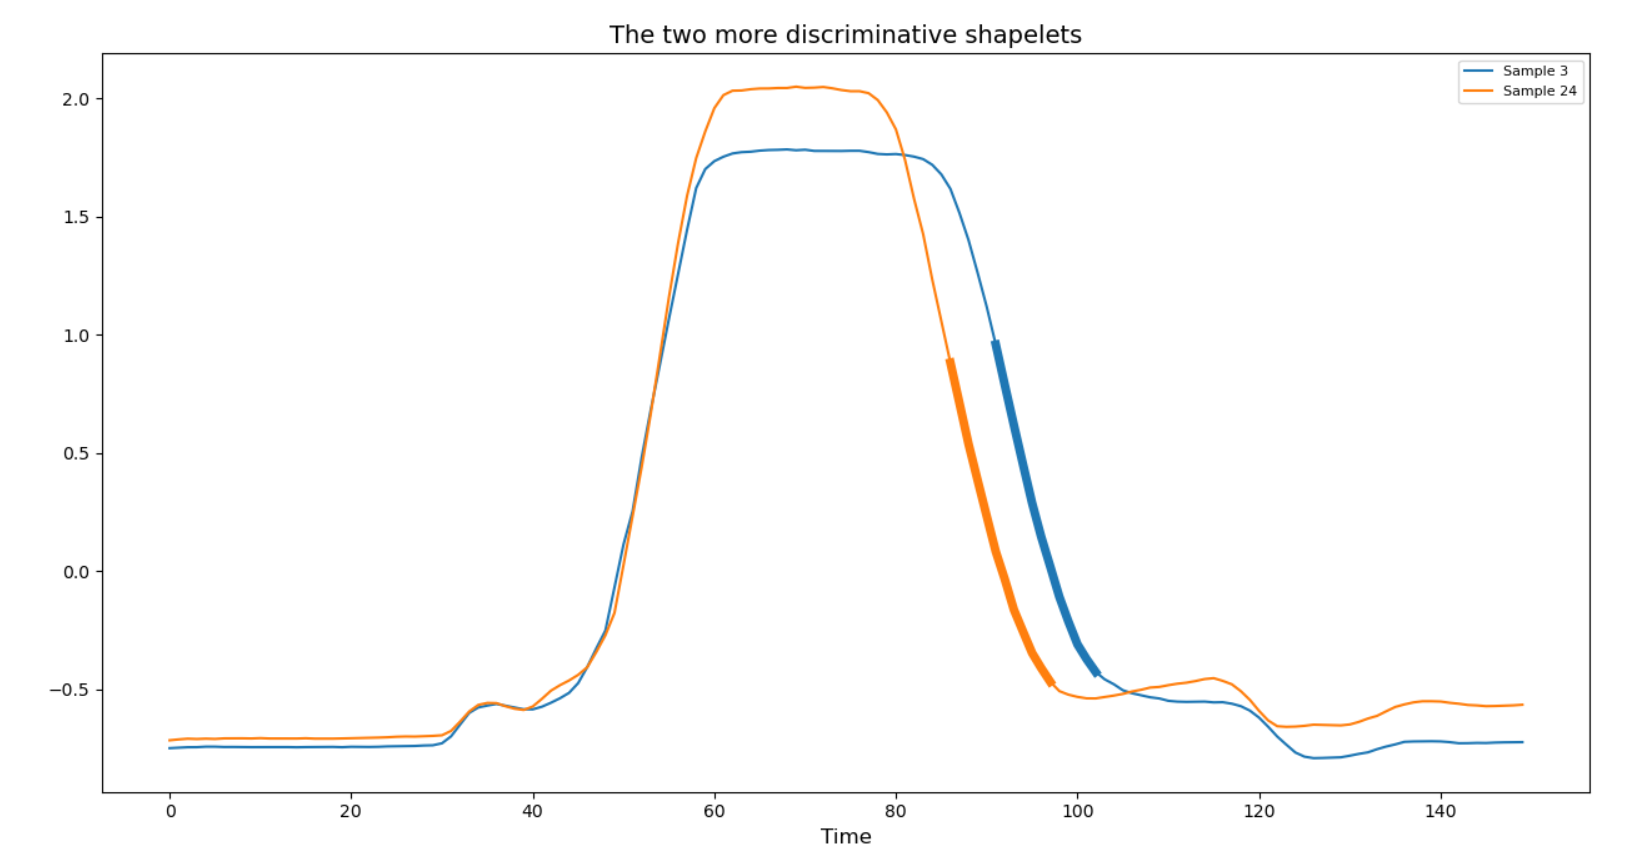
\includegraphics[width=\textwidth]{gfx/Overview of shapelet transform.png}
	\captionsetup{justification=centering}
	\caption{Example of Shapelet Transform.}
	\label{fig:OverviewShapeletTransform}
\end{figure}

\subsubsection*{ROCKET}

ROCKET stands for Random Convolutional Kernel Transform. Using random convolutional kernels, ROCKET is an exceptionally fast and accurate time series classification \cite{dempster_etal_2020}. The Figure \ref{fig:OverviewROCKET} shows an overview of the algorithm. ROCKET takes time series data as input and generates a large number of random convolutional kernels. In simple terms, the kernel is a small matrix that is used for creating a feature map from time series. In ROCKET, all characteristics (e.g. Bias, Length, Weights, Dilation, and Padding) of kernels are random. ROCKET extracts two aggregate features from each feature map produced by each convolutional kernel. The first is the maximum value, and the second is the proportion of positive values (ppv). Maximum value includes the calculation of global max pooling and global average pooling and both are used for dimensionality reduction in convolutional neural networks (CNN). In global average pooling, we take the average of each feature map, and in global maximum pooling, we take the largest value from each feature map. The ppv directly represents the proportion of the input that matches the pattern. The bias term acts as threshold for ppv: the negative bias value means strong matches between the input and the given pattern, and the positive bias value means weak matches between the input and the given pattern. The ppv is the only feature that gives higher classification accuracy. ROCKET produces 2000 (2k) features per time series for 1000 kernels (k) (e.g. max and ppv). The transformed features by ROCKET are used to train any classifier.

\begin{figure}[ht]
	\centering
	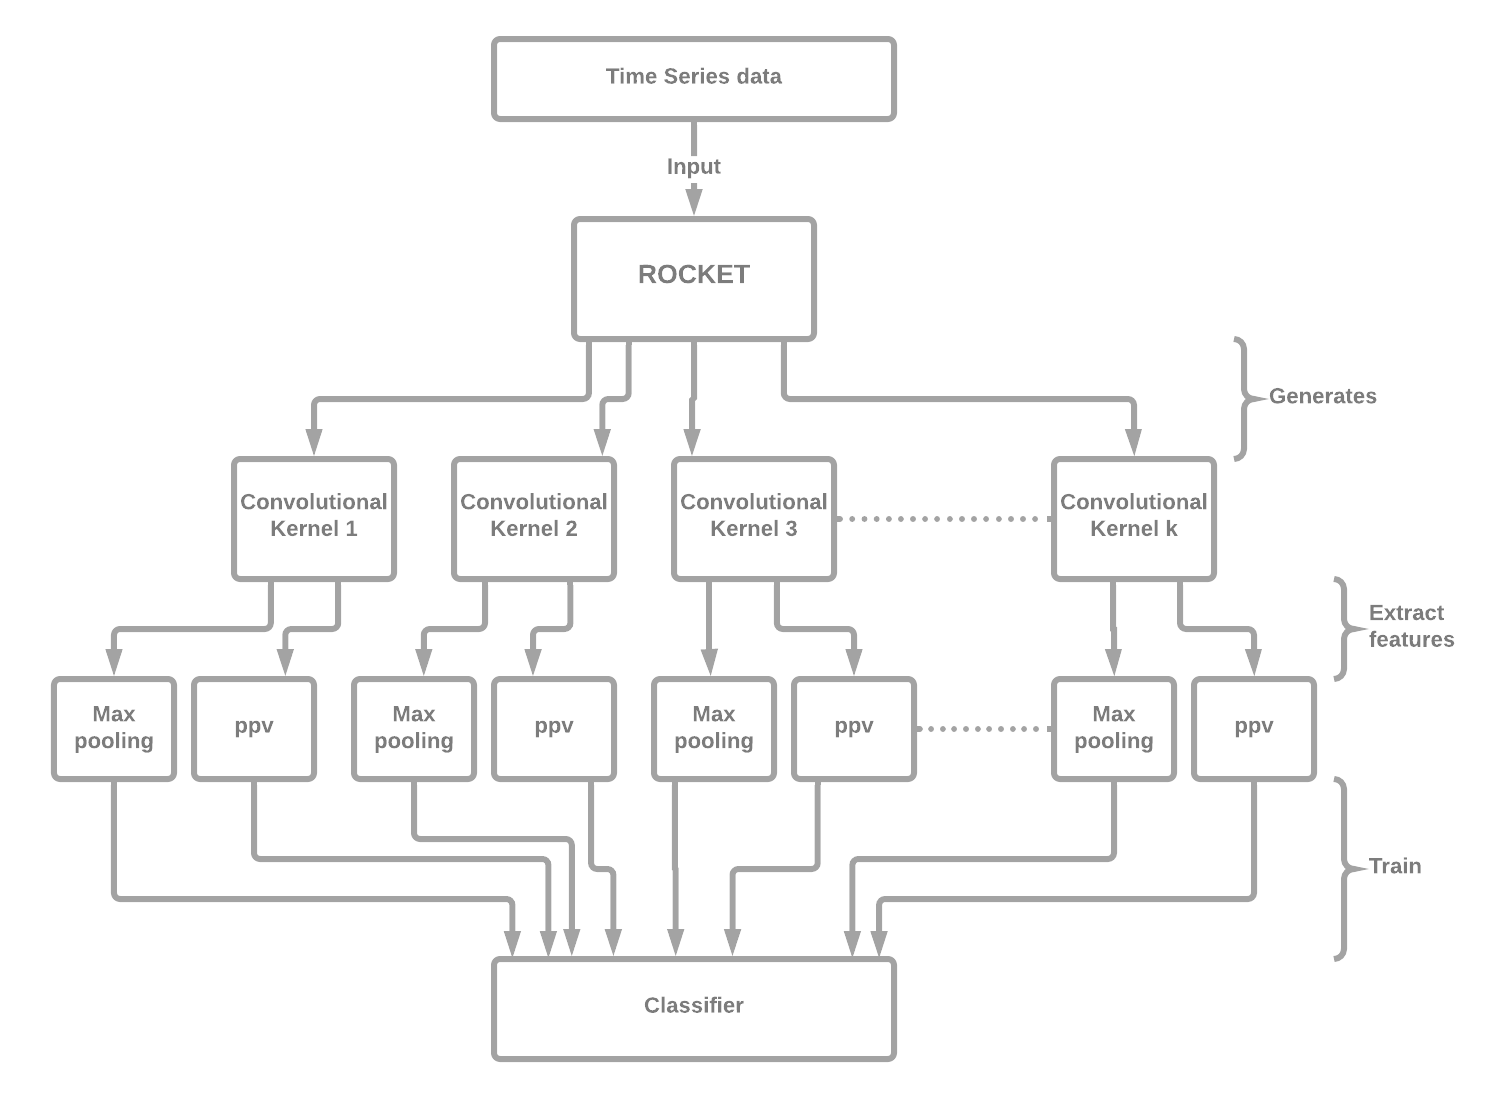
\includegraphics[width=\textwidth]{gfx/Overview of ROCKET.PNG}
	\captionsetup{justification=centering}
	\caption{Overview of ROCKET}
	\label{fig:OverviewROCKET}
\end{figure}

\subsubsection*{RNN Autoencoder}

A Recurrent Neural Network (RNN) is a powerful deep learning (DL) algorithm that works on sequential time series data. Autoencoder (AE) is an unsupervised Artificial Neural Network (ANN) that extracts features from the original data and then reconstructs the data. RNN based AE is an automatic feature extraction method that reduces noise while maintaining important information. Figure \ref{fig:StructureRNNAE} represents the structure of RNN AE consisting of an encoder and a decoder. In the RNN AE training, the input is the original time series data and the output is the reconstructed time series data. In the encoding phase, the input data is efficiently compressed and encoded  then the features are extracted. The extracted features of all frames are fed into the decoder. In the decoding phase, the data is reconstructed back from the reduced encoded representation to a representation that is as close to the original input as possible.

\begin{figure}[ht]
	\centering
	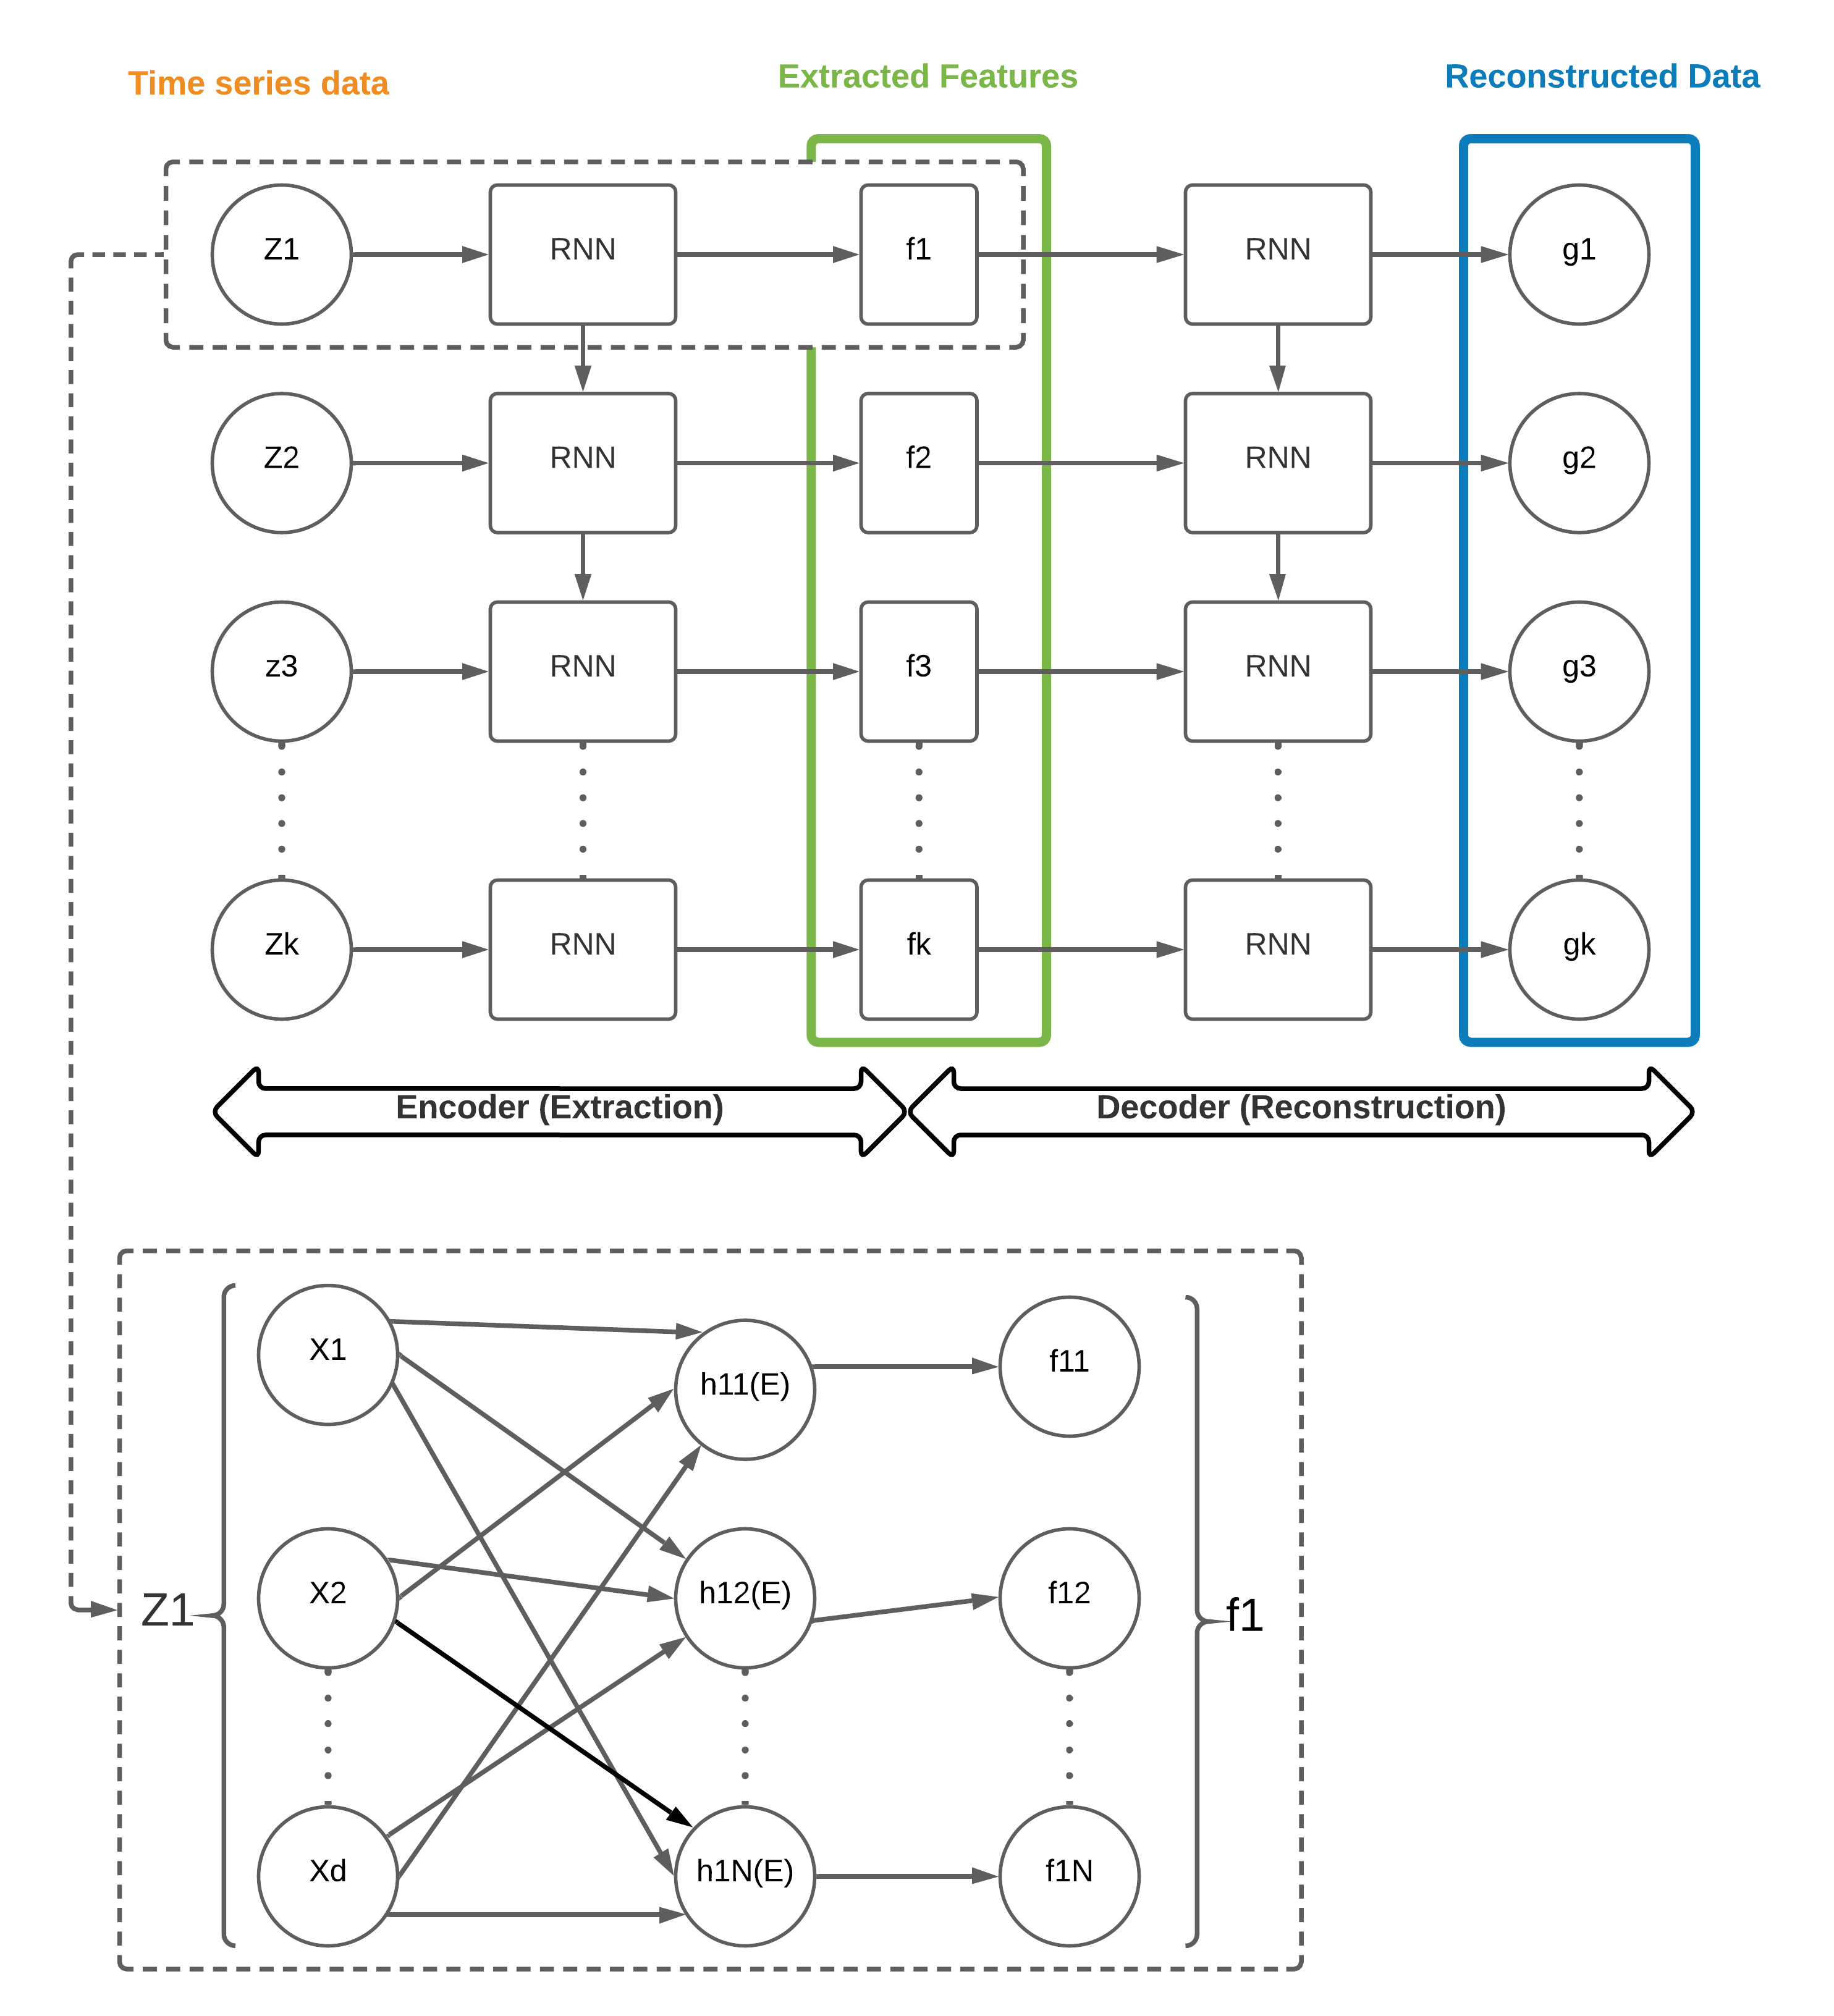
\includegraphics[width=\textwidth]{gfx/Structure of RNN AE.PNG}
	\captionsetup{justification=centering}
	\caption{Structure of the RNN AE}
	\label{fig:StructureRNNAE}
\end{figure}

\subsection{Frequency Domain}
\vspace*{-15mm}
\hfill{\fontfamily{phv}\normalsize\emph{Paul Fährmann}}
\label{sec:feature-extraction:approaches:frequency-domain}
\\\\
The frequency domain of a time series or more specifically of sensor data is a collection of frequencies that represents our sensor data. We transform our sensor data into this frequency domain via the discrete Fourier transform (DFT). We can then use different feature extraction methods to generate features which can be then combined into a real valued vector as defined in Section~\ref{sec:feature-extraction:formal-definition}.
\paragraph{Discrete Fourier Transformation}
To transform the data of sensor $s \in [S]$ of time series $x_{i}\in\mathcal{X}$ with length $l := \tau(i,s)$ into the frequency domain, we use the following function \cite{DBLP:phd/dnb/Kimotho16}:
\begin{equation}
DFT(\omega_k)=\sum\limits_{j=0}^{l-1} v_{i,s}^{(j)} e^{-u\omega_kj},\quad k = 0,\dots,l-1,
\end{equation}
where $\omega_k = \frac{2\pi k}{l}$, $v_{i,s}^{(j)} \in V(s)$ for all $j$, $u$ is the imaginary unit and $DFT(\omega_k)$ is the $k$-th coefficient. For this we can only use sensors with singular values out of a value domain  $V(s)\subseteq\mathbb{C}$.
\subsubsection{Basic Features}
Once the signal is transformed into the frequency domain with $DFT$, basic features like in the time domain can be extracted.\\
Below are a few examples \cite{DBLP:phd/dnb/Kimotho16} of features that can be extracted from the data of one sensor.
\begin{center}
	\begin{tabularx}{.625\textwidth}{ll}
		\hline
		Feature & Formula\\
		\hline
		Maximum Amplitude & $\max(DFT(\omega_k))$\\
		Frequency of Max-Amplitude & $\omega_k|_{max(DFT(\omega_k))}$\\
		Energy of signal & $\sum_{k=0}^{l-1}|DFT(\omega_k)|^2$\\
		\hline
	\end{tabularx}
\end{center}
These features can be extracted from different sensor data and then be put into a singular feature vector as a representation of the whole time series.
\subsubsection{BOSS}
Another way to utilize the frequency domain is BOSS \cite{schafer2015boss} , or Bag of Symbolic Fourier Approximation Symbols.
This method is based on the SFA algorithm and combines it with a bag-of-words approach via quantization using Multiple Coefficient Binning (MCB). Both methods are described below.
\paragraph{Symbolic Fourier Approximation (SFA)}
Transform the time series into the frequency domain using the $DFT$ as described above. Then remove most of the higher frequencies to contain the lowest $c$ coefficients. This is also called low pass filtering. Quantize the real and imaginary parts of the these $c$ Fourier coefficients and put them into words using MCB.
\paragraph{Multiple Coefficient Binning (MCB)}
This technique requires a dataset of time series which can be transformed into the frequency domain. Let's assume we have a data set of size $N \in \mathbb{N_{>0}}$.
As stated above, we take the first $c$ coefficients of each element of a dataset, that results in $N * c$ real and imaginary values. We put these in a $2c \times N$ matrix $A$, such that each row corresponds to the $c$ coefficients of one element of our dataset.
\begin{equation}
A =
\begin{bmatrix}
	\text{Re}_{11} & \text{Im}_{11} & \dots & \text{Re}_{1c} & \text{Im}_{1c} \\
	\vdots & \vdots & \ddots & \vdots & \vdots \\
	\text{Re}_{N1} & \text{Im}_{N1} & \dots & \text{Re}_{Nc} & \text{Im}_{Nc} \\
\end{bmatrix}
\end{equation}
with Re and Im as the real and imaginary values.
We sort the column by value and use equi-depth binning with a prior defined alphabet $\sum$ of size $m\in\mathbb{N_+}$ to create $m$ intervals, which separate the $m$ letters of that alphabet.
\begin{figure}[ht]
	\centering
	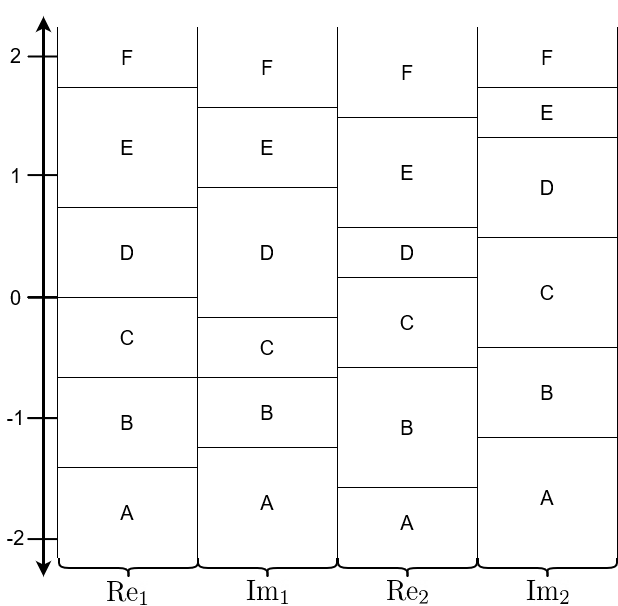
\includegraphics[width=.8\textwidth]{gfx/BOSS_MCB2.PNG}
	\caption{Breakpoints for MCB - example with $m = 6$ and $c = 2$}
	\label{fig:BOSS_MCB}
\end{figure}
In Figure~\ref{fig:BOSS_MCB} we see an example of the MCB with $2$ coefficients, resulting in $2$ real and $2$ imaginary values and an alphabet size of $6$. Transforming a time series into its word using this example we do the following:
\begin{enumerate}
	\item Transform the time series into the frequency domain using $DFT$.
	\item Retain only the first $2$ coefficients, resulting in $4$ values, $2$ real and $2$ imaginary values.
	\item Look in the intervals defined in Figure~\ref{fig:BOSS_MCB} to transform each value into the corresponding letter of the alphabet of size $6$.
	\item Concatenate these letters to one word, representing the time series.
\end{enumerate}
By concatenating the letters to a word we form the word representing the time series. This can be then put into a feature vector for a representation.\\
One question still remains on how to transform the word into the feature representation, defined in Subsection~\ref{sec:feature-extraction:formal-definition}, as this requires a real-valued representation vector.
There are several approaches on how to represent the word in this vector form. We map the letters of the alphabet using $f : \sum \rightarrow \mathbb{R}$ to certain fixed values. Given the intervals for the letters we can take the average value of the interval as a representation of that letter. The mapping $f$ is a bijection; thus we can regain the original word by using the same mapping in reverse.
\subsection{Time and Frequency Domain}
\vspace*{-15mm}
\hfill{\fontfamily{phv}\normalsize\emph{Paul Fährmann}}
\label{sec:feature-extraction:approaches:time-frequency-domain}
\\\\
Using both the time domain and frequency domain of the sensor data of a time series we can extract new types of features that cannot be extracted using just the time or just the frequency domain. We explain two of those approaches.
\subsubsection{Discrete Wavelet Transform (DWT)}
The general motivation for wavelet transforms is, that the frequency domain alone does not provide information on the time in which the frequencies are localized. The wavelet transform tries to solve that by "scanning" over the time series using wavelets of different lengths. When we define the wavelet transform in an abstract way, we arrive at the continuous wavelet transform. We are however interested in the actual application and hence the discrete wavelet transform \cite{DBLP:journals/iet-spr/SangeethaH17}. That is a decomposition of a time series into an amplitude function over two dimensions: time and frequency. This is done using wavelets, which are oscillations with start and end at amplitude value 0. They are used as a sliding filter that is put over the data signal. We need to be able to translate and stretch this filter. In the end, we are able to calculate wavelet coefficients that can be used for a feature vector of the given time series.\\
We need to define when a function or time series $\psi(j)$ is a \textit{wavelet}. $\psi(j)$ is a \textit{wavelet} if the Fourier transformation of $\psi(j)$, named $DFT(\omega_\psi)$ satisfies the following condition:
\begin{equation}
	C_\psi := \int_{0}^{\infty}\frac{|DFT(\omega_\psi)|^2}{|\omega_\psi|} d \omega_\psi < \infty
\end{equation}
This condition describes that the energy of this wave is finite, such that the amplitude will trail off to zero on both sides. 
\begin{figure}[ht]
	\centering
	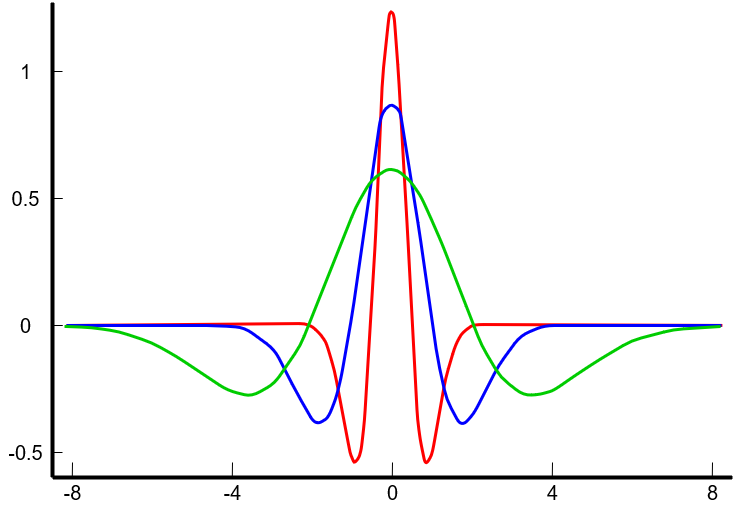
\includegraphics[width=0.5\textwidth]{gfx/DWT_wavelet2.PNG}
	\caption{three examples of wavelet functions.}
	\label{fig:DWT_wavelet}
\end{figure}
Once we have such a wavelet like in Figure \ref{fig:DWT_wavelet}, we can define the discrete wavelet transform as follows:
\begin{equation}
	D[a,b] = \frac{1}{\sqrt{b}}\sum_{j=0}^{l-1} v_{i,s}^{(j)} \psi \left[ \frac{t_{i,s}^{(j)} - a}{b}\right]
\end{equation}
with $l := \tau(i,s)$, $a = k2^{-p}$ and $b = 2^{-p}$.
The parameters $a$ and $b$ stretch and translate the wavelet. Using different values for $a$ and $b$ we scan over the time and over the frequency domain of the original signal. Defining these parameters in the given form where we choose the parameters $k$ and $p$, we assure a dyadic wavelet transformation which has useful properties \cite{DBLP:journals/iet-spr/SangeethaH17}.
Scanning over the original data with different dyadic wavelets we can generate wavelet coefficients which are amplitudes located in time and frequency. These can be viewed as functions that can be analyzed using above mentioned basic time and frequency domain approaches.
\subsubsection{Empirical Mode Decomposition (EMD)}
In the empirical mode decomposition \cite{huang1998empirical} we want to decompose the original time series into intrinsic mode functions (IMF). There is not a lot of mathematical theory behind this method but it transforms the data into a more useful form. 
The idea here is to define a band in which the original data lies. For that an upper \textit{envelope} and a lower \textit{envelope} are defined, such that every value of the original series lies between those envelopes.
For a function to be an IMF, it has to fulfill the two IMF conditions: 
\begin{enumerate}
	\item When counting the  local extrema and the number of crossings through 0, the resulting counts of both must differ by at most 1.
	\item The mean value of the upper and lower envelopes must be equal to zero at every point in the sensor data.
\end{enumerate}

\begin{figure}[ht]
	\centering
	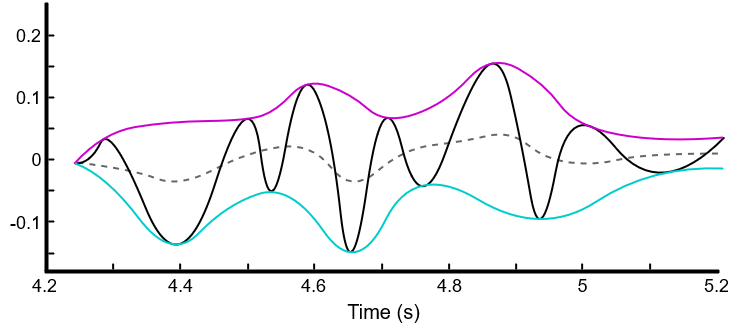
\includegraphics[width=\textwidth]{gfx/EMD_envelopes2.PNG}
	\caption{Example of a time series (black) with upper (magenta) and lower (cyan) envelopes as well as the mean (gray, dashed) of these envelopes.}
	\label{fig:EMD_envelopes}
\end{figure}
These \textit{envelopes} are defined by local minima (lower \textit{envelope}) and local maxima (upper \textit{envelope}) of the original sensor data. To connect these local extrema to a function we use cubic-spline interpolation as seen in Figure~\ref{fig:EMD_envelopes}. Each extrema is connected to the next extrema via a polynomial function of degree 3 \cite{DBLP:journals/computing/Gfrerer82}.  
Once we have generated the envelopes, we can calculate the mean of these \textit{envelopes}. To calculate the IMF components, we need to use the following sifting process.
\paragraph{Sifting process for $v_{i,s} = h_{10}$}:\\
We subtract the mean of the envelopes from the original data to create a new series of values.
\begin{equation}
	 v_{i,s} - m_{10} =: h_{11}
\end{equation}
where $m_{10}$ is the mean of the envelopes on the original data signal and $h_{11}$ is the new series of values for the first step of sifting.
If the conditions for an IMF are not fulfilled, repeat the this sifting step with the new series $h_{11}$ in the place of $v_{j,s}$ to generate $h_{12}$. That means calculating the upper and lower \textit{envelopes} of $h_{11}$ and subtracting the mean $m_{11}$ of these \textit{envelopes} from our series $h_{11}$ creating $h_{12}$.
\begin{equation}
	h_{11} - m_{11} =: h_{12}
\end{equation}
This sifting process step is repeated until $h_{1m_1}$ fulfills the IMF conditions.
\paragraph{IMF components}
The first IMF component can then be defined as $c_1 = h_{1m_1}$.
Repeating this sifting process with $h_{20} := v_{i,s} - c_1$, we generate $c_2$.
Following this procedure, we can calculate $c_1, \dots , c_n$ as the $n$ IMF components.\\
To generate our feature vector we can use the basic features of the time and the frequency domain on these IMF components and put these into one vector representation of the time series $v_{i,s}$.

\subsection{Windowing techniques}
\vspace*{-15mm}
\hfill{\fontfamily{phv}\normalsize\emph{Sanjay Gupta}}\label{sec:feature-extraction:approaches:windowing}
\\\\
In windowing techniques, time series data is partitioned into several windows with specific lengths, from which vector features are 
extracted and fed to a machine learning classifier. One of the widely used windowing techniques is the sliding window technique.

\subsubsection*{Sliding Windows}
The sliding window method is the most widely used approach in the time series classification. In this approach, the time series 
data is divided into fixed-size windows. If there is an intersection between the two adjacent windows, then this technique is 
called an overlapping sliding window and, if not, it is known as a non-overlapping sliding window. The Figure \ref
{fig:SlidingWindows} shows overlapping and non-overlapping techniques for sliding windows. Each window is transformed into a vector 
of features that are mostly time domain, frequency domain, or time \& frequency domain features. This set of features is then used 
to train different classifiers. The number of data points in the window has a significant impact on the performance of the 
model. However, in any case, the size of the window should be selected in such a way that each window contains enough samples to be 
distinguishable from similar movements. Most of the time, window length is selected by trial and error method. The number of sliding 
windows to be used differs for each algorithm of time series classification. While BOSS used a single sliding window to extract 
words, Word Extraction for time Series cLassification (WEASEL) used many sliding windows of different sizes to extract words \cite
{DBLP:conf/cikm/SchaferL17}. The BOP algorithm uses a sliding window to extract subsequences from time series data. Due to a large 
amount of time series data, the performance of the overlapping sliding window increases compared to the non-overlapping sliding 
window.
\begin{figure}[ht]
	\centering
	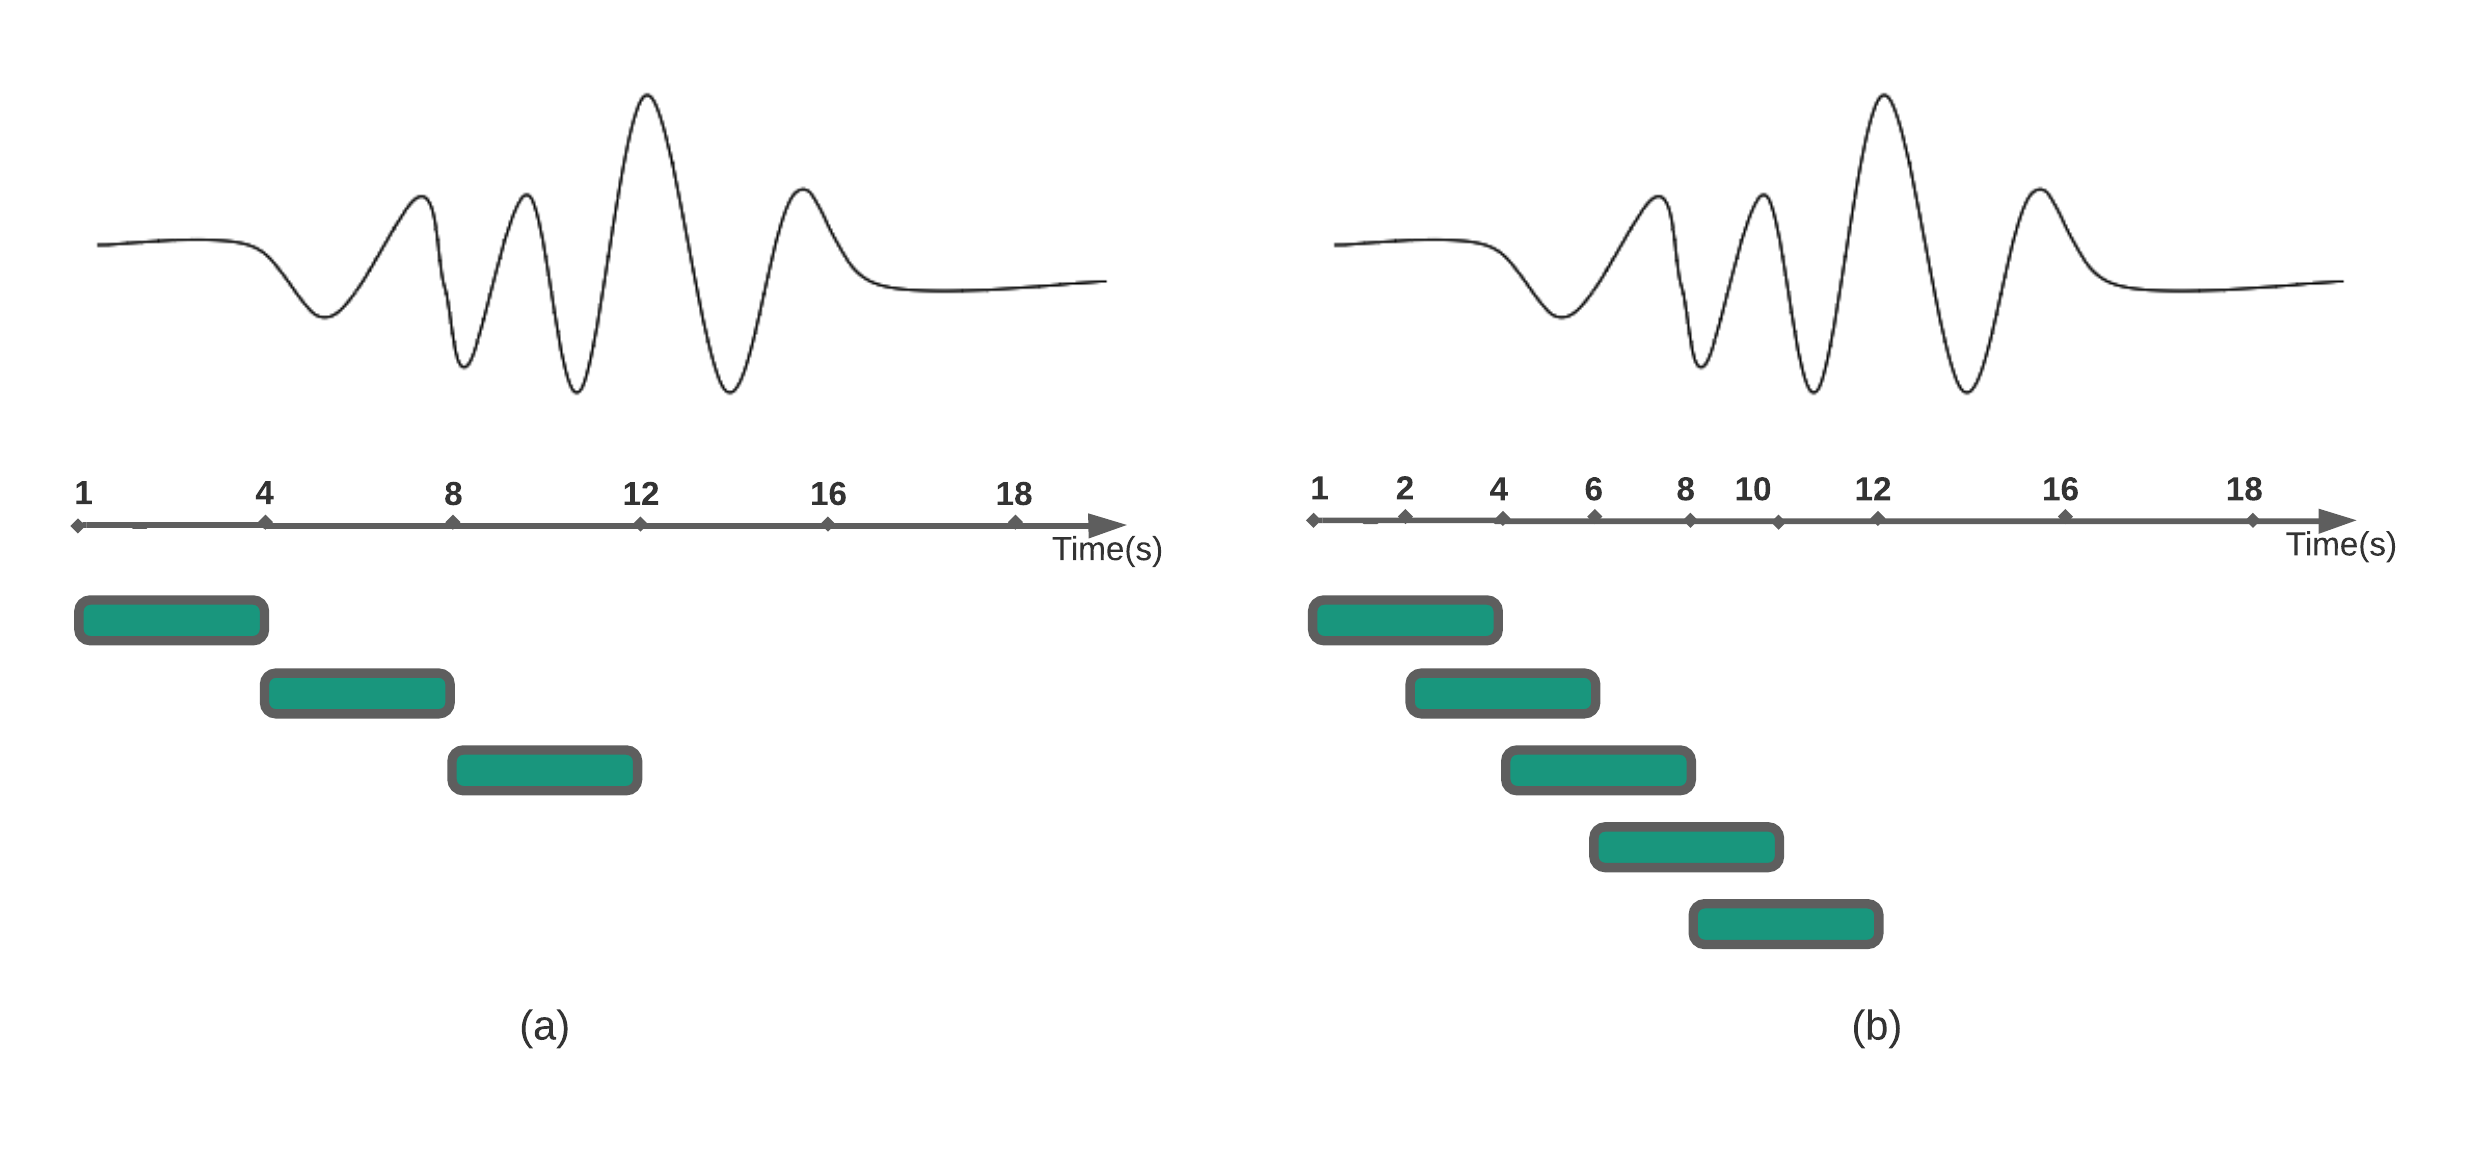
\includegraphics[width=\textwidth]{gfx/Sliding windows.png}
	\captionsetup{justification=centering}
	\caption{4s sliding windows. (a) Non-overlapping; (b) Overlapping-2s sharing.}
	\label{fig:SlidingWindows}
\end{figure}
% Approaches Setion end.

% Evaluation Setup start.
\section{Evaluation Setup}
\vspace*{-15mm}
\hfill{\fontfamily{phv}\normalsize\emph{Paul Fährmann}}
\label{sec:feature-extraction:evaluation-setup}
\\\\
For the evaluation of a feature extraction method, we can look at the feature set or feature vector that this method creates. In order to evaluate a feature vector, we look how well it can be used in various classification or regression problems.\\
In general, we can use the classification and regression models from the following chapters and the loss functions that are used there for our evaluation setup.
In detail that means we control for the entire pipeline except the feature vector and the loss of the model. The loss of the model can then be interpreted as a loss for the feature vector. By swapping different feature vectors in the same setup, the loss for these different feature vectors can be determined. These losses can be compared to each other and so determined what the better and what the worse feature vectors are. It also shows which feature extraction method, on average, performs better on a dataset.
It is important to note though, that the evaluation of a feature extraction method is only meaningful in the specific context or pipeline in which the evaluation was done.
But it can be used for feature selection. The method that extracts the most useful features will get the best evaluation on their extracted feature vectors for this exact pipeline setup. We can then fix the pipeline further by fixing the feature extraction method.\\
A concrete, simple example for this evaluation setup would be a classification problem using the feature vectors of time series of a labeled dataset and the leave-one-out cross validation 
with the $k$-nearest neighbor ($k$-NN) classifier. The evaluation setup would now look as follows:
\begin{enumerate}
	\item Fix the pipeline: fixed model, choose $k$ (e.g. $k = 5$) and the distance metric (e.g. euclidean distance)  for $k$-NN as well as the loss function (e.g. RMSE = root mean square error). Also fix the dataset $\mathcal{X}$.
	\item Transform all $x \in \mathcal{X}$ into their feature vectors via $g_1(x) = z \in \mathbb{R}^d$ with a feature extraction method $g_1$.
	\item Use leave-one-out cross validation with the loss function and the $k$-NN model to calculate the average loss over the entire dataset $\mathcal{X}$.
	\item Repeating step 2 and 3 with $g_2, \dots, g_m$ for $m$ different feature extraction methods. We can compare the average loss for these feature extraction methods and thus evaluate them.
\end{enumerate}
This example demonstrates the evaluation setup for a simple classification scheme. The same setup can be adapted to various different classification and regression schemes. For that we replace parts of this setup. For example, for a regression problem we would replace the model with a regression model and use a loss function for regression problems. Again the leave-one-out cross validation loss over a data set is then used as an evaluation for the used feature vector.
\paragraph{Leave-One-Out Cross Validation}
Given a loss function $l$, a model $M$ and a data set $\mathcal{X}$. The leave-one-out cross validation is given by generating $R := |\mathcal{X}|$ training sets $\mathcal{X}/\{x_i\}$ with $x_i \in \mathcal{X}$ for $i \in [R]$. We train the model $M$ on these data sets, generating fully trained models $M_1, \dots, M_R$. Then we evaluate the classification/regression for the one left out instance, e.g. for $M_1$ we calculate the loss with $l$ for the instance $x_1 \in \mathcal{X}$.
Averaging the loss over all the trained models and evaluated instances, we get the leave-one-out cross validation.

% Evaluation Setup end.

% \section{Related Work Section 2}
% \label{sec:related:sec2}

% \Blindtext[3][2]

% \section{Related Work Section 3}
% \label{sec:related:sec3}

% \Blindtext[4][2]

% \section{Conclusion}
% \label{sec:related:conclusion}

% \Blindtext[2][1]
                    % INCLUDE: feature extraction
% !TEX root = ../main.tex
%
\chapter{Health State Classification}
\label{sec:system}

\cleanchapterquote{A healthy outside starts from the inside.}{Robert Urich}{(Actor)}\newline 
\vspace*{-15mm}
\hfill{\fontfamily{phv}\normalsize\emph{Anurose Prakash}}\newline 
\newline 

In the entire life cycle of industrial machinery, the machines undergo a series of health degradation states from time to time till it reaches to a complete failure state. The historical knowledge of the health transition associated with the existing machinery can be used to predict the upcoming changes that the same machinery will undergo. This is utilized by the health state probability estimation techniques to monitor the entire cycle of failure degradation using supervised classification algorithms. These algorithms produce health state probabilities as an output that is better suited for the prognostic approach of PdM since the health state probabilities can be combined with the historical lifetimes of similar systems at each health state to estimate the RUL. The fault diagnosis techniques such as fault classification differ from health state classification in a way that the former focuses on the occurrences of the faults within the system, whereas the latter tries to provide inputs to RUL prediction methods.\newline 

\section{Motivation}
\vspace*{-15mm}
\hfill{\fontfamily{phv}\normalsize\emph{Saghar Heidari}}
\label{sec:system:sec1}

The PdM in general and health state estimation particularly aims to assess the current state of a system or machine to avoid high costs associated with system failure and reactive maintenance and to keep system or machines operable for longer periods of time. Thanks to developments in controlling technologies (e.g. sensors) and IT (high-performance  computers etc.), the implementation of such systems received growing attention. In particular, Health state classification plays a vital role in designing a condition monitoring system by providing useful information about the current state of a machine or a system. Knowing the health state of a system or a machine, we are able to estimate the asset's remaining useful life e.g. the time after that some parts of the system should be replaced to prevent a break down in the system. It shows also the deviation of the health state of a system or a machine from its healthy state which causes a quality reduction in the output of the system or may cause the system or machine failure in the future. Therefore, the health state estimation enables us to take appropriate action to keep a system or a machine healthy and to avoid possible failures in the future.

Regardless of which classification model is used, several steps are needed to take us from raw time series data to a classifier that can get future time series data and predict the health status of the machine or system as shown in Figure \ref {fig:Pipeline}.
To achieve that, we split data into two sub-groups of train and test. The training dataset is used to train the model or classifier and the test data will be used to validate the model and show how good a model or classifier is in predicting the class labels.

\begin{figure}[H]
    \centering
    \includegraphics[width=8cm]{gfx/Pipeline.png}
    \captionsetup{justification=centering}
    \caption{Pipeline of health state classification}
    \label{fig:Pipeline}
\end{figure}

\section{Formal problem definition}
\vspace*{-15mm}
\hfill{\fontfamily{phv}\normalsize\emph{Anurose Prakash}}
\label{sec:system:sec2}

The data-driven supervised health state classification techniques works on time series data $x_i$(cf. \ref{sec:intro:time-series-definition}). The input data to the training process $D_{train}$ contains $x_i$ and and corresponding health state label $l_i$ $\in$ $L$ where $L$ is a set of possible health states(i.e. healthy, faulty, failure) at each time step $i$ $\in$ $[T(i,s)]_1^{\tau(i,s)}$ of input time series. Training data consists of $N \in \mathbb{N}$  samples at an instance $i$ of historic data and is of the form:
\begin{equation}
  D_{train} = \{(x_i,l_i)\}_{i=1}^N  
\end{equation}


The test data $D_{test}$ involving $M \in \mathbb{N}$ samples consists of $x_i$ that denotes the recorded time series data and the actual health state label $y_i$ $\in$ $L$. 
\begin{equation}
  D_{test} = \{(x_i,y_i)\}_{i=1}^M  
\end{equation}

The trained classification model $h$ is subjected to test data $D_{test}$ without true health state label $l_i$ to get the predicted health state label $\hat{y_i}$ where $\hat{y_i}$ = $h(x_i)$ for each instance $i$ of recorded data. Then, the performance of prediction is estimated with the help of loss function $\mathcal{L}$ defined as:
$\mathcal{L}$($D_{test}$) = $\Sigma_{i=1}^N$ [\, $\hat{y_i}$ = $y_i$ ]\,
which uses true label $y_i$ from the test dataset against predicted label $\hat{y_i}$. Further details on the loss functions that evaluate the classification approaches involved in this chapter will be explained in section \ref{sec:system:sec5}.


\section{Available Datasets}
\vspace*{-15mm}
\hfill{\fontfamily{phv}\normalsize\emph{Saghar Heidari}}
\label{sec:HS:datasets}

In this section, two datasets, namely Condition monitoring of hydraulic systems dataset and Bearing Fault Dataset are introduced. The former collects the data from a hydraulic test rig and the latter contains the data of a bearing test rig.
\subsection{Condition monitoring of hydraulic systems dataset}
\vspace*{-5mm}
\hfill{\fontfamily{phv}\normalsize\emph{Saghar Heidari}}

The condition monitoring of hydraulic systems dataset \cite{CMOHS} contains 17 tab-delimited text files (*.txt) which stored time series data of 17 sensors (14 Physical and 3 virtual)  from a hydraulic test rig. This test rig includes a primary working and a secondary cooling-filtration circuit which are connected via the oil tank. The system was designed to repeat constant load cycles of 60 seconds and to measure process values, namely pressures, volume flows, and temperatures, and to store variations in the condition of hydraulic components of the system cooler, valve, pump, and accumulator. Table \ref{tab:Description_table1} shows the attribute information from the measurement of sensor data at the same point in time.


\begin{table}[ht]
 \centering
\begin{tabular}{|c|c|c|l|}
\hline
Sensor & Physical Quantity          & Unit    & Sampling Rate \\ \hline
PS1-6  & Pressure                   & Bar     & 100Hz         \\ \hline
FS1-2  & Volume Flow                & l/min   & 10Hz          \\ \hline
TS1-4  & Temperature                & Celsius & 1Hz           \\ \hline
EPS1   & Motor Power                & W       & 100Hz         \\ \hline
VS1    & Vibration                  & mm/s    & 1Hz           \\ \hline
CE     & Cooling Efficiency (Virt.) & \%      & 1Hz           \\ \hline
CP     & Cooling Power (Virt.)      & KW      & 1Hz           \\ \hline
SE     & Efficiency Factor          & \%      & 1Hz           \\ \hline
\end{tabular}
\vspace{0.3cm}
\captionsetup{justification=centering}
\caption{Sensor data description and their attribute information }
\label{tab:Description_table1}
\end{table}

 The target values which represent the condition of hydraulic components of the system are stored in another tab-delimited text file (profile.txt) in which the target condition values are cycle-wise annotated (see Table \ref{tab:Description_table2}).
The dataset has been used in feature extraction tasks (e.g.\cite {DBLP:conf/i2mtc/HelwigPS15}) as well as supervised classification tasks monitoring of degradation in health states (e.g.\cite{helwig2015d8}).


\begin{table}[ht]
\centering
\begin{tabular}{|c|c|c|l|}
\hline
\begin{tabular}[c]{@{}c@{}}Column Nr.\\  (in profile.txt)\end{tabular} & Component Name        & Unit & Conditions                                                                                                                            \\ \hline
1                    & Cooler                & \%   & \begin{tabular}[c]{@{}l@{}}3 Close to Failure\\ 20 Reduced Efficiency\\ 100 Full Efficiency\end{tabular}                                                 \\ \hline
2                    & Valve                 & \%   & \begin{tabular}[c]{@{}l@{}}100 Optimal\\ 90 Small Lag\\ 80 Severe Lag\\ 73 Close to total Failure\end{tabular}                                           \\ \hline
3                    & Internal Pump Leakage & -    & \begin{tabular}[c]{@{}l@{}}0 No Leakage\\ 1 Weak Leakage\\ 2 Severe Leakage\end{tabular}                                                                 \\ \hline
4                    & Hydraulic Accumulator & Bar  & \begin{tabular}[c]{@{}l@{}}130 Optimal Pressure\\ 115 Slightly Reduced Pressure\\ 100 Severely Reduced Pressure\\ 90 Close to total Failure\end{tabular} \\ \hline
5                    & Stable Flag           & -    & \begin{tabular}[c]{@{}l@{}}0 Conditions were Stable\\ 1 Static Conditions might\\    not have been reached yet\end{tabular}                              \\ \hline
\end{tabular}
\vspace{0.3cm}
\captionsetup{justification=centering}
\caption{Description of hydraulic components of the system with their conditions}
\label{tab:Description_table2}
\end{table}\newpage

\subsection{Bearing Fault Dataset}
\vspace*{-15mm}
\hfill{\fontfamily{phv}\normalsize\emph{Saghar Heidari}}

The bearing fault dataset \cite{dataset} includes nominal bearing data, an inner race fault, and an outer race fault at various loads from a bearing test rig which is shown in Table \ref {sec:datasets:Bearing_table}. It also contains three real-world faults, namely intermediate speed bearing, oil pump bearing, and planet bearing. 
\begin{table}[ht]
\centering
\begin{tabularx}{\textwidth}{| X | X | X | X | X | X|}
\hline
\textbf{Nr. of files in Dataset} & \textbf{State}			& \textbf{Load (lbs)}   & \textbf{Input Shaft Rate (Hz)} & \textbf{Sampling Rate (sps)} & \textbf{Duration (s)}\\ \hline
3			    & Baseline (Healthy) 		& 270  & 25  & 97656	& 6 			\\ \hline
3			& Outer Race Fault		& 270  & 25	  & 97656	& 6 \\ \hline
7		& (Further) Outer Race Fault		& 25,50,100, 150,200, 250,300	 & 25  & 48828	& 3		\\ \hline
7		& Inner Race Fault		& 0,50,100, 150,200, 250,300	& 25	& 48828	  & 3	\\ \hline
\end{tabularx}
\vspace{0.3cm}
\captionsetup{justification=centering}
\caption{Bearing fault Datasets description}
\label{sec:datasets:Bearing_table}
\end{table}

The data is stored in a Matlab double-precision, binary format *.mat file. Each file consists of the load, shaft rate, sample rate, and a vector of signals (gs) which can be used to differentiate between healthy and faulty states (namely outer race fault, inner race fault). This dataset has been used in feature extraction tasks as well as condition monitoring tasks \cite{bechhoefer2016quick}.

\section{Feature selection}

\vspace*{-15mm}\hfill{\fontfamily{phv}\normalsize\emph{Anurose Prakash and Saghar Heidari}}

After finding a set of features from the given data through different feature extraction methods, a subset of features that affect the target variables is selected. The main goal of feature selection is to remove redundant data and reduce dimensionality.
There are three kinds of feature selection methods, namely filter methods, wrapper methods, and embedded methods. One of the wrapper methods is the Boruta algorithm \cite{hasan2020health} which employs the random forest classification algorithm.

\subsection{Boruta algorithm}
First, it duplicates a set of features to generate shadow features. Then, it trains shadow features with a classifier, such as a Random Forest Classifier. Now, the importance of feature attributes for original and shadow features is calculated by using the Z score. If the original features have a higher Z score than the maximum importance of all shadow features, then it is recorded in a vector (Hits). The algorithm is repeated until all variables are classified. Finally, the best original features are selected from the Hit vector. 
After selecting the best features, the state-of-the-art approaches for estimating health states are considered.

\subsection{Distance Evaluation Method}

It is one of the most prevalent feature selection techniques that takes into consideration the features that help to separate each of the health state classes associated with the classification process to a maximum extent. For a set of features defined as $j = 1,2,...,Q$ associated with $c = 1,2,...N_c$ health states, the technique proceeds as below \cite{DBLP:phd/dnb/Kimotho16}:
\begin{enumerate}
    \item Features are normalized between 1 and 0.
    \item The mean of each normalized feature $x_j$ in class $c$ is calculated as:
    \begin{equation}
        m_{jc} = \frac{1}{n} \sum_{i=1}^n x_{ijc}
    \end{equation}
    \item The mean of the squared Euclidean distance between each feature data point $i$ and mean of its associated  feature is computed as:
    \begin{equation}
        d_j = \frac{1}{N_c^2 n}\sum_{k=1}^{N_c} \sum_{c=1}^{N_c} \sum_{i=1}^n (x_{ijk} - m_{jc})^2
    \end{equation}
    \item The evaluation criteria of the feature selection process is derived by normalizing the separation distance with maximum possible feature separation distance.
    \begin{equation}
        \bar d_j = \frac{d_j}{max(\bar d)}
    \end{equation}
    \item A distance is selected that is greater than the predetermined threshold whose value depends on the classification accuracy for given set of features.
\end{enumerate}

\section{Health state estimation using supervised learning techniques}
%\vspace*{-15mm}
\hfill{\fontfamily{phv}\normalsize\emph{Anurose Prakash and Saghar Heidari}}
\label{sec:system:sec4}

The classification models identify the current health state using features extracted from condition monitoring data. The optimal selection of the features determines the performance of the machine learning algorithm and this is ensured with the help of the feature selection techniques mentioned above. The following subsections discuss the background of various classification models used as part of health state estimation.\newline


\subsection{Support vector machines (SVM)}
\vspace*{-12mm}\hfill{\fontfamily{phv}\normalsize\emph{Anurose Prakash}}

Support Vector Machines (SVM) is considered as one of the most efficient classification algorithms with its excellent generalization ability in comparison to traditional machine learning methods such as neural networks \cite{Kim2010MachinePB}. The paper highlights the abilities of SVM in terms of maximum margin classifier that simultaneously minimizes the empirical classification error and maximizes the geometric margin. It has the potential to handle very large feature spaces because the training of SVM uses the dimension of classified vectors without degrading classification performance. As per author, SVM was originally created for binary classification purposes where it seeks to find a hyperplane that separates data into two classes within the feature space, with the largest margin possible. 
\begin{figure}[ht]
	\centering
	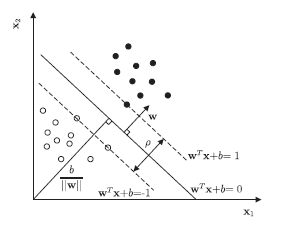
\includegraphics[scale=1.0]{gfx/SVM_1.PNG}
    \captionsetup{justification=centering}
	\caption{SVM hyperplane for binary classification of linearly separable data}
	\label{fig:SVM structure}
\end{figure}
Figure 1 \cite{DBLP:journals/tist/ChangL11} shows the basic principle of SVM for classification. Figure \ref{fig:SVM structure} depicts the bounding planes that are parallel to the hyperplane bordering each of the sub-classes and the data points that lie on the bounding planes called as support vectors \cite{DBLP:journals/tist/ChangL11}. For a given set of $n$ training samples ${x_i, y_i}$ such that $i \in n$ and each of the sample has $Q$ features ($x_i \in R^Q$) and class label with one of the binary values ($y_i \in \{-1, 1\}$), a hyperplane is a $n-1$ dimensional plane as:
\begin{equation}
    w^T x + b = 0
\end{equation}
where $w$ denotes a vector orthogonal to the hyperplane and $b$ is a constant\cite{DBLP:phd/dnb/Kimotho16}. Such a hyperplane
$(w, b)$ that separates data defines the function:
\begin{equation}
    f(x) = sgn(w^T x + b)
\end{equation}
In classifying problems, a larger margin $\rho$ means a better classification accuracy separating the two data classes and it involves minimizing $w$. A detailed derivation of binary classification of linearly separable data is described in paper by Kimotho\cite{DBLP:phd/dnb/Kimotho16}.

In the case of non-linearly separable data, SVM employs a kernel function as mentioned in table \ref{sec:SVM:Kernal} to transform the input data into a higher dimensional feature space where classification is carried out \cite{Burbidge2001AnIT}. 
\begin{table}[h]
    \centering
	\begin{tabularx}{\textwidth}{| X | X |}
		\hline
		\textbf{Kernal functions} & \textbf{$K(x_i,x_j)$}\\\hline
		Linear & $x_i^T x_j$\\ \hline
		Polynomial of power $p$ & $(1 + x_i^T x_j)^p$\\\hline
        Radial basis function & $exp(-\gamma || x_i - x_j ||^2)$\\\hline
        Multi-layer perceptron & $tanh(\gamma_0 x_i^T x_j + \gamma_1)$\\\hline
    \end{tabularx}
    \captionsetup{justification=centering}
	\caption{Kernal functions in SVM}
    \label{sec:SVM:Kernal}
\end{table}
\vspace*{-4mm}
The health state classification deals with the classification of more than one health states found during the degradation stages of machine lifetime, hence the multiple instances of binary SVM classifier is combined to achieve multi-classification. Strategies such as "One-Against-One(OAO)", "One-Against-All(OAA)" and "Directed Acyclic Graph SVMs" are used to perform the health state probability estimation of discrete failure degradation stages. A comparison of these strategies was done and OAO is found as leading over the other two in practical terms\cite{DBLP:journals/tnn/HsuL02}. In OAO, for given observations $x_t = (x_{t_1}, x_{t_2},...,x_{t_m})$, where $m$ is the number of observations in hand and $t$ is the timestep. Assuming $y_t$ as the health state at time $t$ and $y_t$ = 1,2,...,$n$, where n is the number of health states. For the multi-classification of $n$-health state events, the one-against-one method has $n(n-1)/2$ classifiers, where each classifier is trained on data from two classes. For training data from the $i^{th}$ and the $j^{th}$ classes, SVM solves the following classification problem:
\begin{equation}
\begin{split}
    minimize : 1/2 {|| w^{ij}||}^2 + C\sum_{t} \xi_j^{ij}(w^{ij})^T\\
    subject\:to: (w^{ij})^T \psi(x^t) + b^{ij}\geq 1 - \xi_j^{ij}, \; if y_t = i,\\
    (w^{ij})^T \psi(x^t) + b^{ij}\leq -1 + \xi_j^{ij}, \; if y_t = j,\\
    \xi_j^{ij} \geq 0 , \; j = 1, 2, ..., l
    \end{split}
\end{equation}

Here, the training data is mapped to a higher dimensional vector by function $\psi$ and $\psi(x^t)$ is considered as kernel function, $(x_t,y_t)$ is the $i^{th}$ or $j^{th}$ training sample, $w \in R^n$ is the coefficient vector, $b \in R$ is the bias
of the hyper-plane, $\xi_t^{ij}$ is the slack variable and $C$ is the penalty parameter. After a series of
tests, the decision is made using the following strategy: if sign $(w^{ij})^T \psi(x^t) + b^{ij}$ denotes $x_i$ to be in $i^{th}$ class then the class is added by one; otherwise, the $j^{th}$ value is increased by one.\newline
From the above SVM multi-classification result $(y_t)$, the probabilities of each health states $(S_t)$ is derived using the smooth window and indicator function $(I_i)$ as following: 
\begin{equation}
    \begin{split}
        Prob(S_t = i|\overrightarrow{x_t}, ..., \overrightarrow{x}_{t+u-1}) = \sum _{j=t}^{t+u-1} I_i(y_j)/u\\
        I_i = \left\{
        \begin{array}{ll}
          0, & \mbox{if $y \neq i$}.\\
          1, & \mbox{otherwise}.
        \end{array}
      \right.
    \end{split}
\end{equation}

As the probability of one state decreases, the probability of the next state increases. At the point of intersection there is a region of overlap between the two health states, which is a natural phenomenon in linear degradation process as depicted in Figure \ref{fig:SVM structure2}. However, the probability distribution of failure process is complex due to the dynamic and stochastic degradation process in a real world scenarios.
\begin{figure}[ht]
	\centering
	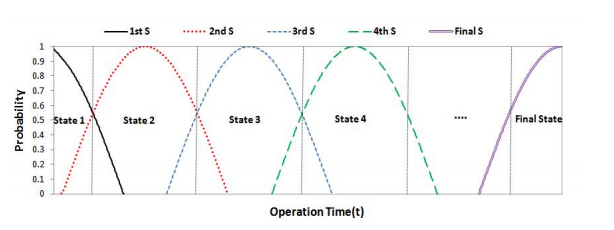
\includegraphics[scale=0.9]{gfx/svm_2.PNG}
    \captionsetup{justification=centering}
	\caption{Health state probability distribution for linear degradation process. \cite{Kim2010MachinePB}}
	\label{fig:SVM structure2}
\end{figure}

\subsection{Deep Belief Networks(DBN)}
\vspace*{-12mm}\hfill{\fontfamily{phv}\normalsize\emph{Anurose Prakash}}

Deep Belief Networks(DBN) classifier is one of the popular deep machine learning approaches that consists of a hierarchical structure with multiple layers of Restricted Boltzmann Machines (RBM). This approach utilises the advantages of deep learning such as fast inference and the ability to encode richer and higher order network structures \cite{DBLP:journals/ress/TamilselvanW13}. The author describes a DBN based health state estimation technique that has three consecutive stages:
\begin{enumerate}
    \item Collecting sensory data for DBN training and testing.\vspace*{-3mm}
    \item Developing DBN based classification models for the diagnosis of predefined health states.\vspace*{-3mm}
    \item Validating DBN classification models with testing sensory dataset\vspace*{-3mm}
\end{enumerate}
The structure of DBN is a layered architecture made up of multiple layers of RBMs with one visible layer and more than one hidden layer. 
\begin{figure}[ht]
	\centering
	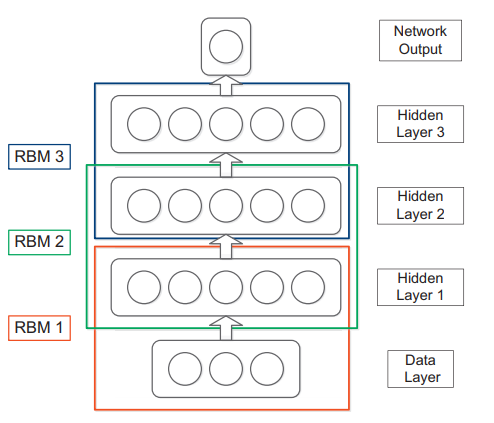
\includegraphics[scale=0.8]{gfx/dbn1.png}
    \captionsetup{justification=centering}
	\caption{DBN Structure.\cite{DBLP:journals/ress/TamilselvanW13}}
	\label{fig:DBN structure}
\end{figure}

\begin{figure}[ht]
	\centering
	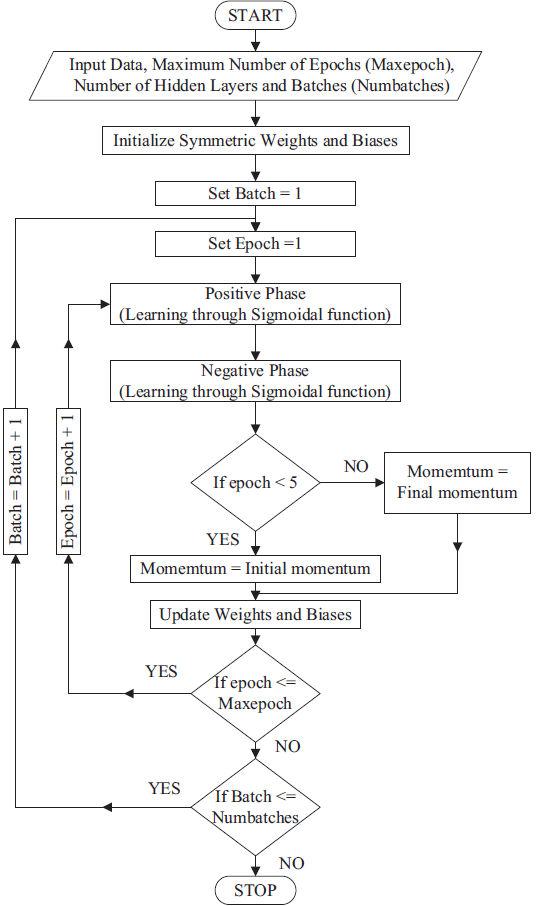
\includegraphics[scale=0.6]{gfx/dbn3.png}
    \captionsetup{justification=centering}
	\caption{Each iteration of RBM unit learning \cite{DBLP:journals/ress/TamilselvanW13}.}
	\label{fig:DBN_layer_structure}
\end{figure}
The visible layer of a DBN accepts the input data and transfers the data to the hidden layers. Figure \ref{fig:DBN structure} shows a DBN structure with 3 layers of RBMs. Layer 1 and layer 2 denotes the first RBM and similarly for the other layers. Each of the connected RBM layers undergoes the same transformation concept leading to a regular learning process within the structure. The training process of DBN involves two stages, i.e. training the RBM unit by means of the RBM learning rule and performing the back propagation supervised learning. The RBM learning rule consists of two steps - the positive and the negative phases as depicted in Figure \ref{fig:DBN_layer_structure}.
The positive learning phase transfers data from the bottom visible layer to the hidden layer and derives the probability of generating hidden units as $p(h|v,W)$. Its is formally defined as :
\begin{equation}
P(h_j = 1|v) = sigm ( -b_j - \sum_k v_k w_{jk} )    
\end{equation}

The negative phase operates as a reconstruction of the data from previous visible layer and determines the probability of generating visible units as $p(v|h,W)$ formally stated as:
\begin{equation}
P(v_k = 1|h) = sigm ( -b_k - \sum_j v_j w_{jk} )    
\end{equation}
\vspace*{-1mm}
Here, $w_{jk}$ denotes the synaptic weight updated as part of learning process in the respective positive and negative phases represented as:
\begin{equation}
    \Delta w_{jk} = \delta(\langle v_k h_j \rangle_{data} - \langle v_k h_j \rangle_{recon}) 
\end{equation}
where $\delta$ is learning rate and has values between 0 and 1, $\langle v_k h_j \rangle_{data}$ is pairwise product of the state vectors for the $j^{th}$ neuron in the hidden layer and the $k^{th}$ neuron in the visible layer after the positive phase learning process,whereas $\langle v_k h_j \rangle_{recon}$
denotes the pairwise product after the negative phase learning process for reconstruction of the visible layer. The overall system function of DBN learning procedure is defined as the probability of generating a visible vector ($v$) denoted as $p(v)$ which is function of weights and hidden vectors based on RBM learning rule as:
\begin{equation}
    p(v) = \sum_h p(h|v,W) p(v|h,W)
\end{equation}

The transformation function in the training process is sigmoid transformation that modifies the data from one layer to another and it is represented as:
\begin{equation}
    P(s_i = 1) = \frac{1}{1 + exp(-b_i - \sum_j s_j w_{ij})}
\end{equation}
where, $s_i$ and $b_i$ corresponds to the state and bias of $i^{th}$ neuron in the hidden layer, $s_j$ is the state of $j^{th}$ neuron in the visible layer and  $w_{ij}$ stands for synaptic weight between $i^{th}$ and $j^{th}$ neuron. Momentum $m$ is used for stabilizing the RBM learning process and it updates the synaptic weights and biases. The weight update of the current epoch gets updated with previous epoch as:
\begin{equation}
    \Delta w_{jk} = (m[\Delta w_{jk}]_{n-1}) + \delta(\langle v_k h_j \rangle_{data} - \langle v_k h_j \rangle_{recon})
\end{equation}
\begin{figure}[t]
	\centering
	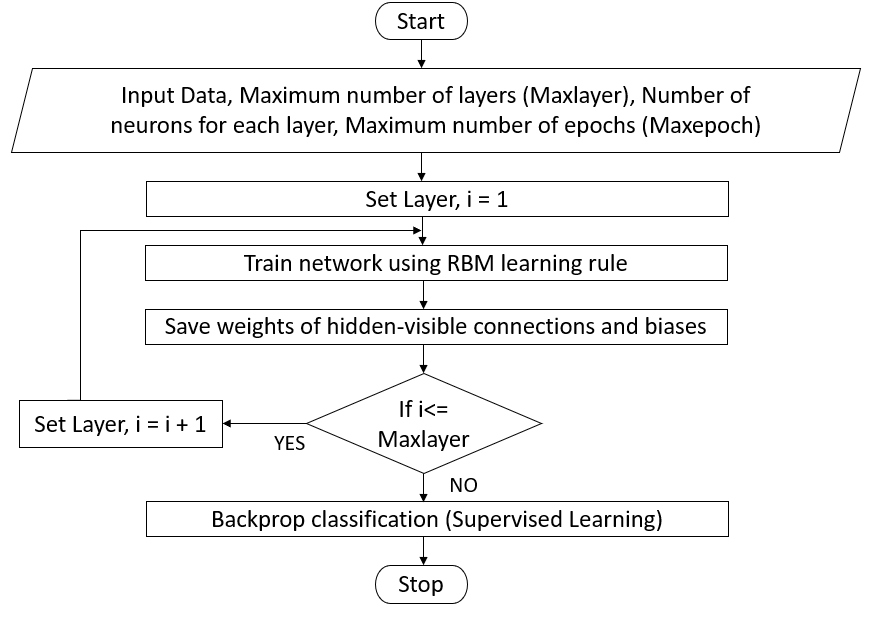
\includegraphics[scale=0.4]{gfx/Ed_dbn2.PNG}
    \captionsetup{justification=centering}
	\caption{DBN training process \cite{DBLP:journals/ress/TamilselvanW13}.}
	\label{fig:DBN_training_structure}
\end{figure}
As illustrated in Figure \ref{fig:DBN_training_structure}, the input to training model consisting of pre-processed batch data, the total number of layers in the DBN classifier model, the total number of hidden neurons in each hidden layer, and number of epochs are initialized. Within each layer of the training process, each of the involved RBM is individually trained and the weights and biases are saved for further analysis. Weights between visible and hidden layers and biases of the neurons in each DBN layer are optimized until the maximum number of epochs reached. The layer by layer training is followed by a supervised back-propagation training mechanism that considers all DBN layers simultaneously. The back-propagation learning is continued until the network output reaches the maximum number of epochs. This involves training the multi-layer neural network of the back-propagation network by computing error derivatives obtained after hidden layer activities and updating the weights as per requirement. Following this, the trained DBN classifier model can be further fine-tuned to improve the classification accuracy through certain fine-tuning algorithms. The weight file is used to determine the classification error.

\subsection{Logistic Regression (LR)}
\vspace*{-12mm}\hfill{\fontfamily{phv}\normalsize\emph{Anurose Prakash}}

Logistic Regression(LR) is a well-known classification model in ML with the lowest algorithm complexity. As this technique belongs to supervised learning, the collected data must have corresponding health state labels to be fed into the model. LR models have a close resemblance to the machine degradation process with its logic S-curve \cite{CAESARENDRA20101161}. This model is implemented with manifold regularization (LRMR), where it is further proposed for tool health assessment and online prediction\cite{DBLP:journals/asc/Yu18}. It is capable of estimating the failure time point of the tool with high accuracy and calculation efficiency. The logistic probability function for a logit model $g(x)$ is:
\begin{equation}
    P(x) = \frac{1}{1 + e^{-g(x)}}
\label{eq:lr}
\end{equation}
Given the n training samples, ${(x_i, y_i),
i = 1, ..., n}$, where each $x_i \in R^m$ is an m-dimensional feature vector,and $y_i \in \{0, 1\}$ is a class label, LR is defined as follows:
\begin{equation}
    log \frac{\pi_i}{1-\pi_i} = \beta_0 + \sum_{j=1}^m \beta_j x_{ij} \Leftrightarrow \pi_i = \frac{1}{1 + e^{-(\beta^T x_i)}}
\end{equation}
where $\pi_i$ denotes $p(y_i = 1|x_i,\beta)$, and $\beta$ = $(\beta_0, \beta_1, ...\beta_m)$ denotes the
vector of regression coefficients including a constant or intercept $\beta_0$. The prediction probability $P(x)$ of an event occurrence by LR is constrained between 0 and 1, which is considered as a health indication (HI) for quantifying the tool health state, i.e.,
\begin{equation}
HI_t = P(x_t)    
\end{equation}

where $P(x_t)$ can be calculated by using Eq. \ref{eq:lr}. The LRMR algorithm is used to construct LR to achieve the predicted LPs (i.e., $HI_t$). In order to improve the sensitivity and reliability of the HI (i.e., LP) to the slight degradation of tool health, the exponentially weighted moving average (EWMA) statistic of the LPs is used as an improved HI of tool health.

\subsection{Neuro-Fuzzy}
\vspace*{-15mm}
\hfill{\fontfamily{phv}\normalsize\emph{Saghar Heidari}}

The condition of a system or machine is in most cases not completely good or bad but something in between. Therefore, fuzzy logic helps to deliver this kind of uncertain knowledge in a way that is understandable for computers. Indeed, these kinds of approaches automatize the processes which should be done by a human in the past but still keeps the process interpretable and understandable using linguistic variables \cite{zeraoulia2005simple}.
The neural networks are good at reasoning tasks based on parallel computation and high speed and keep working in case of missing some piece of information while they are not able to explain how some certain decisions are attained. The fuzzy systems instead can explain system behaviors through rules and their performance can be modified by changing rules. As knowledge acquisition is in most cases not an easy task, the use of fuzzy systems is limited to the fields about which expert knowledge is available and the input data also is small.
The hybrid solutions like Neuro-Fuzzy Systems (NFS) combine both systems to get a more practical system. NFS is part of the soft computing concept.  
Neural networks can recognize patterns using a sufficient number of examples without prior knowledge. In contrary to neural networks, for fuzzy systems the prior knowledge, explicit linguistic rules, is needed if there is a lack of information or missing information the system should be tuned. In fact, neuro-fuzzy systems are neural networks that optimize certain parameters of fuzzy systems (e.g. membership function) or preprocess the data and extract fuzzy rules from data.\\
There are several types of NFS. The Mamdani-type and the Takagi-Sugeno-type \cite{Rutkowski2009} (also known as Adaptive Neuro-Fuzzy Inference System or ANFIS) neuro-fuzzy systems are the most famous types.

\subsubsection*{Fuzzy Systems:}
Every fuzzy system \cite{Rutkowski2009} consists of four components as follows (see Figure \ref{fig:Fuzzy Inference System}):\\\\
\textit{1: A fuzzifier}: It converts the input data into a fuzzy set.\\
\textit{2: A rule base}: It has fuzzy IF-THEN Rules which are provided by experts for making a decision.\\
\textit{3: A fuzzy inference engine}: It employs fuzzy reasoning techniques to determine the matching degree of input with respect to fuzzy IF-THEN rules.\\
\textit{4: A defuzzifier}: It converts the fuzzified output into crisp output.

\begin{figure}[H]
    \centering
    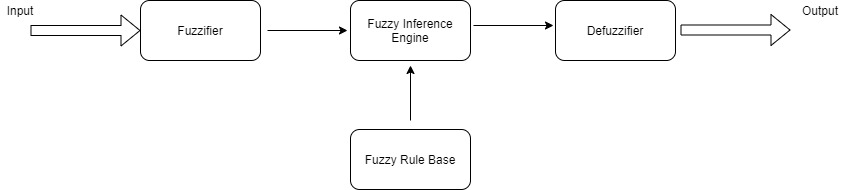
\includegraphics[width=14cm]{gfx/Fuzzy_Inference_System.png}
    %\vspace{0.3cm}
    \captionsetup{justification=centering}
    \caption{Fuzzy Inference System}
    \label{fig:Fuzzy Inference System}
\end{figure}

\subsubsection*{Formal Definitions:}
Given $x$ and $y$, as two linguistic variables (e.g. High Temperature and imminent Failure) are  $A$ and $B$, ${A}'$and ${B}'$ are fuzzified input and output accordingly the ${B}'$ can be resulted by fuzzified input ${A}'$ and relationship $R$, where relationship $R$ is \cite{Rutkowski2009}:
\begin{equation}
 IF\;\;\,  x\;\; is\,\, A\;\;\,  THEN\;\;  y\;\; is\,\, B   
\end{equation}

We face the challenge of estimating the membership function of the fuzzy relation denoted by:
\begin{equation}
    \mu _{{B}'}\left ( y \right )= \mu _{A\rightarrow B}\left ( x,y \right )
\end{equation}
Based on the knowledge of $\mu_{A}\left ( x \right )$ and  $\mu_{B}\left ( y \right )$ we can rewrite the membership function as follows:
\begin{equation}
    \mu _{A\rightarrow B}\left ( x,y \right )=I\left(\mu_{A}\left ( x \right ),\mu_{B}\left ( y \right ) \right)
\end{equation}

Figure \ref{fig:Different forms of membership functions} shows various type of membership functions.
\begin{figure}[H]
    \centering
    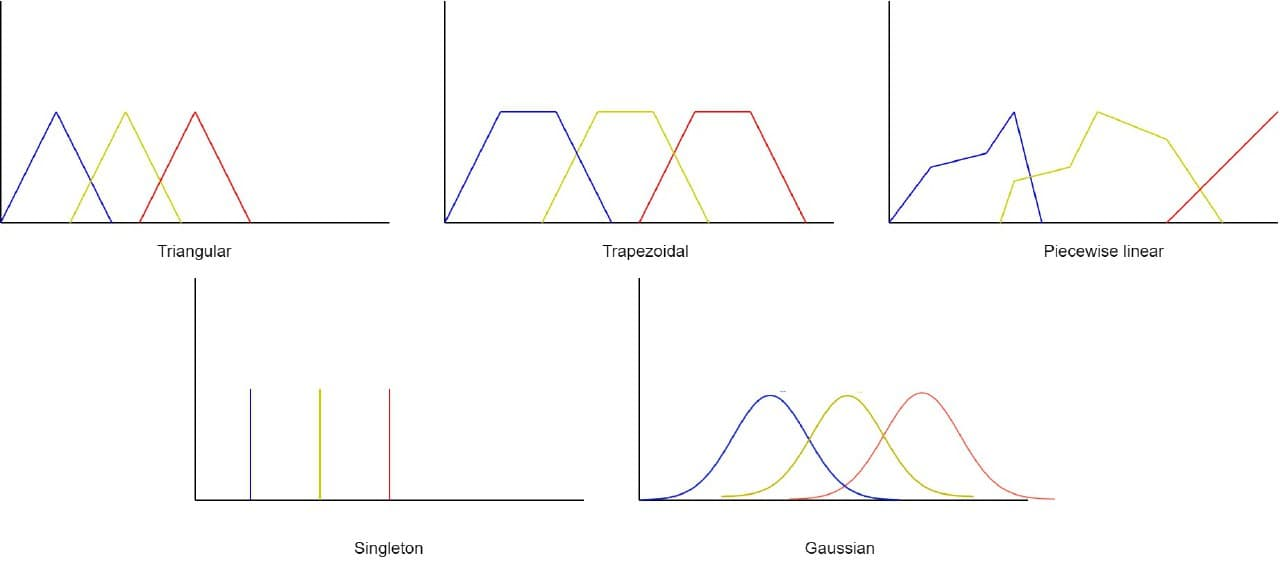
\includegraphics[width=12cm]{gfx/membership_function.png}
    \vspace{0.3cm}
    \captionsetup{justification=centering}
    \caption{Different forms of membership functions}
    \label{fig:Different forms of membership functions}
\end{figure}
\vspace*{-4mm}
We consider a multi-input-single-output fuzzy system. In health state classification normally we aim to classify a state based on the multi parameters to some specific state. The system maps $X\rightarrow Y$, where $X\subset R^{n}$ and $Y \subset R$ . As mentioned before, each fuzzy inference system consists of a fuzzifier, a fuzzy rule base, a fuzzy inference engine and a defuzzifier. Combining fuzzy inference system and neural network then we have a fuzzification layer, fuzzy rule base layer (in Mamdani Type, It called AND operation Layer), fuzzy inference layer and defuzzification layer. A fuzzifier maps $\bar{x}=\left[\bar{x_{1}},...,\bar{x_{n}}\right]\;\;\in X$ into a fuzzy set ${A}'\subseteq X$ characterized by a membership function $\mu_{{A}'}\left(x\right)$(e.g. a triangular or singleton membership function).
\\
The fuzzy rule base is a set of N fuzzy IF-THEN rules as follows:
\begin{equation}
   R^{\left ( k \right )} : \left\{\begin{matrix}
IF   & x_{1} \; is\; A_{1}^{k} & AND \\ 
     & x_{2}\; is\; A_{2}^{k} & AND \\ 
     & ...  & \\ 
     & x_{n}\; is\; A_{n}^{k} & \\
THEN & y\; is\; B^{k} & 
\end{matrix}\right. 
\end{equation} 
where
$$x=\left[x_{1},....,x_{n}\right] \in X,\,y\in Y,$$
$$A^{k}=A_{1}^{k}\times A_{2}^{k}\times ... \times A_{n}^{k}$$
are fuzzy sets characterized by membership functions $\mu_{A_{i}^{k}}\left(x_{i}\right),\;\;i=1,...,n,\;\;k=1,...,N$
and $B^{k}$ are fuzzy sets defined by membership functions $\mu_{B^{k}}\left (y\right),\;\;k=1,...,N$.
Then, the firing strength of the $k$th rule, $k=1,...,N$ is denoted as follows:
\begin{equation}
    \tau _{k}\left(\bar{x} \right )=\operatornamewithlimits{T}_{i=1}^{n}\left \{ \mu_{A_{i}^{k}}\left ( \bar{x}_{i} \right ) \right \}= \mu_{A^{k}}\left ( \bar{x} \right )
\end{equation}
Each of $N$ rules gives us a fuzzy set $\bar{B}^{k}\subseteq Y$ based on the compositional rule of inference.
\begin{equation}
    \bar{B}^{k}={A}'\circ \left(A^{K}\rightarrow B^{k}\right)
\end{equation}
Where $A^{k}=A_{1}^{k}\times A_{2}^{k}\times...\times A_{n}^{k}$ and fuzzy sets $\bar{B}^{k}$ are characterized by membership functions described by the sup-star composition:
\begin{equation}
   \mu_{\bar{B}^{k}}\left(y\right)=\operatornamewithlimits{sup}_{x \in X} \left \{ \mu_{{A}'}\left(x \right )\ast \mu_{A_{1}^{k}\times ... \times A_{n}^{k}\rightarrow B^{k}}\left(x,y \right ) \right \} 
\end{equation}
Where $\ast$ can be any operator in class t-norms (e.g. min operator $t\left( a,b\right)=min\left(a,b\right)$ or algebraic product $t\left(a,b\right)=ab$).\\
The aggregation operator for getting the fuzzy set ${B}'$ based on the fuzzy sets $\bar{B}^{k}$ is used which is the t-norm or t-conorm (e.g. $s\left(a,b\right)=max\left(a,b\right)$) depending on the type of fuzzy inference.
Finally, the defuzzifier maps from the fuzzy set ${B}'$ to a crisp point $\bar{y}$ in $Y\subset \mathbf{R}$ using COA (center of area) method as follows:
\begin{equation}
    \bar{y}= \frac{\int_{\mathbf{Y}}^{}y\cdot \mu_{{B}'}\left(y \right )dy}{\int_{\mathbf{Y}}^{}\mu_{{B}'}\left(y \right )dy}
\end{equation}
In the case of discrete systems, where $y^{-r}$ are centers of the membership functions $\mu_{B^{r}\left(y\right)}$ for $r=1,...,N$ the -crisp output $\bar{y}$ will be calculated as follows:
\begin{equation}
    \bar{y}=\frac{\sum_{r=}^{N}y^{-r}\cdot \mu_{{B}'}\left(y^{-r} \right )}{\sum_{r=1}^{N}\mu_{{B}'}\left(y^{-r} \right )}
\end{equation}
\begin{equation}
    \mu_{B}^{r}\left(y^{-r}\right)=\operatornamewithlimits{max}_{y\in\mathbf{Y}}\left\{\mu_{B^{r}}\left(y\right)\right\}
\end{equation}
\paragraph{Mamdani Neuro-Fuzzy Systems:}
In Mamdani-Type Neuro-fuzzy systems, the t-norm fuzzy implications are used (e.g. minimum or algebraic). The aggregation is performed by fuzzy union and in this case t-conorm. The fuzzy output set ${B}'\subseteq \mathbf{Y}$ using t-norm is calculated as follows:
\begin{equation}
    \mu_{{B}'}\left(y^{-r}\right)=\operatornamewithlimits{S}_{k=1}^{N}\left\{\mu_{\bar{B}^{k}}\left(y^{-r}\right)\right\}=\operatornamewithlimits{S}_{k=1}^{N}\left\{ T\left\{ \mu_{A^{k}}\left(\bar{x}\right),\mu_{B^{k}}\left(y^{-r}\right)\right\}\right\}
\end{equation}
The crisp output $\bar{y}$ is then:
\begin{equation}
    \bar{y}=\frac{\sum_{r=1}^{N}y^{-r}\cdot \operatornamewithlimits{S}_{k=1}^{N}\left \{ T\left \{ \operatornamewithlimits{T}_{i=1}^{n}\left \{ \mu_{A_{i}^{k}}\left ( \bar{x_{i}} \right ) \right \},\mu_{B^{k}}\left ( y^{-r} \right ) \right \} \right \}}{\sum_{r=1}^{N}\operatornamewithlimits{S}_{k=1}^{N}\left \{ T\left \{ \operatornamewithlimits{T}_{i=1}^{n}\left \{ \mu_{A_{i}^{k}}\left ( \bar{x_{i}} \right ) \right \},\mu_{B^{k}}\left ( y^{-r} \right ) \right \} \right \}}
\end{equation}
\paragraph{Takagi-Sugeno Neuro-Fuzzy Systems:}
This type of Neuro-fuzzy system is also known as adaptive neuro-fuzzy inference system (ANFIS) in which the rules have a fuzzy character in the IF part while the THEN part has functional dependencies. Therefore, the Rule base in ANFIS is as follows:
\begin{equation} 
\begin{split}
R^{\left(r\right)} & :\;IF \;\; \mathbf{x}\;is\;A^{r} \\
 & THEN\;\;y_{r}=f^{r}\left(x_{1},x_{2},...,x_{n}\right).
\end{split}
\end{equation}
At first we should implement fuzzy inference as follows:
\begin{equation}
    T\left(\mu_{A_{1}^{r}}\left(\bar{x_{1}}\right),\mu_{A_{2}^{r}}\left(\bar{x_{2}}\right),...,\mu_{A_{n}^{r}}\left(\bar{x_{n}}\right)\right),\;\;r=1,...,N.
\end{equation}
and then we have to compute:
\begin{equation}
    \bar{y_{r}}=f^{\left(r\right)}\left(\bar{x_{1}},\bar{x_{2}},...,\bar{x_{n}}\right),\;\;r=1,...,N
\end{equation}
and the output of ANFIS $\bar{y}$ is a normalized weighted sum of particular inputs $\bar{y_{1}},\bar{y_{2}},...,\bar{y_{N}}$:
\begin{equation}
    \bar{y}= \frac{\sum_{r=1}^{N}\bar{y_{r}}\operatornamewithlimits{T}_{i=1}^{n}\left \{ \mu_{A_{i}^{r}}\left ( \bar{x_{i}} \right ) \right \}}{\sum_{r=1}^{N}\operatornamewithlimits{T}_{i=1}^{n}\left \{ \mu_{A_{i}^{r}}\left ( \bar{x_{i}} \right ) \right \}}
\end{equation}
In the case of Takagi-Sugeno system with linear dependencies the rule base is as follows:
\begin{equation}
    \begin{split}
R^{\left(r\right)} & :\;IF \;\; \mathbf{x}\;\;is\;\;A^{r} \\
 & THEN\;\;y_{r}=c_{0}^{\left(r\right)}+c_{1}^{\left(r\right)}x_{1}+...+c_{n}^{\left(r\right)}x_{n}.
\end{split}
\end{equation}
\paragraph{Neuro-Fuzzy Systems considering Weights:}
we should distinguish between two kinds of weights regarding neuro-fuzzy systems:
(i)weights $w_{k}^{arg}\; \in \left[0,1\right], k=1,...,N$ describing the importance of each rule.\\
(ii)weights $w_{i,k}^{\tau}\in\left[0,1\right], k=1,...,N,i=1,...,n$ describing importance of antecedents or each linguistic variation of some input parameter $x_{i}$.  \\
Then we have two different rule base for each system as follows:
\begin{equation}
    R^{\left ( k \right )}:\begin{bmatrix}
IF & x_{1}\;\;is\;\;A_{1}^{k} & AND & ... \\ 
 AND& x_{n}\;\;is\;\;A_{n}^{k} &  & \\ 
 THEN& y\;\;is\;\;B^{k} &  & 
\end{bmatrix}\left ( w_{k}^{arg} \right ),
\end{equation}
\begin{equation}
    R^{\left ( k \right )}:\begin{bmatrix}
IF & x_{1}\;\;is\;\;A_{1}^{k}\left ( w_{1,k}^{\tau} \right ) & AND & ... \\ 
 AND& x_{n}\;\;is\;\;A_{n}^{k}\left ( w_{n,k}^{\tau} \right ) &  & \\ 
 THEN& y\;\;is\;\;B^{k} &  & 
\end{bmatrix}\left ( w_{k}^{arg} \right ).
\end{equation}\\\\
\textbf{Mamdani-Type and Takagi-Sugeno-Type Neuro-Fuzzy Systems Comparison:}\\
The main differences of Mamdani-Type and Takagi-Sugeno-Type neuro-fuzzy systems are as follows\cite{DBLP:journals/ijautcomp/EgajiGHY15}:\\
In Mamdani-type there is an output membership function and consequently, the output is a fuzzy set, while the output of Takagi-Sugeno-type is a constant or linear (weighted) expression. Sugeno-type is more complex in comparison to Mamdani-type, but Mamdani-type is more interpretable than the Sugeno-type.\\\\
Figure \ref{fig:Mamdani-Type Neuro-Fuzzy Architecture} shows the architecture of Mamdani-type neuro-fuzzy with 5 layers:\\\\
\textit{1.} Linear transformation layer\\
\textit{2.} Fuzzification layer\\
\textit{3.} AND-Layer where the rules are fired\\
\textit{4.} Fuzzy inference layer\\
\textit{5.} Defuzzification layer\\\\
In Takagi-Sugeno or ANFIS as shown in Figure \ref{fig:Takagi-Sugeno-Type Neuro-Fuzzy Architecture}, the two first layers are identical with the Mamdani-type neuro-fuzzy system but the third layer or rule layer is different. The IF-THEN rules in Mamdani-type are both fuzzy while in ANFIS just the IF part of rules are fuzzy and the THEN part is a function of input variables. The fourth layer of ANFIS is a normalization layer. Hence the implication method which is applied to Takag-Sugeno-type neuro-fuzzy system is the product t(a,b)=ab, the normalization layer is used to map the values of firing strength in [0,1] interval.\\ In the fifth layer, the output for each firing rule will be calculated and finally in the sixth layer, the sum of outputs of the fifth layer gives us the crisp final output of the neuro-fuzzy system.\\
\begin{figure}[H]
    \centering
    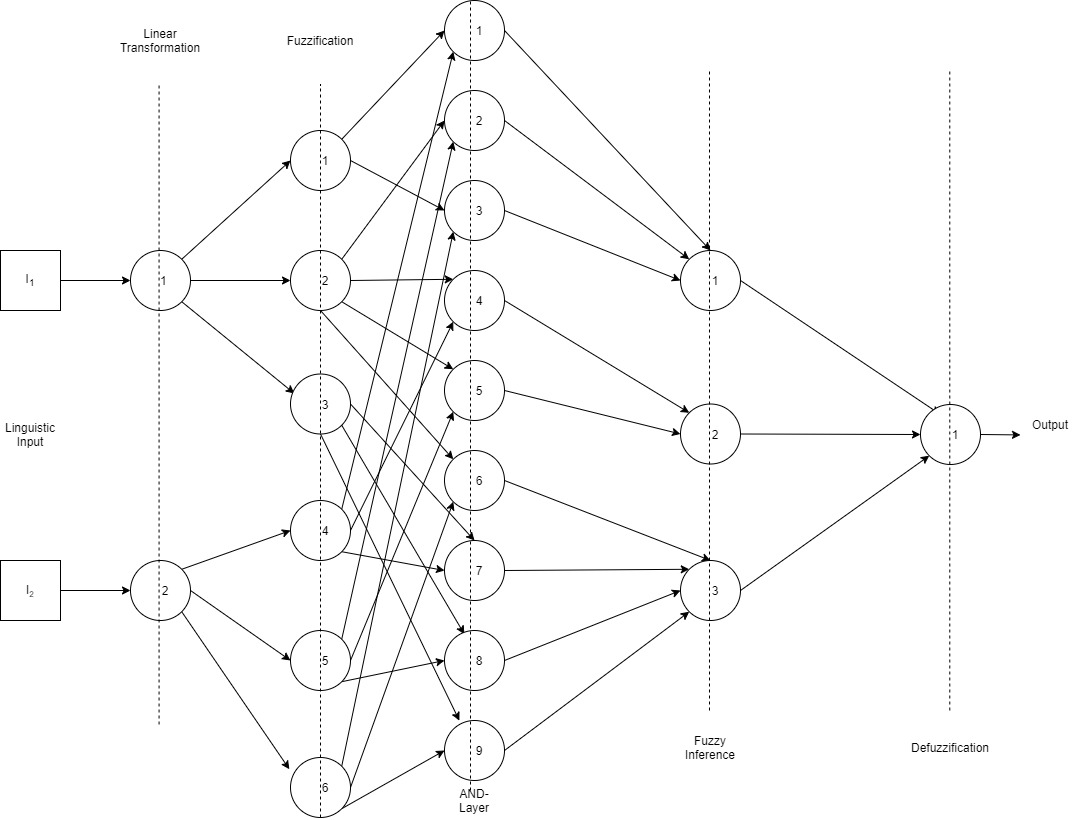
\includegraphics[width=14cm]{gfx/Untitled_Diagram.png}
    \captionsetup{justification=centering}
    \caption{Mamdani-Type Neuro-Fuzzy Architecture}
    \label{fig:Mamdani-Type Neuro-Fuzzy Architecture}
\end{figure}

\begin{figure}[H]
    \centering
    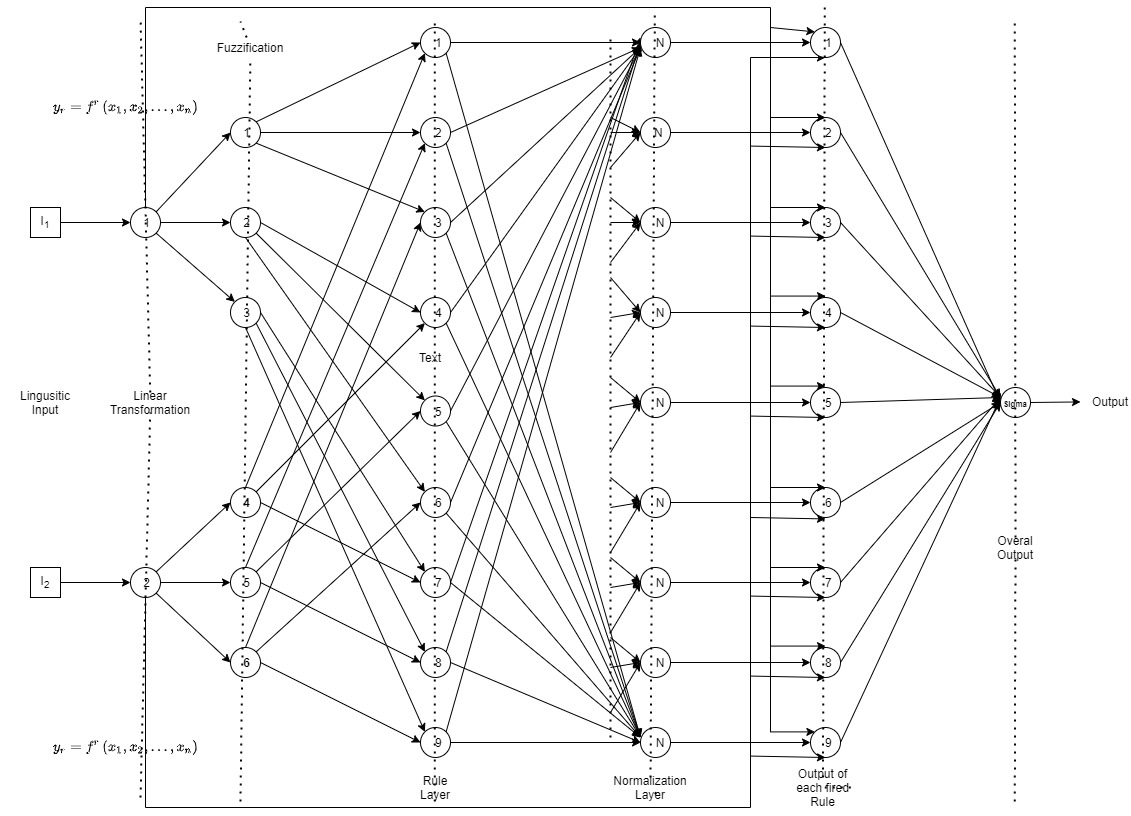
\includegraphics[width=14cm]{gfx/Takagi.png}
    \captionsetup{justification=centering}
    \caption{Takagi-Sugeno-Type Neuro-Fuzzy Architecture}
    \label{fig:Takagi-Sugeno-Type Neuro-Fuzzy Architecture}
\end{figure}


\subsection{Hidden Markov Models (HMMs)}
\vspace*{-15mm}
\hfill{\fontfamily{phv}\normalsize\emph{Saghar Heidari}}

Generally, predicting or estimating the health of a component in a mechanical system is one of the most challenges in condition based maintenance (CBM) for identifying and localizing machine failure (diagnostics). To address this problem, the Hidden Markov Model (HMM) is employed as a statistical markov model with unobserved (hidden) states for identification of the  current health state. Two kinds of regular HMM and hierarchical HMM are implemented as dynamic bayesian networks (DBNs) for health-state estimation \cite{DBLP:journals/tase/CamciC10, zhang2005integrated}.
 HMM has been used also in different fields, namely, automatic speech recognition (ASR), gen techniques, bioinformatics, handwriting recognition and partial discharges. Generally, the health-states are represented with probabilities because they can not be deterministic. The following equation shows the identified health state HS with the highest probability. Health -states affect observations, the sub-states and their transitions. Here, $X_{1:t}^{2}$ is sub-states from time 1 to $t$ and $X_{t}^{1}$ is health state at time $t$ \cite{DBLP:journals/tase/CamciC10}.
\begin{equation}
    HS=argmax_{S_{i}}(P(X_{t}^{1})=S_{i}|O_{1:t},X_{1:t}^{2})),\forall \;i,\;  i=1 ,\,2, \cdots ,N
\end{equation}
HMM uses time-series data that develop by a finite number of states which are hidden to outside observers and depend on the predecessor states. It is a process that produces a sequence of observable symbols as an output.
It consists of double stochastic processes:  A markov chain for the transition from one state to another in the hidden layer and the stochastic visible output in the observable layer. 

\subsubsection*{HMM Elements:}
HMM consists of several parameters \cite{camci2005dynamic, DBLP:journals/tase/CamciC10} that are listed as below :
\begin{enumerate}
    \item The state space S with N number of hidden states, $S=\left \{ S_{1},S_{2},\cdots,S_{N} \right \}$.\vspace*{-3mm}
    \item The set of observations is denoted as  
    $O=\left \{ O_{1},O_{2},\cdots,O_{T} \right \}$ which T is the number of observations in the sequence and $O_{t}$ denotes observations at time $t$. $O_{t}$ might be a discrete symbol  as $O_{t}\in \left \{ 1,\cdots ,L \right \} $ or a feature vector from L dimensional space , $O_{t}\in \mathbb{R}^{L} $.
    There exists also state sequence $X=\left \{ X_{1},X_{2},\cdots,X_{T} \right \}$  and $X_{t}$ is defined as health state at time $t$.\vspace*{-3mm}
    \item Transition matrix of state transition probability distribution expressed as $ A=\left \{  a_{ij}\right \}=P(X_{t}=S_{i}|X_{t-1}=S_{j})$ , $1\leq i,j\leq N$ which shows the probability of being in state $S_{i}$, at time t given that it is in state $S_{j}$ in time $t-1$.\vspace*{-3mm}
    \item Emission probability is called also observation probability distribution, $B=\left \{  b_{j}\left ( k \right )\right \}=P(O_{t}=k|X_{t}=S_{i}))$,  $1\leq i\leq N$ which defines the probability of observing k at time t given the state i.\vspace*{-3mm}
    \item The initial state distribution is the probability of being in state i when t=0 and is shown as $ \pi \left ( i \right )=P\left ( X_{1}=S_{i} \right )$ ,  $1\leq i\leq N$.
\end{enumerate}
    
The compact notation $\lambda =\left \{ A,B,\pi  \right \}$  for HMM is employed to show the complete parameter of model. Figure \ref{fig:HMM structure} shows the HMM structure.
\newline

\begin{figure}[H]
	\centering
	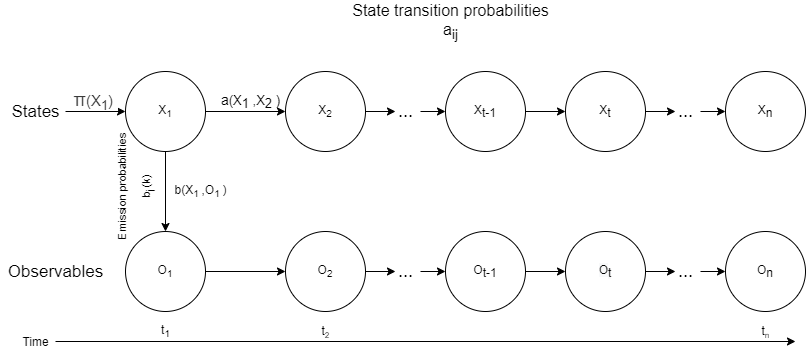
\includegraphics[width=12cm]{gfx/HMM.png}
    \captionsetup{justification=centering}
	\caption{Structure of Hidden Markov Model}
	\label{fig:HMM structure}
\end{figure}

\subsubsection*{HMM Problems:}
There are three main problems that can be solved by this model. These problems are the following:
\begin{enumerate}
\item{Evaluation Problem:}\\
The probability of the observation sequence  $O=\left \{ O_{1},O_{2},\cdots,O_{T} \right \}$ and  $\lambda =\left \{ A,B,\pi  \right \}$ is given.
The easiest way to calculate $P(O|\lambda )$ is the Brute-Force approach. Every state sequence of length $T$ is counted and the probability of each state sequence X given the model is calculated. First, hidden states denoted as $X=\left \{ X_{1},X_{2},\cdots,X_{T} \right \}$. Then, the emission probability B and transition matrix A, $\pi $ are used.
This approach solves the evaluation problem but it is too costly. The better way is the forward-backward (FB) algorithm \cite{DBLP:conf/interspeech/Bilmes98}, which is more efficient than direct evaluating. It uses forward variable $a_{t}(i)$ defined as
$a_{t}(i)= P( O_{1},O_{2},\cdots,O_{t} ,X_{t}=S_{i}|\lambda )$ which is the probability of partial observation sequence until time t and the state $S_{i}$ at step t given the model.\vspace*{-3mm} 
\item{Decoding Problem:}\\ The most likely state sequence that might produce the observation sequence is determined by using the Baum–Welch algorithm or the expectation maximization (EM) algorithm which utilizes both the forward and backward procedures \cite{DBLP:conf/icassp/Poritz88}.\vspace*{-3mm}
\item{Training Problem:}\\ The EM algorithm is used for solving the problem of adjusting the model parameters   $\lambda =\left \{ A,B,\pi  \right \}$   to maximize the likelihood of the observation sequence $P(O|\lambda )$).
\end{enumerate}

\subsubsection*{Implementation of HMM:}
The first step is to build an HMM for each state. For creating HMMs, it should be decided whether one HMM is used or a set of HMMs. Each state will represent a different health state when we have one HMM but in a set of HMMs, each HMM will be trained to express a different health state.
Then, a data sequence (observation sequence) is selected and the log-likelihood probability of obtaining this observation sequence given the HMM model is calculated for all HMMs $P(O|\lambda )$ through the FB algorithm. The HMM model with the highest log-likelihood value is selected as the best candidate for representing the health state and is allowed to further learn by using the current health state. Training continues until reaching the desired number of iterations for convergence. For testing, a test sequence as input is given to several trained HMM to compute the log-likelihood probabilities. The HMM model with the highest log-likelihood value is selected as the best candidate for representing the health state.
\paragraph{Dynamic Bayesian Network (DBN):}
It is an extension of bayesian network (BN) for modeling a system that is changing dynamically over time. DBN \cite{camci2005dynamic, DBLP:journals/tase/CamciC10} is designed to model probability distributions over sequence of random variables. It can handle sequenced observations that are generated by some hidden states evolving in time. DBN consists of two networks: a prior network which shows the prior probabilities of all variables in the network when $t = 0$ and a transition network which shows the probabilities of all the variables when $t = 1,2,...n$.
\paragraph{Dynamic Bayesian Network implementation of HMM:}
DBN shows the hidden-state as a set of random variables, while HMM has a single discrete random variable. DBN has two levels: observation level and hidden-state level \cite{camci2005dynamic}.
First, hidden-state $X_{t}$ and previous observation $O_{t-1}$ generate observation in time $t$ denoted as $O_{t}$. Then, a conditional probability distribution of each node given its parents is defined during the training process. These consist of initial probability distribution $P(X_{1}=i)$  , state transition distribution $P(X_{t}|X_{t-1})$, and the observation distribution $P(O_{t}|X_{t})$. Here, the observation distribution is considered as continuous and Gaussian:
\begin{equation}
P(O_{t}|X_{t}=i)\sim N(\mu_{i},\sigma _{i}^{2})
\end{equation}
As shown in Figure \ref{fig:DBN representation of HMM}, there are two different nodes in the hidden state level ($X_{1}$,$X_{t}$) in all-time slices $(t=1,2,...n)$ instead of M number of nodes. All the observations are represented by one node (O) since they have the same parent ($X_{t}$).
The purpose of a DBN performing as an HMM is to deduce the hidden-state given the observation sequence which is shown as $P(X_{t}=i|O_{1:t})$.
\begin{figure}[H]
	\centering
	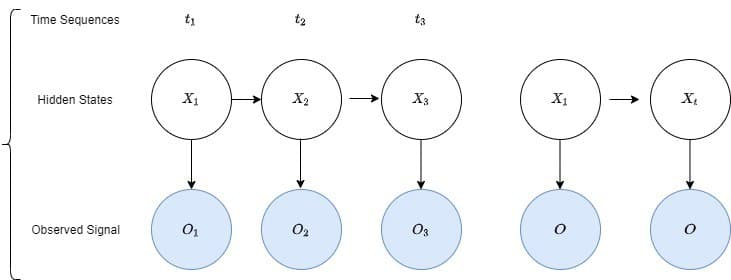
\includegraphics[width=10cm]{gfx/DBN_representation_of_HMM.png}
    \captionsetup{justification=centering}
	\caption{DBN representation of HMM}
	\label{fig:DBN representation of HMM}
\end{figure}

\subsubsection*{Hierarchical Hidden Markov Models:}
Hierarchical HMM (HHMM) is an extension of an HMM for modeling hierarchical structures for sequential data \cite{camci2005dynamic, DBLP:journals/tase/CamciC10}. Here, states include sub-states and both sub-states
and states. In an HHMM, the states also can produce single observations (production states) or strings of observations (abstract states). For instance, hidden states consist of the $t-th$ top-state denoted as  $X_{t}^{1}$ and  $X_{k}^{2}$ represents the $k-th$ sub-state. The transition between hidden states in the same level is horizontal transition. After sub-state transitions reach the last state, the health state transition occurs which is called vertical transition. Estimating the HHMM elements and model structure is more complex than HMM. DBN helps to represent HMMs in an efficient way by adding the flexibility of implementing different kinds of HMM like HHMM.

\paragraph{Dynamic Bayesian Network implementation of HHMM:}
In Figure \ref{fig:DBN representation of HHMM} , there is one arrow between the hidden-states in the top,  sub-state levels and the observation. There is also one arrow between top-level states and the sub-level state. When top-states for each sub-state is replicated, it makes a problem of losing the hierarchical structure. A binary control variable $F$ is used for solving this issue. If $F=1$, a top-level state changes and the lower-level state reaches its last possible state.
\begin{figure}[ht]
	\centering
	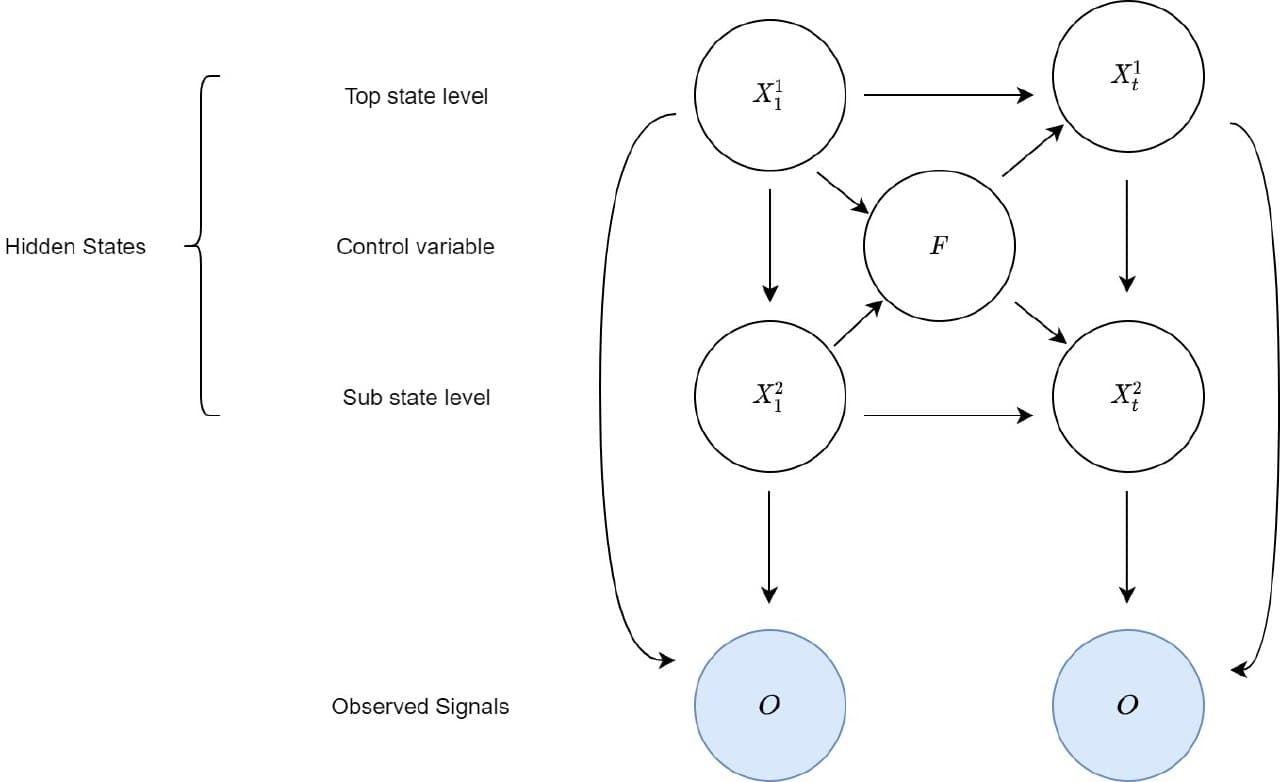
\includegraphics[width=10cm]{gfx/DBN_representation_of_HHMM.png}
    \captionsetup{justification=centering}
	\caption{DBN representation of HHMM}
	\label{fig:DBN representation of HHMM}
\end{figure}
The conditional probabilities of variables in the initial
time slice are initial distributions and are represented as:
\begin{equation}
    P(X_{1}^{1}=j)=\pi ^{1}(j)
\end{equation}
\begin{equation}
    P(X_{1}^{2}=i|X_{1}^{1}=j)=\pi_{j}^{2}(i)
\end{equation}
where $\pi ^{1}(j)$ is the initial top-level state distribution. When the upper state is in state $j$, the probability of sub-state being in state i denoted as $\pi_{j}^{2}(i)$. In this work, we have a vertical transition if $F=1$, otherwise we have a horizontal transition.
 The conditional probability distribution is shown in the next equation. Here, $A^{1}(i,j)$ is the top-level state transition probability from top state $i$ to $j$ if $F=1$.
\begin{equation}
P(X_{t}^{1}=j|X_{t-1}^{1}=i,F_{t-1}=f)=\begin{cases}
1 ,& \text{ if } f=0 , i=j \\ 
0, & \text{ if } f=0 , i\neq j \\ 
A^{1}(i,j),& \text{ if } f= 1
\end{cases}
\end{equation}
 In the sub-state level, the conditional probability in the sub-state level is based on either the initial distribution or the transition distribution depending on $F$.
\begin{equation}
 P(X_{t}^{2}=j|X_{t-1}^{2}=i,F_{t-1}=f,X_{t}^{1}=k)=\begin{cases} 
A_{k}^{2}(i,j),& \text{ if } f= 0 \\ 
\pi_{k}^{2}(j) ,& \text{ if } f=1 \\ 
\end{cases}
\end{equation}
If the high-level state is in $k$, the transition probability from state $i$ to $j$ is $A_{k}^{2}(i,j)$ and the initial sub-state level distribution is $\pi_{k}^{2}(j)$. The probability
of turning $F$ “on” ($F=1$) is equal to the probability of transition to the last state $l$.
\begin{equation}
    P(F_{t}=1|X_{t}^{1}=k,X_{t}^{2}=i)= A_{k}^{2}(i,l)
\end{equation}
The conditional distribution of the observed state is shown in next equation,
\begin{equation}
P(O_{t}|X_{t}^{1}=i,X_{t}^{2}=j)\sim N(\mu _{i,j},\sigma _{i,j}^{2})
\end{equation}



\subsection{K-Nearest Neighbors model (KNN)}
\vspace*{-12mm}
\hfill{\fontfamily{phv}\normalsize\emph{Saghar Heidari}}

K-Nearest Neighbors model is a non-parametric machine learning model that is used for classification and regression problems. This multi-class algorithm is also used for identifying the health condition of a system \cite{hasan2020health}. KNN works based on a similarity measure (minimum distance) and has two phases: 
In the training phase, the nearest neighbors are determined(see below in the KNN algorithm ). In the testing phase, predicted classes are compared to given class labels of test data. The goal of this approach is to predict the class for new input data based on the classes of available training data.
The KNN Algorithm employs distance measures like the standard Euclidean distance, Manhattan, and Minkowski distance. These metrics are used to find the nearest neighbors of an observation which is classified by its K nearest neighbors and the distances. The equation for calculating distance of two points
($X=\left \{ x_{1},x_{2},...,x_{n} \right \}$, $Y=\left \{ y_{1},y_{2},...,y_{n} \right \}$) with n elements is shown as below:
\begin{itemize}
\item  Euclidean distance : 
\begin{equation}
D(X,Y)=\sqrt{\sum_{i=1}^{n}}(x_{i}-y_{i})^{2} 
\end{equation}
\vspace*{-4mm}
\item  Manhattan distance: 
\begin{equation}
    D(X,Y)=\sum_{i=1}^{n}\left | x_{i}-y_{i} \right |
\end{equation}
\vspace*{-4mm}
\item Minkowski distance:
\begin{equation}
D(X,Y)=\left (\sum_{i=1}^{n}\left | x_{i}-y_{i} \right | ^{q} \right )^{1/q}
\end{equation}
\vspace*{-4mm}
\end{itemize}
\subsubsection*{KNN algorithm:}
The algorithm of KNN works as follows:
\begin{enumerate}
    \item Select the value k which determines how many nearest neighbors should be considered.
    \vspace*{-3mm}
    \item Calculate the distance between new input data and training samples via a distance function as defined above.
    \vspace*{-3mm}
    \item Sorting out the calculated distance in ascending order.
    \vspace*{-3mm}
    \item Choose k nearest neighbor from the sorted list.
    \vspace*{-3mm}
    \item Assign a class to the new data point which is a majority among its neighbors.
    \vspace*{-3mm}
\end{enumerate}
Figure \ref{fig:Example of KNN algorithm} shows the example of the KNN algorithm, in which the new sample is classified based on its neighbors. 


\begin{figure}[H]
	\centering
	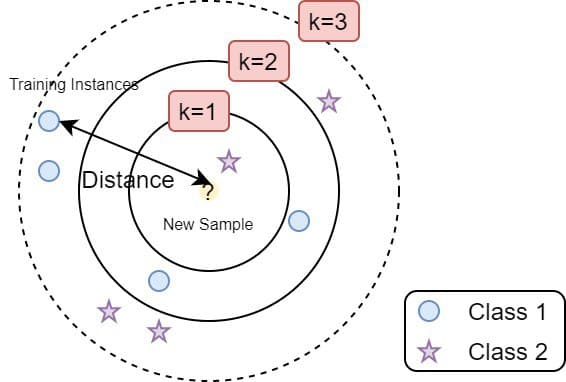
\includegraphics[width=8cm]{gfx/KNN.png}
    \captionsetup{justification=centering}
	\caption{Example of KNN algorithm}
	\label{fig:Example of KNN algorithm}
\end{figure}



\section{Evaluation setup}

\label{sec:system:sec5}

There are two main aspects that should be considered in the evaluation of a model. First, the model parameters by which the model performs at its best, which is also known as Hyperparameter tuning. Second, the performance of the model or how good is the model in predicting the target values (e.g. accuracy of the model).

\subsection{Score based evaluation metrics}
\vspace*{-12mm}
\hfill{\fontfamily{phv}\normalsize\emph{Saghar Heidari}}

To evaluate a classification model, there are some aspects that should be considered. First, The number of classes in the model. If we have to deal with a binary classification model or a multi-class classification model. Second, the distribution and importance of classes, which means if the data points for different classes are almost the same or most of the data points are classified for some specific class (balanced or imbalanced datasets). Whether the classes are equally important or some specific class is more important than the others. Based on such considerations, while an evaluation metric can describe some specific model precisely at the same time the same metric can be misleading for another model. In the following, we describe the well-known and well-established evaluation metrics and the usefulness of each for different classification tasks \cite{DBLP:journals/prl/FerriHM09, hasan2020health}.

\paragraph{Confusion Matrix:}
It is a Matrix that compares actual values of the target parameter and the predicted values for instance in the case of binary classification the confusion matrix consists of 4 categories as follows \cite{DBLP:journals/corr/BrancoTR15, article}:
\begin{enumerate}
\item{True Positive (TP):} the class is predicted as a class (+) and the actual class is (+). \vspace*{-6.5mm}
\item{False Positive (FP):} the class is predicted as a class (+) but the True class is (-). \vspace*{-6.5mm}
\item{True Negative (TN):} the class is predicted as a class (-) and the actual class is (-). \vspace*{-6.5mm}
\item{False Negative (FN):} the class is predicted as a class (-) but the actual class is (+).
\end{enumerate}

\paragraph{Normalized Confusion Matrix:}
Calculates the percentage of each category regarding a total number of predictions e.g. if the number of prediction is N=(TP+FN+FP+TN) then:
\begin{enumerate}
    \item $0\leq \frac{TP}{N} \leq 1$ \vspace*{-3mm}
    \item $0\leq \frac{FP}{N} \leq 1$ \vspace*{-3mm}
    \item $0\leq \frac{TN}{N} \leq 1$ \vspace*{-3mm}
    \item $0\leq \frac{FP}{N} \leq 1$ \vspace*{-3mm}
\end{enumerate}
\paragraph{Accuracy:}
It is defined as the number of correctly predicted values divided by the total number of all values. Using confusion matrix in binary classification we can define accuracy as follows:
\begin{equation}
    Accuracy= \frac{TP+TN}{TP+TN+FP+FN} 
\end{equation}

\paragraph{Precision:}
The percentage of correctly predicted positive class out of all positive predicted values.
\begin{equation}
Precision = \frac{TP}{TP+FP}    
\end{equation}

\paragraph{Recall:}
Recall also known as sensitivity in medical science and true positive rate.
The number of correctly predicted positive class (+) divided by the number of values in the positive class.
\begin{equation}
   Recall\;(TP_{rate}) = \frac{TP}{TP+FN}
\end{equation}
\paragraph{Specificity:}
It is the number of correct predictions of the negative class (-) or TN divided by the actual number of values in the negative class.
\begin{equation}
    Specificity\;(TN_{rate})=\frac{TN}{TN+FP}
\end{equation}
The following equation shows the calculation of False Positive Rate (FPR).
\begin{equation}
    FP_{rate}=\frac{FP}{TN+FP} 
\end{equation}

\paragraph{F1-Score:}
This score considers both precision and recall simultaneously and hence computes the harmonic mean of precision and recall as follows:
\begin{equation}
    F1-Score = 2\times \frac{Recall\times  Precision}{Recall+  Precision}
\end{equation}
\paragraph{ROC and AUC:}
The Receiver Operator Characteristic (ROC) and the Area Under The Curve (AUC) curve are evaluation metrics for checking the performance of classification problems.
ROC is plotted by TPR against FPR (on axis y and x respectively). The more the curve shifted toward the left top corner, the better the model can distinguish between two groups and the more the curve shifted toward indifferent or arbitrary line (the diagonal where x=y), the weaker is model in differentiating between two groups. The greater is the AUC or the area under the ROC curve, the model is better.

\paragraph{Metrics for multiclass classification:}
In this case for the calculation of metrics like precision and recall and F1-Score, we should use the principle of one-against-others which means each time we consider a class as a positive class and the other classes as a negative class and repeat it for all classes. Then, the calculation of metrics would be as same as for binary classification.
There are 3 more metrics for multiclass classification problem as follows \cite{grandini2020metrics}:
\begin{enumerate}
\item Micro-F1: Micro average considers total values of TP, FP, FN regardless of which class they belong to and then computes precision, recall as well as F1-Score as expected the values of precision and recall and Micro-F1 are same.
\item Macro-F1: It computes F1-scores of each class and then take unweighted average of them (without consideration of the number of each class). 
\item Weighted-F1: It takes the frequency of each class into account.
Applying the same principle (binarization of a multiclass classification), the Roc curves for a multi class classification can be obtained.
\end{enumerate}
\paragraph{Balanced and imbalanced data:}
In health state classification, we normally deal with imbalanced datasets. In most cases, the majority of data points represent the normal or healthy class and the classes have different levels of importance. Classes that represent sudden failure are more important than classes that represent gradual failures.
One common approach for binary classification is to tag minority class as positive class and then calculate some metrics as sensitivity or specificity \cite{DBLP:journals/corr/BrancoTR15, article}.

\textit{1. F-Beta-Score:} F1-score is one of the popular metrics for imbalanced classes but as the importance of false Positive and false negatives can be different, the F-Beta-Score is introduced, in which different weights will be assigned for false positives and false negatives. For instance, F-0.5-Score and F-2-Score give more weights for positive class and negative class respectively.
\begin{equation}
 F_{\beta } =\frac{(1+\beta ^{2})\cdot (precision\cdot recall )}{(\beta ^{2}\cdot precision+ recall)}
\end{equation}
\textit{2. Precision-Recall Curve:} This is another metric that is quite similar to the ROC curve but is useful in the case of imbalanced data. Precision-Recall curves have the recall and precision rates expressed on the axes. The precision on the y-axis plotted against Recall on the x-axis. The better classifiers tend to right top corner and the arbitrary classifiers is a horizontal line (y=0.5). The area under Precision-Recall curve as AUROC curve (Area Under the Receiver Operating Characteristics) can be used for comparison of different classifiers.



\subsubsection{Calibration scores}
\vspace*{-12mm}\hfill{\fontfamily{phv}\normalsize\emph{Anurose Prakash }}

In most of the cases of supervised health state estimation, the health state is assigned based on the probabilistic models. These models yield a probability membership of a data sample to each of the possible class groups in the problem, $\widehat{p}(c|x)$. By setting a discriminatory threshold, it is possible to select one of the class assignments. However, the evaluation of the classification process by means of standard scores (Accuracy, Recall, etc.) disregards the information about the uncertainty in-class assignment. By contrast, calibration scores aim to measure how close the probability assignment given by the classifier is from the true distribution of the class. Thus, calibration scores incorporate classifier uncertainty in the assessment of the classification performance. Among the best-known calibration scores for classification is the Brier score, which is defined as:

\begin{equation}
BS = \frac{1}{N} \sum_{i=1}^N \sum_{j= \{c^+, c^-\}}(\widehat{p}(C = j|x^{(i)} - \delta(j,c^{(i)}))^2  
\end{equation}
where $\widehat{p}(C = j|x^{(i)})$ is the probability assigned by the classifier to the $i^{th}$ instance for class group $j$ and $\delta(j, c(i))$ is a Kronecker delta which equals 1 if the class
label for the $i^{th}$ instance is $j$ and 0 otherwise. Therefore, the Brier score is useful in problems where the interest lies in fitting the data distribution or in problems where experts perform class assignments on the basis of the expected probability class membership. Similarly, another well-known score used in calibration is the log loss:
\begin{equation}
Log Loss = \frac{1}{N} \sum_{i=1}^N \sum_{j= \{c^+, c^-\}} \delta(j,c^{(i)}) \log_2(\widehat{p}(C = j|x^{(i)}))
\end{equation}


\subsection{Generalization from binary to multi-class classification problems}
\vspace*{-12mm}
\hfill{\fontfamily{phv}\normalsize\emph{Anurose Prakash}}\newline

Evaluation metrics such as accuracy, classification error, Brier score and log loss can be straightforwardly extended to problems with multiple class labels. But, this is not the case with other scores
(e.g. recall, precision, etc.) and graphical methods (e.g. ROC curves, lift graphs,
etc.) as they can not be used directly in multi-class problems because they are based on
the presence of only two classes: positive and negative \cite{article}. Hence, the generalization schemes are used to reduce multi-class problems to a set of binary classification problems in order to use the presented scores in multi-class problems. Such
generalization schemes are OVA (one vs. all) and OVO (one vs. one).
\paragraph{OVA:}
Given that the class variable can take $r_C$ values, for each one of these binary problems is assigned a class value ($c_i$ with $i$ = 1,...,$r_C$) as the positive class and the rest of the class values are considered to belong to the negative class. Hence, $r_C$ scores (one for each binary classification problem) are produced denoted as $S_i$ with $i$ = 1,...,$r_C$ and the OVA score is obtained as follows:
\begin{equation}
    S_{OVA} = \sum_{i=1}^{r_C} p(c_i) . S_i
\end{equation}
\paragraph{OVO:}
Given that the class variable can take $2^{r_C}$ values, for each problem only those samples assigned to $c_i$ and $c_j$ class labels are considered with $i, j$ = 1,...,$r_C$ and $i < j$). Thus, $c_i$ is taken as the positive class and $c_j$ as the negative class to calculate the score, $S_{i,j}$ . Finally, the score is calculated as follows:
\begin{equation}
    S_{OVO} = \frac{1}{2^{r_C}}\sum_{i=1}^{r_C-1}\sum_{j=i+1}^{r_C} S_{i,j}
\end{equation}
%\begin{figure}[htb]
%	\includegraphics[width=\textwidth]{gfx/Clean-Thesis-Figure}
%	\caption{Figure example: \textit{(a)} example part one, \textit{(c)} example part two; \textit{(c)} example part three}
%	\label{fig:system:example1}
%\end{figure}

%\Blindtext[1][2]

% \section{System Section 2}
% \label{sec:system:sec2}

% \Blindtext[1][2]

% \begin{figure}[htb]
% 	\includegraphics[width=\textwidth]{gfx/Clean-Thesis-Figure}
% 	\caption{Another Figure example: \textit{(a)} example part one, \textit{(c)} example part two; \textit{(c)} example part three}
% 	\label{fig:system:example2}
% \end{figure}

% \Blindtext[2][2]

% \section{System Section 3}
% \label{sec:system:sec3}

% \Blindtext[4][2]

% \section{Conclusion}
% \label{sec:system:conclusion}

% \Blindtext[2][1]
           % INCLUDE: health state classification
% !TEX root = ../main.tex
%
\chapter{Health Index Estimation}
\vspace*{-15mm}\hfill{\fontfamily{phv}\normalsize\emph{Selami Hoxha and Gourav Prakash}}
\label{sec:hi_estimation}

\cleanchapterquote{Estimating is what you do when you don't know.}{Sherman Kent}{(Yale University professor)}

% \Blindtext[2][1]
This chapter introduces Health Index (HI) as an important tool for performing predictive maintenance. First, we
present the motivating factors for constructing a HI and its role in predictive maintenance in section \ref{sec:hi_estimation:motivation}.
The formal definition of the HI is given in section \ref{sec:hi_estimation:formal_definiton}. In section
\ref{sec:hi_estimation:datasets} there are presented three publicly available datasets that are used for training
and evaluating the approaches presented in section \ref{sec:hi_estimation:approaches}. Section
\ref{sec:hi_estimation:approaches} contains six different approaches in detail. The approaches are based on
current research on machine learning algorithms and techniques for performing predictive maintenance. The
presented approaches are General Regression Neural Network (GRNN), Artificial Neural Networks (ANN), Ensemble
methods, LSTM Encoder Decoder, Hierarchical Gated Recurrent Unit (HGRUN) and Kullback-Leibler Divergence. Finally,
in section \ref{sec:hi_estimation:evaluation} evaluation metrics are presented.


\section{Motivation}
\vspace*{-15mm}\hfill{\fontfamily{phv}\normalsize\emph{Gourav Prakash}}
\label{sec:hi_estimation:motivation}

The world is moving towards an era of technology where machine performance takes precedence over labor. There are
many drawbacks to this development, including a large amount of data and different types of machines that must be
updated to avoid certain bugs that can cause a huge loss of resources and financial support. Predictive maintenance
plays an important role in solving this problem. The predictive maintenance strategy can estimate the current state
of the system and predict the future state of the system. There are many techniques that can be used to predict
system operating conditions. One of these techniques is the Health Index (HI). It estimates the current state of
the system and monitors it over a period of time. The HI estimates the health of
the system by setting its state between 0 and 1, with a value closer to 1 indicating that the system is in good
condition, while a value closer to 0 indicates a system failure.

% Over the past few decades, the HI has become an increasingly 
% popular tool for predictive maintenance strategies. 
% Using the HI as an estimator can help estimate the state 
% of the system.where (i.e., 100\%) 
% means the system is in good health while 0 (i.e., 0\%) means system 
% failure. These values ​​can be shown graphically
% as a deterioration curve. By drawing these data over
% a specific timestamp, histories of the data
% collected can be created.

% \Blindtext[2][2]

\newpage
\section{Formal problem definition}\label{sec:Fpd_HI}
\vspace*{-15mm}
\hfill{\fontfamily{phv}\normalsize\emph{Gourav Prakash}}
\label{sec:hi_estimation:formal_definiton}

The health index is a state assessment index that acts as an approximation  of the current health of the system. The
health index of the system is a value that ranges between 0  and 1. A value close to 1 represent a healthy system,
and a value close to 0 indicates an unhealthy system or complete system failure.

The health index estimator $h$ maps the historical sensor data to health index values.  Formally, given data $x\in X$
we learn an estimator $ h : X \rightarrow Y $, which predicts the health index $y$ of a system. The input space $X$
contains of time series data as mentioned in section \ref{sec:intro:time-series-definition}. The output $y \in Y$ is
the estimated health index, where the output space $Y = [0,1] $.

To learn a health index estimator, we use training data from the set $D_{train}$ which contains $N$ instances of the
time series data denoted by $x_i$. The training data is of the form
\begin{equation}
    D_{train} = \{x_i\}_{i=1}^N.
\end{equation}
To evaluate the performance of the HI estimator, we use the test set
which has the form
\begin{equation}
    D_{test} = \{(x_i,y_i)\}_{i=1}^M ,
\end{equation}
where $y_i$ is the corresponding HI value for the instance
$x_i$.
% \\\\The performance of HI estimator for test data is measured using a loss
% function.
% \begin{equation}
%     \mathcal{L}(D_{test}) =\frac{1}{N} \Sigma_{i=1}^N 1-\sigma_i
% \end{equation}


% \Blindtext[3][2]

\newpage
\section{Publicly Available Datasets}
\vspace*{-15mm}
\hfill{\fontfamily{phv}\normalsize\emph{Selami Hoxha}}
\label{sec:hi_estimation:datasets}

In this section three datasets are presented. The milling dataset was created by performing lab experiments on
a milling machine \cite{millingData}. The bearing dataset was also created on a lab experiment where a motor
and a rotating shaft with four bearings was used \cite{bearingData}. The air quality dataset was created in a
field where different air quality factors were measured \cite{airQualityData}.

\subsection{Milling Dataset}
\label{sec:hi_estimation:datasets:milling_dataset}

The milling dataset \cite{millingData} is a created by performing lab experiments in a milling machine. The
experiments are run-to-failure experiments. The main purpose of the experiment is tool wear investigation. The
tool wear is measured under various operating conditions, where the conditions of the experiment are determined
by the fields DOC (depth of cut), feed (sideway cut), and type of material. Each of these fields has 2 settings,
which gives a total of 8 possible settings in which the machine was run. The depth of cut can be 1.5mm or
0.75mm; feed can be 0.5mm\textbackslash rev or 0.25mm\textbackslash rev (rev for revolution); the material is 1
for cast iron and 2 for steel. For each of the 8 settings the experiment was run 2 times, where each of the runs
is marked with a case number from 1 to 16, and is recorded in the field "case". In the experiment sensors for
measuring the current of the spindle, the vibration of spindle and table, and the acoustic emission of spindle and table
were setup. The dataset is organized in a ".mat" file and contains an array of 167 structs. Each struct contains
the 13 fields. The sensor measurements are recorded on arrays of type double with 9000 elements, and are recorded
in the fields smsAC, smsDC, vib\_table, vib\_spindle, AE\_table and AE\_spindle. Table
\ref{sec:hi_estimation:datasets:milling_table} shows all the fields and their description.

\begin{table}[ht]
    \centering
    \begin{tabular}{| l | l | }
        \hline
        \textbf{Field Name} & \textbf{Description}                        \\
        \hline
        case                & case number (1-16)                          \\
        \hline
        run                 & number of runs                              \\
        \hline
        VB                  & flank wear, was not measured after each run \\
        \hline
        time                & duration of experiment                      \\
        \hline
        DOC                 & depth of cut                                \\
        \hline
        feed                & feed                                        \\
        \hline
        material            & material                                    \\
        \hline
        smcAC               & AC current of spindle                       \\
        \hline
        smcDC               & DC current of spindle                       \\
        \hline
        vib\_table          & table vibration                             \\
        \hline
        vib\_spindle        & spindle vibration                           \\
        \hline
        AE\_table           & table acoustic emission                     \\
        \hline
        AE\_spindle         & spindle acoustic emission                   \\
        \hline
    \end{tabular}
    \vspace{0.3cm}
    \captionsetup{justification=centering}
    \caption{Fields and their description of milling dataset}
    \label{sec:hi_estimation:datasets:milling_table}
\end{table}




\subsection{Bearing Dataset}
\label{sec:hi_estimation:datasets:bearing_dataset}

The bearing dataset \cite{bearingData} consists of three datasets. Each dataset is collected from performing a
respective test-to-failure experiment. The experiments are performed in the same setup, but using different number
of sensors. The experiment is setup with a motor that rotates a shaft, and the shaft has four bearings. For
creating set 1 two accelerometers were used for each bearing, meanwhile for set 2 and 3 one accelerometer for each
bearing is used. In each experiment the data is collected every 10 minutes for 1 second with a frequency of 20kHz
(except for dataset 1 in which the first 48 recordings are done every 5 minutes). Every file consists of 20480 data
points which have eight columns for set 1 and four columns for set 2 and 3, which correspond with the number of
sensors in each experiment. The name of the file is the time step when the measurements are made. A summary of
these datasets is given in table \ref{sec:hi_estimation:datasets:bearing_table}.

\begin{table}[ht]
    \centering
    \renewcommand{\arraystretch}{2}
    \begin{tabular}{| l | l | l | l | }
        \hline
        \textbf{Set number} & \textbf{Columns} & \textbf{Number of files} & \textbf{Reason for failure} \\[0.2cm]
        \hline
        1                   & 8                & 2156                     &
        \parbox{6cm}{Bearing 3 had an inner race defect                                                 \\ Bearing 4 had a roller element defect}       \\[0.2cm]
        \hline
        2                   & 4                & 984                      &
        Bearing 1 had an outer race failure                                                             \\
        \hline
        3                   & 4                & 6324                     &
        Bearing 3 had a outer race failure                                                              \\
        \hline
    \end{tabular}
    \vspace{0.3cm}
    \captionsetup{justification=centering}
    \caption{Bearing datasets short description}
    \label{sec:hi_estimation:datasets:bearing_table}
\end{table}


\subsection{Air Quality Dataset}
\label{sec:hi_estimation:datasets:air_quality_dataset}

Air quality dataset \cite{airQualityData} authored by Saviero De Vito was developed in a 13 month period which resulted in
9358 instances. The data was gathered in a field in a polluted area in Italy. The device used for measurements was made of a sensor
array, a data processing unit and communication unit.The sensor array is used to take measurements for 5 metal oxide chemicals.
The 5 chemicals are CO, Non-Metanic Hydrocarbons (NMHC), Benzene, Total Nitrogen Oxides (NOx) and Nitrogen. The data processing
unit was capable to save sensor data for up to 72 hours with a 8 seconds sample rate (one sample every 8 seconds). These saved
recordings were then averaged hourly to form the instances (every hour one instance was generated). Finally, the instances and
were communicated to a data sink using the communication unit. The experiment is described in detail in \cite{DEVITO2008750}.


\begin{table}[ht]
    \centering
    \begin{tabular}{| l | l | }
        \hline
        \textbf{Field Number} & \textbf{Description}                               \\
        \hline
        0                     & Date                                               \\[0.1cm]
        \hline
        1                     & Time                                               \\[0.1cm]
        \hline
        2                     & CO in $mg\backslash m^3$                           \\[0.1cm]
        \hline
        3                     & PT08.S1 (CO targeted)                              \\[0.1cm]
        \hline
        4                     & Non Metanic HydroCarbons in $micro\backslash gm^3$ \\[0.1cm]
        \hline
        5                     & Benzene in $microg\backslash m^3$                  \\[0.1cm]
        \hline
        6                     & PT08.S2 (NMHC targeted)                            \\[0.1cm]
        \hline
        7                     & NOx concentration in ppb                           \\[0.1cm]
        \hline
        8                     & PT08.S3 (NOx targeted)                             \\[0.1cm]
        \hline
        9                     & NO2 in $micro\backslash gm^3$                      \\[0.1cm]
        \hline
        10                    & PT08.S4 (NO2 targeted)                             \\[0.1cm]
        \hline
        11                    & PT08.S5 (O3 targeted)                              \\[0.1cm]
        \hline
        12                    & temperature in $^{\circ}C$                         \\[0.1cm]
        \hline
        13                    & Relative humidity in percentage                    \\[0.1cm]
        \hline
        14                    & Absolute humidity                                  \\[0.1cm]
        \hline
    \end{tabular}
    \vspace{0.3cm}
    \captionsetup{justification=centering}
    \caption{Features in the air quality dataset}
    \label{sec:hi_estimation:datasets:air_quality_table}
\end{table}

\newpage
% \Blindtext[4][2]
\section{Approaches}
\vspace*{-15mm}\hfill{\fontfamily{phv}\normalsize\emph{Selami Hoxha and Gourav Prakash}}
\label{sec:hi_estimation:approaches}

In this chapter we are presenting six different state of the art approaches for estimating a HI. The title of each section
represent the machine learning method that was used to create the model. The approaches presented are: section \ref{sec:hi_estimation:approaches:GRNN}
General Regression Neural Network (GRNN), section \ref{sec:hi_estimation:approaches:hi_based_rul} Artificial Neural Network (ANN),
section \ref{sec:hi_estimation:approaches:ensemble_technique} Ensemble Learning, section \ref{sec:hi_estimation:approaches:lstmencoder}
Long Short-Term Memory - Encoder Decoder (LSTM-ED), section \ref{sec:hi_estimation:approaches:HGRUN} Hierarchical Gated Recurrent Unit Network (HGRUN), and
section \ref{sec:hi_estimation:approaches:kullbackLeibler} Kullback-Leibler Divergence (KLD).


% \Blindtext[2][1]
\subsection{General Regression Neural Network (GRNN)}
\vspace*{-18mm}\hfill{\fontfamily{phv}\normalsize\emph{Gourav Prakash}}
\label{sec:hi_estimation:approaches:GRNN}

The General Neural Regression Network (GRNN) is a radical-based neural network. It can be used to calculate health
Index (HI) of the system or subsystem. Its interpolation and quick adaptation properties for learning the dimension
Mapping very quickly makes it a popular technique in estimating the system's HI. Generally GRNN
Parameters can be derived directly from the finite set of training measurements. As stated in paper
\cite{Islam2018CalculatingAH}, $Y=Y_n$ as an dependent variable is predicted using a $D$-dimensional number of independent
input $X=X_n$, $X_n\in R^D$, where $D$ is a number of tests conducted on the system and $R$ is the quantitation level
of every measurements.


The mapping structure for GRNN $G(x)$ is to map the input $X$ to the output $Y$ based on finite set of $n$
measurements, where either space can be multi-dimensional. The basic equation for GRNN function G(x) based on Gaussian
kernel \cite{Vert2004APO} can be written as:

\begin{equation} \label{Equation_1}
    G(x)=\frac{\Sigma_{n=1}^N Y_n K(x,X_n)}{\Sigma_{n=1}^N K(x,X_n)}
\end{equation}
where:
\begin{itemize}
    \item $Y_n$ is the HI score for training set $X_n$.
    \item $K(x,X_n)$ is the Gaussian kernel.
\end{itemize}
\paragraph{Gaussian Kernel:}
\begin{itemize}
    \item $K(x,X_n)=e^(\frac{{-D_n}^2}{2})$,
    \item $D_n = (x-X_n)^T \Sigma^{-1} (x-X_n)$.
\end{itemize}
 
Where, $D_n$ is the distance between the training set $X_n$ and the point of prediction $x$. $\Sigma$ is multivariate
standard deviation.

The most common challenge in this approach is to find the optimal value of $\Sigma$ for the training set which
is known as smoothing parameter. If the value of $\Sigma$ increases then smoothens the model and some training
sample features are ignored while decreased $\Sigma$ values makes the model to overfits the training sample. This
overfitting makes the model case sensitive  and damages its generalization capability \cite{Islam2018CalculatingAH}.
The solution for this challenge is holdout methods. In this method, one sample is removed at a time from the training
set and the network is constructed from all other samples.

To collect the measurement from each subsystem, each measurement categories into four quantization levels with upper
and lower limits. These quantization level are considered as a condition ranges which has a mid point. The independent
variable $X_n=4^D$ of a training  set is developed using mid points of the conditional range for each test. The dependent
variable $Y_n$ is calculated by setting mid points in a value such as 0.25, 0.50, 0.75 and 1.0 where, lower value
represent bad condition and higher represent the good condition of the subsystem. The final value of $Y_n$ is the average
of their position scores.



To show the working process of GRNN model, a Gaussian kernel is used for its simplicity and smoothing probability. As,
stated in above paragraph, each measurement are considered to create a four quantization level. These quantization levels
has a sharper boundaries which are very sensitive. Any slight change in values leads to complete different conditional
ranges values.
This quantization is a drawback for this approach. To overcome this problem, a continuous function
needs to develop using a interpolation techniques. By which, the midpoint of the higher and lower point of each limits
are assigned with conditional ranges in GRNN model.

\begin{figure}[ht]
    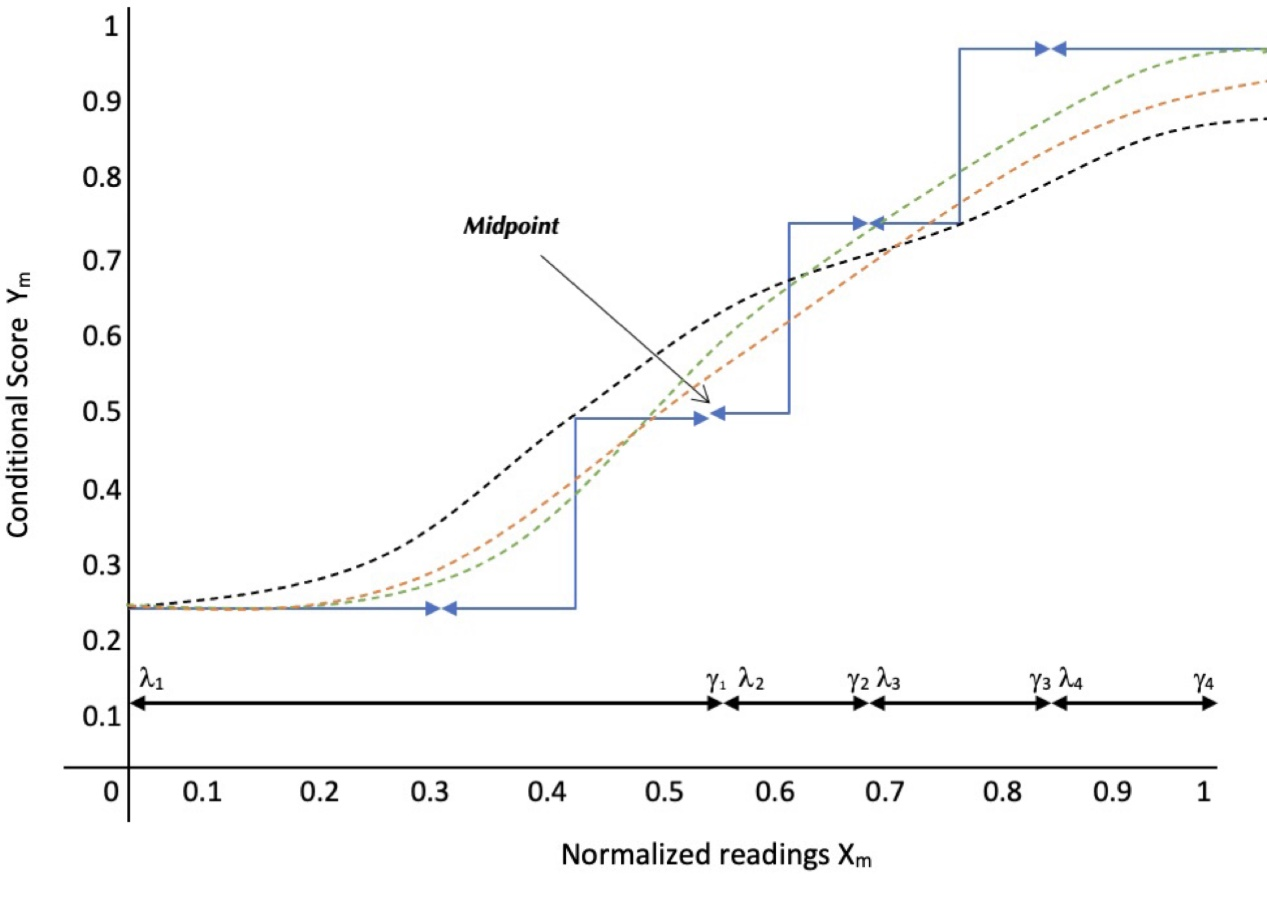
\includegraphics[width=\textwidth]{gfx/Quantizaton_Level.jpg}
    \captionsetup{justification=centering}
    \caption{GRNN interpolation of normalized and conditional.
        \cite{Islam2018CalculatingAH}.}
    \label{fig:Quant}
\end{figure}


The upper and lower limit can be represented in Figure \ref{fig:Quant} in $\lambda$ represents the lower limit and $\gamma$ represents the upper limit of four
conditional ranges.


Representation of four conditional ranges with upper and lower limits are as follows:
\begin{center}
    $Limit Values =
        \begin{bmatrix}
            \lambda_1,D & \lambda_1,D \\
            \lambda_2,D & \lambda_2,D \\
            \lambda_3,D & \lambda_3,D \\
            \lambda_4,D & \lambda_4,D \\
        \end{bmatrix}$
\end{center}

where, $\lambda_i,D = \lambda_i+1,D$ for next ranges and so on. while the targeted midpoint for each quantization
region can be written as
\begin{equation}\label{Equation:4.4}
    \theta_m,D = \frac{\lambda_m,D + \gamma_m,D}{2},
\end{equation}
where $m$ is the quantization levels.

In this approach GRNN is stated as a step function. Due to interpolation technique small changes in measurement of
standard deviation $\Sigma$ does not effect much on the condition score near the boundaries which results in identical
score.

\subsubsection{Feature extraction for HI calculation}
The training set used for GRNN model is the $X_n=R^D$. To get $X_n$ values the mid points of four conditional limits
the conditional score  values(0.25, 0.50, 0.75 and1.0) are represent as Good, Fair, Poor and Very poor. To calculate
the HI score $Y_n$ for each combination of training set $X_n$, the average of each corresponding scores was taken. For
example, if two tests conducted on the subsystem and the test scores are the midpoint of Fair and Very poor, then the
HI score $Y_n$ will be the average of 0.75 and 0.25 which is 0.50. These, $X_n$ and $Y_n$ values are used to train the
GRNN model.

To smoothen the GRNN model, the holdout method is used to calculate the covariance $\Sigma$ stated in
equation \ref{Equation:4.4} for Gaussian Kernel. In holdout approach, one sample from every training set is removed simultaneously and
network is constructed using remaining samples. The network is used to estimate the HI score of a missing sample at a
small values of $E$. Where, $E$ is a multiplicative factor used to provide an appropriate amount of smoothing. The
holdout process is repeated for all sample and the mean- squared error is estimated and stored.

Then, the value of
multiplicative factors is increased in a straight line to 1 with a small incremental step and the whole process is
repeated. Then the mean square for all values of $E$ is plotted. These values used as a multiplicative factor for
$\Sigma_s$, where $\Sigma_s$ is covariance of $X_n$. The process ensure the optimal smoothing to GRNN interpolation for
each subsystem of training set $X_n$. Finally, using equation \ref{Equation_1} the HI score is calculated.


\subsection{Artificial Neural Networks (ANN)}
\vspace*{-12.5mm}\hfill{\fontfamily{phv}\normalsize\emph{Gourav Prakash}}
\label{sec:hi_estimation:approaches:hi_based_rul}

The use of data-driven approaches has gained more popularity due to its non-requirement of prior knowledge of physical
and analytical models with measured data, to predict the future degradation behavior of a system. Data-driven approaches
rely on historically collected data to derive models directly from the data for Remaining Useful Lifetime (RUL) prediction.
Based on this data-driven techniques the RUL can be predicted using HI. In HI-based RUL prediction the model for input
signals against HI is build first and then mapped to estimated HI for RUL.

\subsubsection{HI degradation}

HI estimates the the system health. The heath index is mapped on a graph in respect to time as a degradation line. This
degradation graph represent the the system health index over certain time period. The degradation of HI can be linear or
non-linear. Linear and non-linear graph degradation of HI Figure \ref{fig:HI_Degradation}.

\begin{figure}[ht]
    \centering
    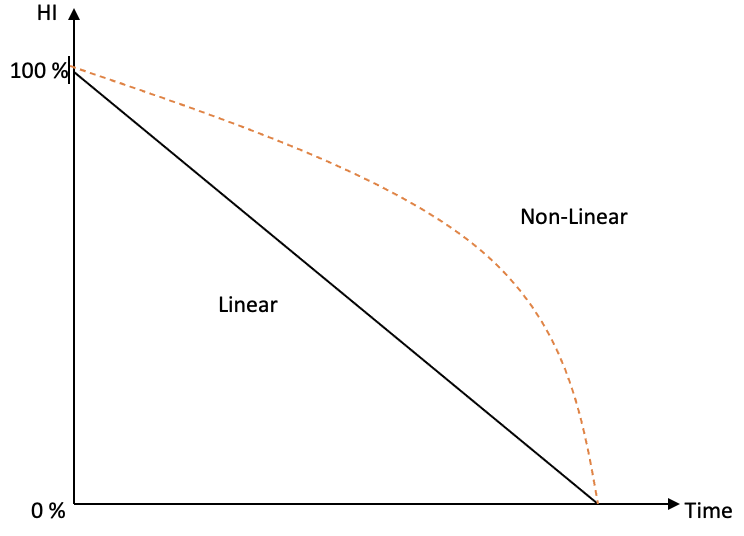
\includegraphics[width=\textwidth]{gfx/HI_Degradation}
    \captionsetup{justification=centering}
    \caption{Linear and non-linear degradation of HI}
    \label{fig:HI_Degradation}
\end{figure}


HI degradation can be linear or non-linear. Linear HI degradation is best known for its simplicity and its easy to
implement. While, non-linear HI degradation is complicated and requires prior knowledge of the system degradation pattern.

\paragraph{Modeling algorithm:}
HI-based RUL prediction is determined by the modeling algorithm. These
modeling algorithm has two stages. First stage is used to learn and predict the HI from instance and second stage is
used to get the RUL from HI. There are many existing modeling algorithm but this paper includes the linear and non-linear
regression model.

Both linear and non-linear models describes the relationship of HI to the time $t$. In case, where HI is shows as non-linear
degradation, a relationship function $f(.)$ is then build by learning algorithm (Neural Network) which makes
\cite{DBLP:journals/tie/YangHZXLN16}
\begin{equation}
    nonlinear[HI]=f(x).
\end{equation}
Similarly, for linear HI a mapping function $g(.)$ is used. By which its assumed that $linear[HI] = g(nonlinear[HI])$, because
Both linear and non-linear model have same ranges between 0,1 and its shows the HI degradation over time $t$. Therefore,
\begin{equation}
    linear[HI] = g(nonlinear[HI]) = g(f(x)) = h(x)
\end{equation}
where, h(.) is the learning algorithm.

\subsubsection{Data Normalization}
Based on the linear degradation HI, data from each of the training motors are used to build multiple independent Neural network
models for predicting HI's. After dynamic smoothing process the HI's are then mapped to the predicted RUL's upon which the
predicted RUL's are assembled to get the final RUL prediction.

During the HI prediction, each testing instance is then normalized based on the parameters calculated from the training instances.
z-score approach
\begin{equation}
    z=\frac{x-\mu}{\sigma}
\end{equation}

where, $\mu$ and $\sigma$ are the mean and standard deviation of a feature in the training data, $x$ is original data, and $z$ is
the normalized data of the features.

\subsection{Ensemble technique}
\vspace*{-12.5mm}\hfill{\fontfamily{phv}\normalsize\emph{Gourav Prakash}}
\label{sec:hi_estimation:approaches:ensemble_technique}

There are several prognostic approaches that are being used to predict the RUL for complex system. One of those prognostic approaches
Ensemble technique is most popular and reliable because of its increase in accuracy and robust behavior. The ensemble predictive
model uses the different ML algorithms or models that are developed using the almost identical datasets which results gives a better
performance compared to single modeling techniques.

The prognostic methods rather than physical and hybrid based it can also be defined as data-driven approach. In data-driven approach
we take the historically collected data and derive the models directly from those data fro the RUL prediction, instead of failure
mechanisms. Data-driven  techniques, the approaches are divided into into categories. FIrst, Direct RUL estimation that models the
relationship between input signals and RUL. Second, HI-based prediction, that uses HI as the training target then map the HI on the RUL.

In this approach we are going to see the HI based techniques to predict the RUL using Ensemble methods. Ensemble methods construct a set
of hypotheses and combine them together. This strengthen the learning algorithm and increase the accuracy of the prediction.

\subsubsection{Methodology}

To develop a predictive model for HI prediction, the raw data were used to extract the valuable information for training purpose regardless of
faulty propagation. To develop a predictive model, the ML algorithm learns the relationship between the training data and the target HI.For the testing phase, testing dataset are provided as input to the predictive model. Thus, the predictive HI is mapped to RUL as
illustrated in Figure \ref{fig:mipet}.

\begin{figure}[ht]
    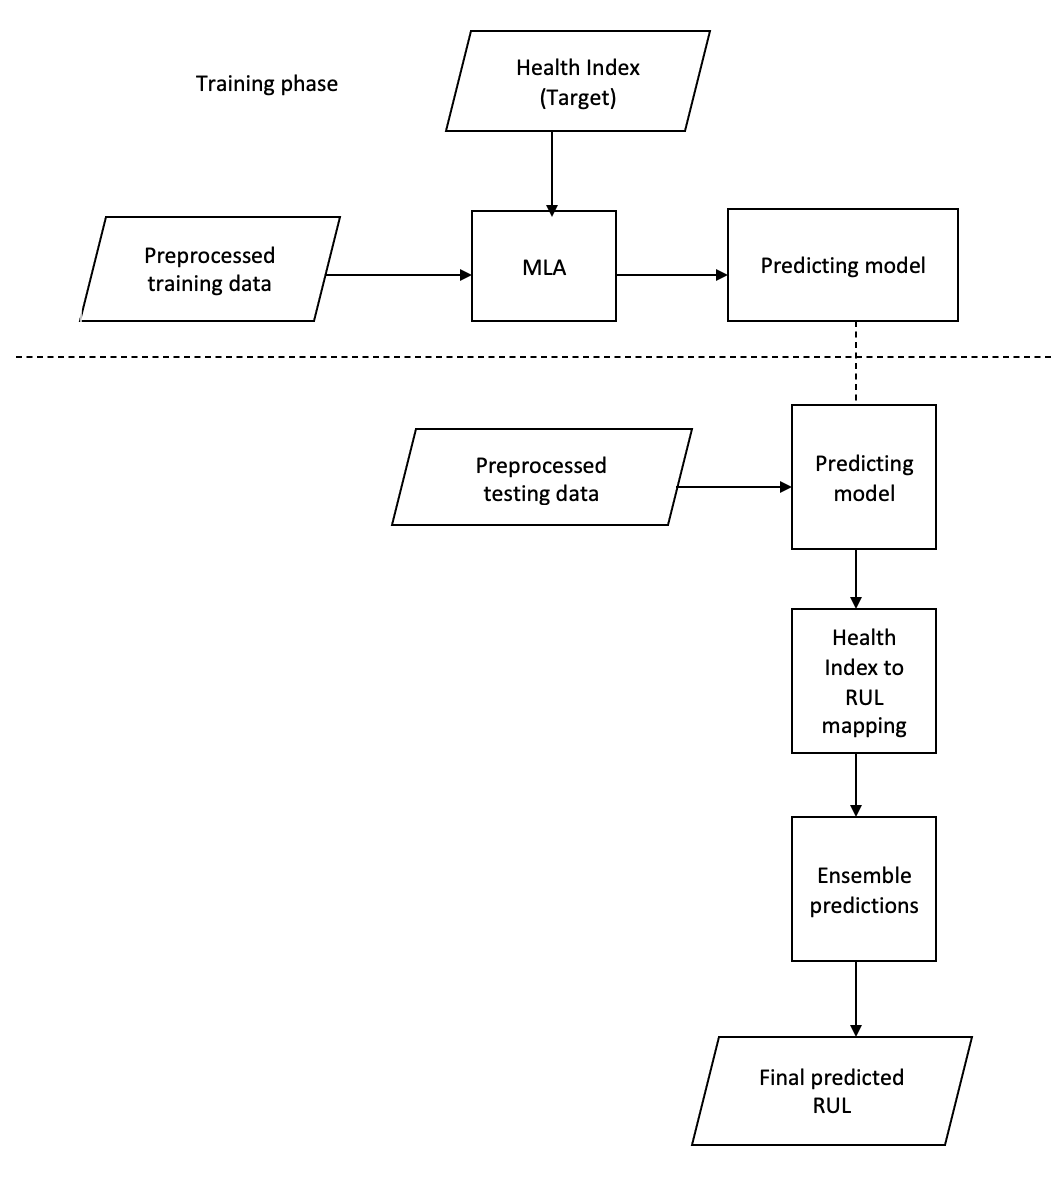
\includegraphics[width=\textwidth,]{gfx/mipet.png}
    \captionsetup{justification=centering}
    \caption{Methodology implementation phases
        \cite{Mutunga2019HealthIndexBP}.}
    \label{fig:mipet}
\end{figure}

\subsubsection{Data processing}
The data type used for this approach is the multi-variant time series data. Each training sample or unit was run to its failure at certain
time. The sensor collects the different measurements related to the system state at runtime.

\begin{figure}[ht]
    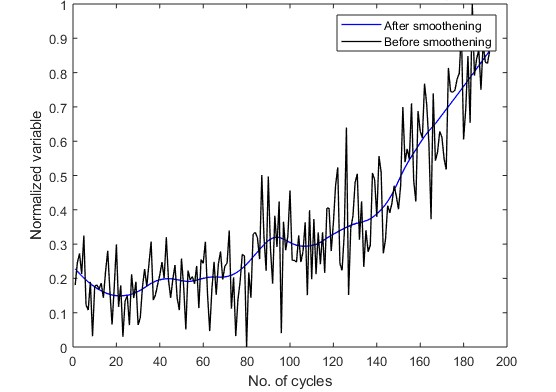
\includegraphics[width=\textwidth]{gfx/Nrmd.png}
    \captionsetup{justification=centering}
    \caption{Data smoothing effects.
        \cite{Mutunga2019HealthIndexBP}.}
    \label{fig:Nrmd}
\end{figure}

In order to identify a smaller subset from the main feature set, a feature selection process was carried out. To reduce the low monotonic values
a monotonicity function $M$ is used,
\begin{equation}
    M=\frac{no.of \frac{dx}{dt}>0-no.of\frac{dx}{dt}<0}{n-1}
\end{equation}

where,
$n$ is the number of observations in a feature, and $dx/dt$ is the derivative of the feature variables with respect to the cycles
\cite{Mutunga2019HealthIndexBP}. THe value of the $M$ ranges between 0 and 1 where, 1 represent the higher monotonic features and 0 represents
non-monotonic features. Therefore, the time variable together with sensors were used as a training datasets. Figure \ref{fig:Nrmd} shows effect of
data smoothing process to remove noises from the data thats allows the important pattern to be revealed. During data modeling, the normalization
$z$-score treats the outliers well, increasing their consistency, and making mapping inputs to the target more efficient.

\begin{equation}
    z=\frac{x-\mu}{\sigma}
\end{equation}

where,

$x$ is the dataset before normalization, $\mu$ and $\sigma$ are the mean and standard deviation for the corresponding variable respectively, and
$z$ is the normalized dataset.

\subsubsection{Auto-Regressive modeling}

Auto-Regression modeling(AR) map the predicted HI to the RUL.To predict the HI values to obtain the degradation trend a sequential representation
of model is illustrated by
\begin{equation}
    HI=\Sigma_{k=1}^m a_k x_{i-k}+e, i=1,2,3,...,n
\end{equation}
where, $a_k$ are the model parameters, $m$ is the model orders, $e_i$ is the model residual and $n$ no.of data points in HI.

\begin{figure}[ht]
    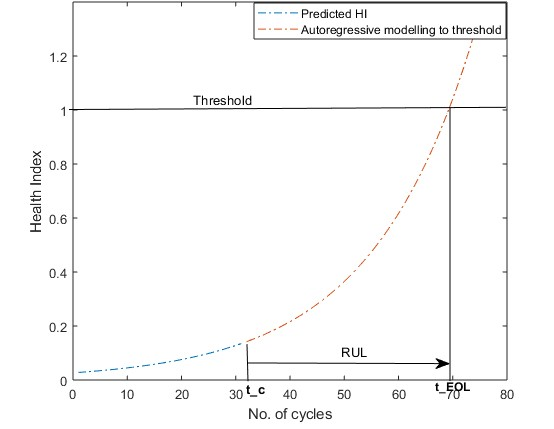
\includegraphics[width=\textwidth]{gfx/Autorm.png}
    \captionsetup{justification=centering}
    \caption{Auto-regression modeling.
        \cite{Mutunga2019HealthIndexBP}.}
    \label{fig:Autorm}
\end{figure}

Figure \ref{fig:Autorm} represents the predicted HI, which has the second section being the corresponding extrapolation to the set threshold of value 1
\cite{Mutunga2019HealthIndexBP}. Where, RUL is defined as the different in number of cycles between current time $t_c$ and the time at end of life
of the system $t_{EOL}$

\subsubsection{Ensemble Techniques}

In ensemble, for different ML algorithm similar datasets with various wearing condition is implemented first. For training datasets, the every similar
number of units the similar amount of predictive models are developed using ML algorithm. During the testing phase, test data for each unit are used as
input to each of the developed models and to the ensembled output. Then, the average are used to obtain the final RUL prediction. Based on the different
ML algorithm used as weighted averaging to aggregate the outputs \cite{Mutunga2019HealthIndexBP},
\begin{equation}
    RUL=\frac{\Sigma_{i=1}^n w_i RUL_i}{\Sigma_{i-1}^n w_i}
\end{equation}

where, $RUL_i$ is the RUL estimated by method $i,w_i$(assigned weight to method $i$ and $n$)which is the number of ML algorithm. For performance evaluation
the prognostics metrics which are selected for performance evaluation of the develop model were Mean Absolute Error($MAE$) , Mean Squared Error($MSE$) and
the Score function as stated in \cite{Mutunga2019HealthIndexBP}.

% For $MAE$ the error is defined as the different between the actual time to failure($AT$) and Estimated time to failure($ET$). So, Error according to $MAE$ is
% \begin{equation}
%     E=AT-ET
% \end{equation}

% Absolute error will be,
% \begin{equation}
%     |E|=|AT-ET|
% \end{equation}

The $MAE$ can be calculated as the average of the absolute error$E$ for each $n$ number of units.

% \begin{equation}
%     MAE=\frac{1}{n}\Sigma_{i=1}^n |E|
% \end{equation}

% Based on the $MAE$ the Mean Square Error $MSE$ is calculated as,
% \begin{equation}
%     MSE=\frac{1}{n}\Sigma_{i=1}^n E^2
% \end{equation}

The score function is the weighted sum of RUL errors and estimated metric score.

\begin{equation}
    S=s_1+s_2
\end{equation}

\begin{equation}
    s_1(E<0)=\Sigma_{i=1}^n e^{-\frac{E}{a_1}}
\end{equation}

\begin{equation}
    s_2(E\geq0)=\Sigma_{i=1}^n e^{\frac{E}{a_2}}
\end{equation}

where,
$S$ is the computed score, $n$ is the number of prediction units, and $E$ is the error terms.


\subsection{LSTM Encoder-Decoder}
\vspace*{-12.5mm}\hfill{\fontfamily{phv}\normalsize\emph{Selami Hoxha}}
\label{sec:hi_estimation:approaches:lstmencoder}

In the paper by Malhotra et al.,\cite{DBLP:journals/corr/MalhotraTRAVAS16}, an approach for estimating HI based on encoder-decoder
with hidden units being Long Short Term Memory (LSTM) units is presented and is called LSTM-ED (Long Short-Term Memory - Encoder Decoder).
A traditional way of calculating RUL for a system is to build a HI based on assumption that it follows a linear or exponential degradation
curve, where this curve is later extrapolated to a RUL. The problem with this approach is that the degradation of a system will not always follow
such a curve. LSTM-ED does not assume the shape of degradation curve. LSTM-ED will learn an
encoder-decoder model, then the model will learn an encoding of a sequence into some shorter representation and at the same time learns
to decode that encoded sequence into the original sequence. When this model is used for reconstructing to the original sequence, it will generate
some error which is called reconstruction error and is the basis of how the HI curve will be calculated.


\paragraph{Principal Component Analysis}
Principal Component Analysis (PCA) is an important tool which will be
used in a few approaches in this chapter, starting with LSTM-ED.
PCA is a dimensionality reduction algorithm. The dimensionality is reduced by projecting the data into a lower linear subspace
that minimizes the reconstruction error. Given the data matrix $X$, with N dimensions, where each element is centered to the mean of
the data, the PCA algorithm tries to find the optimal orthogonal projection matrix $P^{*}$ to the $k^{th}$ dimension by minimizing:
\begin{equation}
    P^{*} = \min_{P \in P_k} ||PX-X||_F^2
\end{equation}
where $P_k$ is the set of matrices that are N-dimensional and have a rank of $k$.
This way the dimensionality of X is reduced from N to k where $N>k$ without losing too much information
about the data. Another interpretation is that the dimensions with the biggest variance are kept. These k
dimensions that retain the most information about the data are called the principal components. \cite{MohriFML}

\paragraph{LSTM unit}
A LSTM unit or cell, is a neural network cell which is capable to process sequential data. It is structured in such a way that is able to
save important information about the input and forget the information that is not useful. The LSTM cell is made of several gates as shown
in figure \ref{fig:lstm_unit}. The gates process the data using the equations:
\begin{equation}
    \begin{aligned}
        i_t = \sigma(W_i h_{t-1} + W_i h_t)                          \\
        f_t = \sigma(W_f h_{t-1} + W_f h_t)                          \\
        o_t = \sigma(W_o h_{t-1} + W_o h_t)                          \\
        \tilde{c} = \tanh(W_{\tilde{c}} h_{t-1} + W_{\tilde{c}} h_t) \\
    \end{aligned}
\end{equation}

where $x_t$ is the input vector, $h_t$ is the output vector, $i_t$ is the input gate, $f_t$ is the
forget gate, $o_t$ is the output gate, $\tilde{c}$ is the intermediate memory cell, and W are the model
parameters.
Then the cell memory and the output vector are calculated and are both output to be processed
by the next cell. The cell memory and output vector are calculated by the following:
\begin{equation}
    \begin{aligned}
        c_t = (i_t  \tilde{c}_t) + (f_t c_{t-1}) \\
        h_t = o_t \tanh(c_t)
    \end{aligned}
\end{equation}
here $c_t$ is the cell state.
\cite{LSTMandGRU}

\begin{figure}[ht]
    \centering
    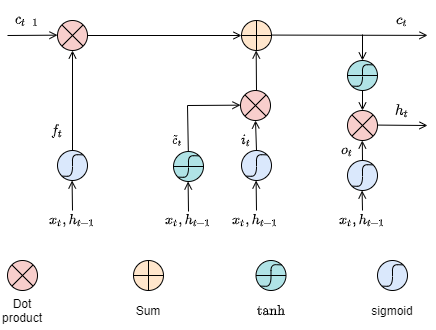
\includegraphics[scale=0.7]{gfx/LSTM_unit}
    \captionsetup{justification=centering}
    \caption{LSTM unit structure \cite{LSTMandGRU}}
    \label{fig:lstm_unit}
\end{figure}

\paragraph{HI construction}
Let us denote with $X^{(i)} = [x_i^{(1)} ,  x_i^{(2)} , \dots , x_{i}^{(\tau(i))}]$ with $x_i^{(t)} \in \mathbb{R}^{|S|}$ defined as in section
\ref{sec:intro:time-series-definition}
and $\tau(i) = \tau(i,s)$ for all $s \in S$ denotes the number of time steps until the end of life (the failure occurs) of
a system, which in this case is the assumed
to be the same for all the sensors. Next, the sensor data of each time step is z-normalized.
Let $\mu_j$ and $\sigma_j$ be the mean and standard deviation calculated sensor wise with j denoting the sensor. The
elements in  $X^{(i)}$ will take the form $\frac{x^{(t)}_{ij}-\mu_j}{\sigma_j}$, where $x^{(t)}_{ij}$ is the reading of $j^{th}$ sensor
of instance $i$ at time step $t$. Since in real world the sensor data is correlated, a
dimensionality reduction algorithm is applied. In our case PCA is applied to achieve what is called "the derived data" on
which the next steps will be taken. The derived data is denoted as $Z^{(i)} = [z_i^{(1)}, \,  z_i^{(2)}, \, \dots \, ,z_{i}^{(\tau(i))}]$ where
$z_i^{(t)} \in \mathbb{R}^p$, with $p$ being the number of principal components.

To train a LSTM ED network, subsequences of length \emph{l} from all the training instances are used. More precisely the first \emph{l} elements which
are assumed to represent a healthy state of the system are used for training.
First, the encoder is trained, given the time series
$Z = [z_1, \,  z_2, \, \dots ,z_l]$, $a_t^{(E)}$, the hidden state of the encoder at time $t$ for each $t \in \{1,2,\dots,l\}$, where
$a_t^{(E)}\in R^c$, with $c$ being the number of LSTM units in the hidden layer of the encoder. The decoder is trained jointly with
the encoder. The decoder is initialized in the reverse order, hence the reconstructed time series is output in the reverse order $Z = [z_l, \,  z_{l-1}, \, \dots ,z_1]$. The process is shown in figure \ref{fig:LSTM_inference}.

\begin{figure}[ht]
    \centering
    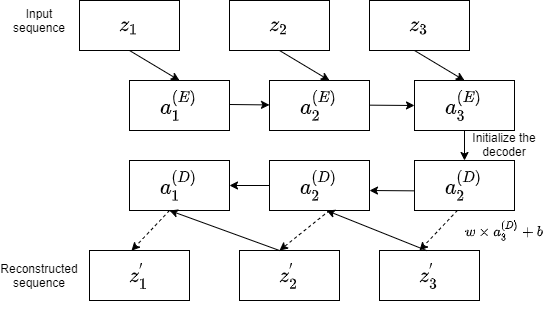
\includegraphics[scale=0.6]{gfx/LSTM_ED_inference}
    \captionsetup{justification=centering}
    \caption{LSTM-ED neural network structure
        \cite{DBLP:journals/corr/MalhotraTRAVAS16}}
    \label{fig:LSTM_inference}
\end{figure}

To reconstruct all the possible subsequences, a sliding window of size \emph{l} is used.
This means that there will
be $L-l+1$ subsequences of length \emph{l}. Also, it is important to note that an element $z_t$ will be calculated at most \emph{l} times,
or every time it is part of some subsequence. To get the final values an averaging is performed. Finally, the
reconstruction error for time step t is given $e_t^{(i)} = ||z_t^{(i)} - z_t^{'(i)}||$, where $z^{'}$ is the reconstructed sequence.
The model's optimization goal is to minimize
$E = \sum_{i\in[N]}\sum_{t=1}^{l}{{\left( e_t^{(i)} \right)}^2}$.

After the reconstruction error is calculated, it is scaled to obtain the target HI $h_t^{(i)}$ as:
\begin{equation}
    h_t^{(i)} = \frac{e_M^{(i)}-e_t^{(i)}}{e_M^{(i)}-e_m^{(i)}}
\end{equation} where $e_M^{(i)}$ and $e_m^{(i)}$ are the maximum and the minimum value of the reconstruction error respectively.

From the target HI calculated for each time-step $t$, we obtain a sequence of these HI which we call
the degradation curve. We note it by $H = [h^1_{(i)}, \, h^2_{(i)}, \, \dots ,\, h^{\tau(i)}_{(i)}]$.
For calculating RUL of the some new instance $i^*$, at first we need to build its degradation curve. The degradation curve is calculated
by first training a linear regression model for the time series data, where the target is the constructed HI. The Linear
regression has the form:

\begin{equation}
    f_{\theta}(z_t^{(i)})  = \theta^T z_t^{(i)} + \theta_0
\end{equation} where $\theta \in \mathbb{R}^p$, $\theta_0 \in \mathbb{R}$.



\subsection{Hierarchical Gated Recurrent Unit Network}
\vspace*{-12.5mm}\hfill{\fontfamily{phv}\normalsize\emph{Selami Hoxha}}
\label{sec:hi_estimation:approaches:HGRUN}

Gated Recurrent Unit Network (GRUN) is a Recurrent Neural Network (RNN) that has been successfully applied in health prognosis. In the paper
by Li et al., \cite{LI2019229},
the GRUN approach is used to determine HI degradation based on bearing historical data, which is used to determine future HI and
calculate RUL of the bearings. The approach presented in the paper is described in detail in the following.\\

\paragraph{Gated Recurrent Unit}
A gated recurrent unit is a variant of LSTM unit with a simplified architecture. It is made of an update gate which determines how
the hidden state $h_t$ will be modified by the candidate state $c_t$, and a reset gate which determines which part of the previous hidden
state $h_{t-1}$ to be ignored. The weights of GRU unit are calculated with a forward pass as follows:
\begin{equation}
    \begin{aligned}
        z_t = \sigma(W_{xz}x_t+U_{hz}h_{t-1}+b_z)             \\
        r_t = \tanh(W_{xr}x_t+U_{hr}h_{t-1}+b_r)              \\
        c_t = \tanh(W_{xc}x_t +U_{hc}(r_t \odot h_{t-1})+b_c) \\
        h_t = (1-z_t) \odot h_{t-1} + z_t \odot c_t
    \end{aligned}
\end{equation}
where $x_t$ is the input; $\sigma$ and $\tanh$ are the activation functions; $c_t$ is the candidate state; $h_t$ is the output of a unit;
$W_{xz}$, $W_{xr}$, and $W_{xc}$ are the weight matrices between the layers as noted in their subscript; $U_{hz}$, $U_{hr}$, and $U_{hc}$
are the weights of the cycles; $b_z$ $b_r$, and $b_h$ are the biases.

\begin{figure}[ht]
    \centering
    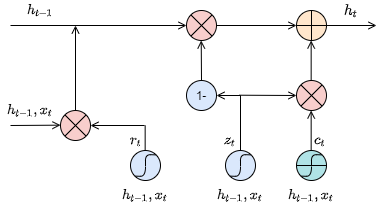
\includegraphics[scale=0.7]{gfx/GRU_unit}
    \captionsetup{justification=centering}
    \caption{GRU structure \cite{LSTMandGRU}}
    \label{fig:GRU_unit}
\end{figure}

\paragraph{The HI construction}

The HI is designed in several steps, starting with feature extraction, then applying a kernel principal component analysis (KPCA) to
extract the features that contain the most information about the data, followed by a smoothing via exponentially weighted moving
average (EWMA). The designed HIs are then used to learn a model using Hierarchical Gated Recurrent Unit Network (HGRUN)
which will be used to estimate HI for new instances of
time series data.
The first step in learning a model for the given time series data is to extract a set of features.
The process of feature extraction is given in detail in sections \ref{sec:feature-extraction:approaches:time-domain},
\ref{sec:feature-extraction:approaches:frequency-domain} and \ref{sec:feature-extraction:approaches:time-frequency-domain}.
The set of features is made of time domain, frequency domain and time-frequency domain features extracted from the time series data.
The features extracted from the time domain are Root mean square (RMS), absolute mean value (AE), square
root amplitude (SRA), variance and peak-to-peak value. From the frequency domain spectrum RMS, spectrum mean value and spectrum shape
factor are the extracted features. From time-frequency domain maximum value, RMS and SRA of the second-frequency-band signals, which are extracted
by the three-layer wavelet packet transformation. Only a handful of these high dimensional features will contain useful data. Therefore
the next step is to apply KPCA to extract the useful features. The KPCA performs PCA on data transformed to a higher dimensional feature space using
a kernel and then PCA is applied on the transformed data \cite{MohriFML}. The first step is to
map the data to a high dimensional space using the kernel and then applying the PCA algorithm to extract the actual principal components.
The first principal component $ p = [p_1,p_2,\dots,p_t]$ will be the HI, and will represent the bearing degradation. Since the HI
usually contains fluctuations, EMWA smoothing is applied. EMWA modifies the HI by approximating it with the value
\begin{equation}
    f_t = \alpha(p_t + \beta p_{t-1}+\beta^2p_{t-2}+\dots+\beta^{t-1}p_1).
\end{equation}
where $0< \alpha <1$ is called the smoothing parameter and $\beta$ is equal to $1-\alpha$. The value
$f_t$ is the HI after smoothing is applied and $p_t$ is the actual HI. The smoothed value is determined
by considering all the HI in the degradation curve, with the actual value $p_t$ having the biggest
influence and the other HI have exponentially decaying influence the farther they are in the degradation
curve.

\paragraph{The HGRUN model}

Since the rolling bearing degradation is is made of time-series parameters and since degradation is often nonlinear, a powerful
nonlinear model is required. To achieve such a powerful model, HGRUN is built with multiple GRU layers and with a regression layer
on top of the last GRU layer, as shown in fig \ref{fig:HGRUN_model}.

\begin{figure}[ht]
    \centering
    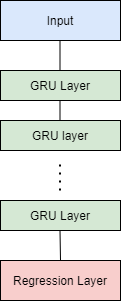
\includegraphics[scale=0.7]{gfx/HGRUN_model}
    \captionsetup{justification=centering}
    \caption{HGRUN structure}
    \label{fig:HGRUN_model}
\end{figure}

Since HGRUN is a RNN model, it is trained using back propagation through time and gradient descent.
The goal of the model is to minimize MSE.
\begin{equation}
    MSE = \frac{1}{2T}\sum_{t=1}^N (y_t-\hat{y}_t)^2
\end{equation}
where $y_t$ is the predicted value and $\hat{y}_t$ is the actual label. In the work presented AdaGrad
(Adaptive Gradient Descent) was used for fast convergence.
The AdaGrad algorithm is a modification of gradient descent and its parameters are updated
adaptively as follows:
\begin{equation}
    \begin{aligned}
        \eta_e = \frac{\eta_0}{\sqrt{\sum_{i=1}^e g_i^2 +\epsilon}} \\
        \upsilon_e = \mu \cdot \upsilon_{e-1} - \eta_e \cdot g_e    \\
        \theta_e = \theta_{e-1} + \upsilon_e
    \end{aligned}
\end{equation}
where $e$ is the epoch number; $\eta_e$ is the learning of the e-th epoch; $\epsilon$ is a value that ensures that the denominator
is never zero; $g_e$ is the e-th gradient; $\mu$ is the momentum; $\theta_e$ are the parameters at the e-th epoch and $v_e$ is the
e-th updating value.


\paragraph{Estimating the HI}

To predict future HI values a HGRUN model is also trained. The model is trained using training and testing samples which are designed
using the HI as calculated above. Suppose we have $N$ data points $(f_1, f_2, ... , f_N)$ calculated using the HI design explained
above for each time series raw samples. Using these N data points and the one-step look ahead technique, the samples for training and
testing HGRUN model are created. The first training example $e_1$ is formed by taking $(f_1, f_2, ..., f_{\emph{l}})$ as the sample
and $f_{\emph{l}+1}$ as the label. For the second example, the sample would be $(f_1, f_2, ..., f_{\emph{l}+1})$ and the label
$f_{\emph{l}+2}$. The training samples are formed until some point $k$, which means there are $N-l-k$ training samples. And then the
other data points $(f_k, ... , f_N)$ are used to create similarly the testing samples.

\subsection{Kullback Leibler Divergence}
\vspace*{-12.5mm}\hfill{\fontfamily{phv}\normalsize\emph{Selami Hoxha}}
\label{sec:hi_estimation:approaches:kullbackLeibler}

In the paper by Aremu et al.,\cite{DBLP:conf/indin/AremuOHM19} an approach based on information entropy is presented that captures the degradation of
multi sensor systems. PdM systems that perform condition monitoring based on raw data perform poorly according to the author.
An appropriate measure for the health condition of a system is needed to capture the degradation of the system accurately.
The multi sensor systems also pose a challenge for capturing the degradation of the system, since not all sensors have influence
on capturing the degradation of the system.  This is a model-free approach and is based on information entropy measure known as
Kullback-Leibler Divergence (KLD). As in LSTM-ED, it is assumed that the first \emph{l} time steps in the series
data represent a healthy state of a system. Then a tool that makes it possible to compare this representation
of the healthy system to other instances is used to build the HI.\\

The healthy state of the system in this work is represented by its distribution of the data. And in order
to compare the distribution of the entire
life of a system to the healthy data distribution the concept of entropy needs to be introduced. In
\cite{DBLP:conf/indin/AremuOHM19}, entropy is defined as:
'Entropy or information entropy is the measure of "unexpectedness" of data in a variable, obtained by quantifying its contained
uncertainty'. The entropy can be measured using the Shanon entropy, which is given by the formula:
\begin{equation}
    H(X) = - \sum_{x \in X} p(x) \log p(x)
\end{equation}
where $X$ is a random variable. The sum is over all the possible outcomes $x$ of the variable $X$ and
$p(x)$ is the probability of the distribution.
An important concept that is needed next is to be able to capture how much the distribution will change when some other event happens.
This change is measured by KLD. \newline Given the distributions $P$ and $Q$, KLD is given as follows:
\begin{equation}
    H(P||Q) := \sum_{x \in X} p(x) \log \frac{p(x)}{q(x)}
\end{equation}
with $H(P||P)=0$ and $H(P||Q) \neq H(Q||P)$ \\



Given the time series data $ X \in \mathbb{R}^{N \times u}$ where $N$ is the number of samples,
$u=|S|$ is the number of sensors and as before by $i$ we denote the $i^{th}$ instance of time series,
several steps are taken for the HI to be constructed. First, each sensor data
is used to parametrize a logistic distribution based on the first \emph{l} observations.

\begin{equation}
    X_i \sim \text{logistic}(\lambda_i, \sigma_i).
\end{equation}

The logistic distribution shape is determined by its parameters, with $\lambda$ being the location parameter that determines where the distribution will
be centered and $\sigma$ will determine how focused is the distribution around the center. A depiction of logistic distribution on two sets of parameters is
shown in figure \ref{fig:logistic_dist}.
Then, the probability density of each sensor data that represent a healthy system can be calculated by:
\begin{equation}
    f_i^s(x_i^s; \lambda_i^s, \sigma_i^s) = \frac{1}{\sigma_i^s}
    exp \bigg(-\frac{x_i^s - \lambda_i^s}{\sigma_i^s}\bigg){\bigg(1+exp \bigg(-\frac{x_i^s - \lambda_i^s}{\sigma_i^s}\bigg)\bigg)^{-2}}
\end{equation}

where we see that also the probability density function (pdf) is parametrized and $1<s<u$.

\begin{figure}[ht]
    \centering
    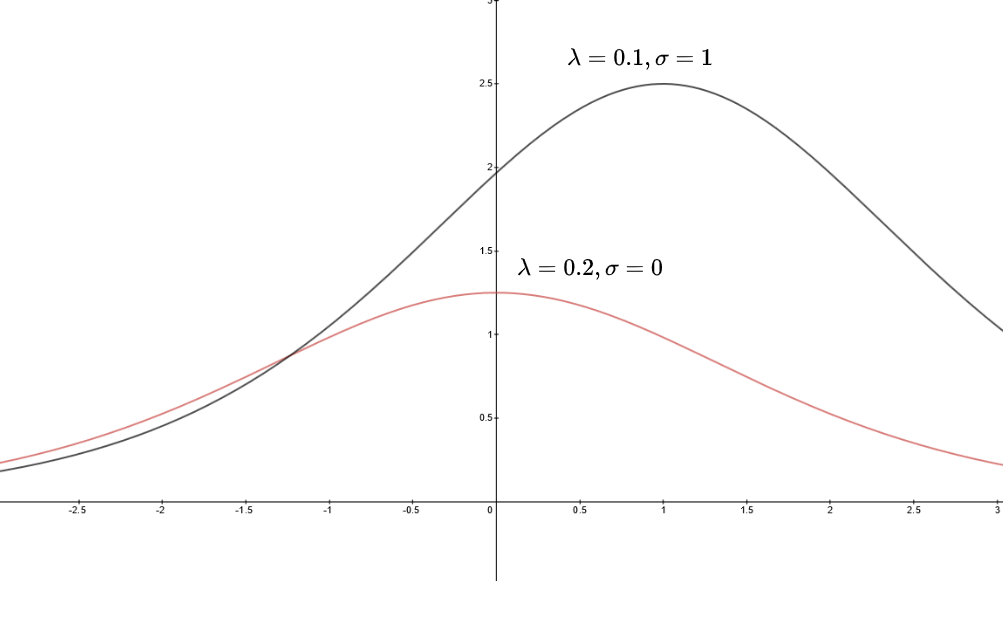
\includegraphics[scale =0.25]{gfx/logistic_dist}
    \captionsetup{justification=centering}
    \caption{Logistic distribution on two different sets of parameters}
    \label{fig:logistic_dist}
\end{figure}


Let $P^s$ be the distribution of observations in the healthy state of the system and $\zeta_k^s$ ($k=1,2,\dots, N$)
be the same distribution modified after seeing an observation from sensor s. The HI is defined as the KLD between the distributions $P^s$ and $\zeta_k^s$:
\begin{equation}
    H(P^s||\zeta_k^s) := \sum_{j=1}^{\emph{l}} \rho^s_j \log \frac{\rho_j}{\zeta_{kj}^s}
\end{equation}
where $1<k<N$.
\begin{equation}
    \rho_j^s = f_i^s(x_{i_j}^s; \lambda_i^s, \sigma_i^s)
\end{equation}
and
\begin{equation}
    \zeta_{kj} = f_i^s(y_j^s; \lambda_i^s=x_k^s, \sigma_i^s)
\end{equation}
where $y_j$ is generated by a random variable $Y^s$. $Y^s$ is a random variable generated by $X_n^s$ supported logistic regression with
the location parameter being the sample $x_k^s$. That means
\begin{equation}
    Y^s \sim \text{logistic}_{X_i^s}(\lambda_i = x_k^s, \sigma_i)
\end{equation}

Then the HI for a single sensor is given by:

\begin{equation}
    \hat{\emph{f}}_H^{\,\,s} = \{H(P^q||\zeta_1^s),H(P^q||\zeta_2^s),\dots ,H(P^s||\zeta_N^s)\}
\end{equation}


and finally the HIs of all the sensors are is given by the set:

\begin{equation}
    \label{sec:hi_estimation:kullback_leibler:HI_set}
    X_H = \big\{ \{ \hat{f}_H^{\,\, 1^T} , \hat{f}_H^{\,\, 2^T},\dots, \hat{f}_H^{\,\, u^T} \} \big\}
\end{equation}
.

If $H(P^q||\zeta_k^s) \neq H(P^q||\zeta_{k-1}^s)$ then wear has ocurred in the system.

\textbf{Selecting the sensors}

For performing feature selection, which in this case means selecting the sensors, KLD analysis of system complete lifecycle is evaluated.
This is done for each sensor using the following formula:
\begin{equation}
    \Delta_H^s =
    \left(H(P^q||\zeta_1^s)-H(P^q||\zeta_N^s)\right)
    \left(\frac{H(P^q||\zeta_1^s)+H(P^q||\zeta_N^s)}{2}\right)^{-1}
\end{equation}

If $\Delta_H^s$ is not greater than zero it means that the sensor does not show any degradation trend. Using this fact sensor selection
is performed by excluding the HI for the sensors that do not show any degradation trend. The set
of HI in equation \ref{sec:hi_estimation:kullback_leibler:HI_set} becomes:
\begin{equation}
    X_H = \big\{ \{ \hat{f}_H^{\,\, 1^T} , \hat{f}_H^{\,\, 2^T},\dots, \hat{f}_H^{\,\, u^T} \} | \Delta_H^s>0 \big\}
\end{equation}
.

Finally, the health indicator set can be used to train a supervised model where the target is the actual RUL.
This model can finally be used to estimate the RUL. Random forests and gaussian processes were applied in
the presented paper.

\newpage
\section{Evaluation}
\vspace*{-15mm}
\hfill{\fontfamily{phv}\normalsize\emph{Selami Hoxha}}
\label{sec:hi_estimation:evaluation}

The estimated HI should be a good representation of the actual state of the system for successful prognostics.
The evaluation of the HI is based on a test dataset, as presented in
\ref{sec:hi_estimation:formal_definiton}
which contains the instances of time series, that are not used
in the training process, and have information encoded for that instance. The information could be the actual
HI for every time step in the series, which is usually not the case in publicly available data, or the RUL. If we
have the actual HI for every time step in the test dataset, then using some metric we could compare the estimated value
with the actual value to measure its performance. Since publicly available datasets usually contain RUL, to get
the actual HI the RUL is extrapolated to an HI using some linear or exponential function
\cite{DBLP:journals/corr/MalhotraTRAVAS16} and this HI is compared to the estimated HI. Another way of measuring
the performance of HI is by using the estimated HI to get the RUL and then measure the performance by using some
metric that compares the actual RUL to the estimated one.

Several different metrics are being used in the research \cite{Islam2018CalculatingAH, LI2019229,
    DBLP:journals/tie/YangHZXLN16, Mutunga2019HealthIndexBP, DBLP:journals/corr/MalhotraTRAVAS16}. The metrics vary based on how
they handle late and early predictions.
A late prediction
is when the HI predicts that the system is healthier than it actually is, resulting in the system running into
failure before it can  be repaired. An early prediction is when the HI predicts
the system as lower than its actual value, which would mean that we repair the system that could have been functional for a longer time. The loss functions can be symmetric, where the late predictions and early predictions
are penalized equally, or asymmetric where the loss function has some parameter that decided on how to penalize
wrong predictions.
There are also metrics that operate on the whole degradation curve (represented by a vector of HIs ordered by the time step)\cite{DBLP:conf/indin/AremuOHM19}.

Let us denote by $y$ the actual value of HI or RUL, and by $\hat{y}$ the
estimated HI or RUL. Also, let $C$ denote the degradation curve. Finally, with $M$ is the
number of test instances.

\subsubsection{Symmetric loss functions}

Symmetric loss functions evaluate the estimated HI by penalizing the late predictions equally as early predictions. The smaller the loss, calculated using the loss functions,
the better the performance of the approach. In the following, symmetric loss
functions that are used for evaluating HI performance are presented.

\paragraph{Mean Squared Error}
\begin{equation}
    MSE = \frac{1}{M} \sum_{t=1}^M(y_t - \hat{y}_t)^2
\end{equation}
\cite{Islam2018CalculatingAH}.

\paragraph{Root Mean Squared Error (RMSE)}
\begin{equation}
    RMSE = \sqrt{\frac{1}{M-1} \sum_{t=1}^M(y_t - \hat{y}_t)^2}
\end{equation}
\cite{DBLP:journals/tie/YangHZXLN16}.

\paragraph{Maximum Absolute Error (maxAE)}
\begin{equation}
    maxAE = \max_{1 \leq t \leq M} (|y_t - \hat{y}_t|)
\end{equation}
\cite{LI2019229}.

\paragraph{Normal Mean Squared Error (NMSE)}
\begin{equation}
    NMSE = \frac{\sum_{t=1}^M (y_t - \hat{y}_t)^2}{\sum_{t=1}^M \hat{y}_t^2}
\end{equation}
\cite{LI2019229}.

\subsubsection{Assymetric score functions}

Asymmetric score functions evaluate an approach by penalizing early predictions and late
predictions in different amounts. Score functions are parametrized to achieve the
asymmetric evaluation. The bigger the score calculated by the score function
the better is the performance of the approach being evaluated.

\paragraph{Scoring function}

The scoring function can be used to penalize early predictions or late
predictions by controlling the parameters $\alpha_1$ and
$\alpha_2$.
\begin{equation}
    S=s_1+s_2
\end{equation}
where by denoting $E = y-\hat{y}$ we have, if $E<0$
\begin{equation}
    s_1 = \sum^M_{t=1} \exp{\left(-\frac{E}{\alpha_1}\right)}
\end{equation}
and if $E \geq 0$ then
\begin{equation}
    s_1 = \sum^M_{t=1} \exp{\left(\frac{E}{\alpha_2}\right)}.
\end{equation}
For both early and late predictions the error grows exponentially
\cite{Mutunga2019HealthIndexBP}.



\paragraph{Timeliness score}
Timeliness score is an asymmetric score function that is parametrized with the parameter $\gamma$,
where $\gamma = \frac{1}{a}$ if $\hat{y} - y \leq 0$ else $\gamma = \frac{1}{b} $ if $\hat{y} - y \geq 0$. If $a>b$ then late predictions ($\hat{y} - y \leq 0$) are penalized
more (by being divided with a greater number). Similarly, if $b>a$ then early prediction
will be penalized more.
This is formulated as follows:
\begin{equation}
    E = \sum_{i^* =1}^N (exp(\gamma |\hat{y} - y|)-1)
\end{equation}
Usually a > b is chosen, to
penalize late predictions more than early predictions \cite{DBLP:journals/corr/MalhotraTRAVAS16}.




\subsubsection{Degradation curve based evaluation functions}

A health degradation curve is the representation of the degradation of the health of the system.
The degradation curve is represented by HIs ordered in a sequence by the time step,
$C = [c_1, c_2, \dots ,c_K]$ with K
being the length of the sequence.


\paragraph{Monotonicity}
To evaluate if the HI degradation curve is a good representation of degradation of the system monotonicity measure and robustness measure are used. HI degradation curve should have an
increasing or decreasing degradation trend. Monotonicity is measured using the following metric:
\begin{equation}
    Mon(C) = \frac{1}{K-1}|N_{d/dc>0}-N_{d/dc<0}|
\end{equation}
where C is the HI degradation curve, the length of the HI curve is K and $d/dk=c_{k+1} - c_k$ is the difference between the HI in the sequence. The values range from 0 to 1,
where 1 indicates that the degradation curve is a good representation of the degradation
of the system (has strong monotonicity).
\cite{DBLP:conf/indin/AremuOHM19}.

\paragraph{Robustness}
Robustness measures the robustness of the HI degradation curve to noise. A good HI degradation
curve should be able to give good results in systems that
contain noisy data. The robustness measure is given by:
\begin{equation}
    Rob(C) = \frac{1}{K} \sum_{k=1}^K \exp \left(-\bigg| \frac{c_k-c_k^T}{c_k} \bigg|\right)
\end{equation}
where  $c_k^T$ is the mean value at $k^th$ element. The values range from 0 to 1, where
the value 1 represents a very smooth degradation curve.
\cite{DBLP:conf/indin/AremuOHM19}.               % INCLUDE: health index estimation
% !TEX root = ../main.tex
%
\chapter{Remaining Useful Lifetime Estimation}
\label{sec:rul_estimation}
\vspace*{-15mm}\hfill{\fontfamily{phv}\normalsize\emph{Vinay Kaundinya and Christopher Zinda}}

\cleanchapterquote{Better three hours too soon than a minute too late.}{William Shakespeare}{(Playwrite and poet)}

In this chapter, we present one of the most challenging Predictive Maintenance topics which is estimating the remaining useful lifetime (RUL) of a machine. We describe what RUL estimation is and why it is so important for manufacturers. In section~\ref{sec:rul_estimation:datasets} we provided a list of current datasets that can be used when testing a RUL approach. Section~\ref{sec:rul_estimation:approaches} will then give a deeper insight into six state-of-the-art approaches for predicting the RUL. The chapter closes with a summary of the most common metrics and loss functions that are used in combination with RUL estimation. In summary, this chapter will provide an insight into all important specifics to this PdM topic and the building blocks that are needed to implement RUL estimation.

\section{Motivation}
\vspace*{-12.5mm}\hfill{\fontfamily{phv}\normalsize\emph{Christopher Zinda}}
\label{sec:rul_estimation:motivation}

The 4th industrial revolution is presenting companies with enormous challenges. More and more processes are digitalized and the shopfloor is showing an increasing number of IoT devices. Most manufacturers equip their production lines with sensors that record a number of different properties. This enables them to collect large amounts of data that can be used for advanced Predictive Maintenance approaches.\\
One of the biggest cost factors in production is unscheduled downtime i.e. unexpected machine failure. Unexpected downtime is tied to immediate costs because the products can not be manufactured and will cause a delay for the customer. Also, replacement parts might not be in stock and even cause a greater delay until the production can continue. These unexpected events can occur when the statistical models that were created by experts do not reflect the real behavior. Due to the high complexity of these machines, there are also a lot of known and unknown variables that influence the Useful Lifetime of a machine. Using state-of-the-art approaches for RUL estimation, the risk of an unplanned downtime can be reduced by large amounts. The approaches try to learn the complex dependencies between the different sensors to obtain an approximate model of the machine. The main goal is to predict the time that a machine has left before a failure will occur. This can be achieved using any of the approaches that we describe in section~\ref{sec:rul_estimation:approaches}. With this information being known a priori the maintenance department can schedule a planned maintenance of the machine and ensure that replacement parts are already available. This way the costs can be drastically reduced. These types of machine learning approaches are slowly introduced in practice and there will be a lot of use cases in the future.

\subsection*{Challenges}
\label{sec:rul_estimation:motivation:challenges}

There are multiple challenges that arise when dealing with data driven approaches. Handling real time data from a factory implies a lot of unknown factors. We will describe some of the challenges that arise when trying to estimate RUL.

\subsubsection*{Health degradation trend}

For complex machines, it is very difficult to model their health degradation mathematically \cite{DBLP:journals/corr/abs-1709-01073}. There are many approaches that assume a certain degradation trend e.g. exponential degradation, but this might not relate to the true physical behavior of the machine. Often times there is no indication of the current health state, from which a degradation trend could be inferred. We will present some approaches in section~\ref{sec:rul_estimation:approaches} that do not rely on any degradation trend.

\subsubsection*{Noisy sensor readings}

The values that are recorded by the different sensors are often subject to noise. This can have various reasons. It depends on the quality of the equipment and sometimes also external factors like temperature and humidity in the factory. All these variables will add a small offset to the sensor reading such that it differs from the actual value. The approaches have to deal with this challenge because it is present in virtually any real-world application.

\subsubsection*{Partial unavailability}

The measurement of sensor information could be interrupted for a number of reasons. Production lines are typically very large and complex which makes it difficult to detail the different failure scenarios. However, it can always happen that the sensor gets damaged or that the connection is lost. This is true especially for wireless networks and it has to be accounted for.

\subsubsection*{Complex temporal dependencies between sensors}

Manufacturing machines are typically very complex and consist of a large number of components. Most of these components influence each other in a way that is very hard to model. A small change in hydraulic pressure could mean millimeters of deviation from normal operation, affecting a number of components down the line. The sensor might show different readings, but it is not possible to identify what caused them.

\section{Formal Definition}
\vspace*{-12.5mm}\hfill{\fontfamily{phv}\normalsize\emph{Christopher Zinda}}
\label{sec:rul_estimation:formal_definition}

A RUL estimation approach always uses a set of time series data (cf. \ref{sec:intro:time-series-definition}) as the input. When training the approach the training set $D_\text{train}$ contains the sensor information $x_i \in X$ of a machine for $N\in \mathbb{N}$ complete maintenance cycles. A maintenance cycle contains data for a machine from a running state until breakdown of the equipment. When using an unsupervised learning approach, the training set can be defined as:
\begin{equation} \label{eq:rul_train_set_unsupervised}
    D_\text{train} = \{x_i\}_{i=1}^N
\end{equation}
Supervised learning approaches use the following training set notation using a label $y_i \in Y$:
\begin{equation} \label{eq:rul_train_set_supervised}
    D_\text{train} = \{(x_i, y_i)\}_{i=1}^N
\end{equation}
Most approaches perform preprocessing on the input vectors $x_i$ using a different approach (e.g. health index estimation) and the actual RUL estimation is performed on an intermediate representation that varies from approach to approach.\\
The overall goal is then to predict an estimator function $h: X \rightarrow Y$ that is then used to get single scalar value $\hat{y}_i \in Y$ per Instance $x_i$ that is close to the actual RUL $y_i$ of the machine. The approach is evaluated on a test set $D_\text{test}$ with instances of time series data $x_i$ and a corresponding true RUL $y_i$ for every instance. The time series data $x_i$ however does not represent a full maintenance cycle, but ends some time before the breakdown of the equipment like in an online application scenario.
\begin{equation}
    D_\text{test} = \{(x_i, y_i)\}_{i=1}^M\quad, M \in \mathbb{N}
\end{equation}
Details on the evaluation metrics and used loss functions are described in \ref{sec:rul_estimation:evaluation_setup}.

\section{Available Datasets}
\vspace*{-12.5mm}\hfill{\fontfamily{phv}\normalsize\emph{Vinay Kaundinya}}
\label{sec:rul_estimation:datasets}

This section provides a description of two datasets, namely NASA C-MAPSS and PHM 2008 Data Challenge data set, that were used to test the state of the art approaches.
NASA C-MAPSS dataset consists of multivariate time series data which is simulated using a model based simulation called Commercial Modular Aero-Propulsion System Simulation by NASA. This dataset includes run-to-failure sensor measurements from degrading turbofan engines. As part of the dataset, 26 measurements were recorded.
Out of the 26 values, 1st value gives an unique ID for each Aircraft engine, 2nd value is the operational cycle number, 3rd to 5th value gives us 3 operational settings(1,2 and 3) and rest of the values are the values recorded from 21 different sensors. Table \ref{tab:rul_table1} gives us as an idea of the Dataset schema followed in the C-MAPSS dataset.

\begin{table}[ht]
    \begin{tabularx}{\textwidth}{ X | X | X }
        \hline
        \textbf{DataFields} & \textbf{Types} & \textbf{Descriptions} \\ \hline
        ID                  & Integer        & 2                     \\ %\hline
        Cycle               & Integer        & 5                     \\ %\hline
        Setting 1           & Double         & 5                     \\ %\hline
        Setting 2           & Double         & 5                     \\ %\hline
        Setting 3           & Double         & 5                     \\ %\hline
        S1                  & Double         & Sensor Measurement 1  \\ %\hline
        S2                  & Double         & Sensor Measurement 2  \\ %\hline
        ..                  & ..             & ..                    \\ %\hline
        S21                 & Double         & Sensor Measurement 21 \\ \hline
    \end{tabularx}
    \caption{Dataset Schema}
    \label{tab:rul_table1}
\end{table}

\begin{table}[ht]
    \begin{tabular}{ p{2.2cm}  p{9cm}  p{1.3cm} }
        \hline
        \textbf{Symbol} & \textbf{Description}                                 & \textbf{Unit} \\
        \hline
        T2              & Total temperature at fan inlet                       & $^{\circ}$R   \\
        T24             & Total temperature at Low Pressure Compressor outlet  & $^{\circ}$R   \\
        T30             & Total temperature at High Pressure Compressor outlet & $^{\circ}$R   \\
        T50             & Total temperature at Low Pressure Turbine outlet     & $^{\circ}$R   \\
        P2              & Pressure at fan inlet                                & psia          \\
        P15             & Total pressure in bypass-duct                        & psia          \\
        P30             & Total pressure at HPC outlet                         & psia          \\
        Nf              & Physical fan speed                                   & rpm           \\
        Nc              & Physical core speed                                  & rpm           \\
        epr             & Engine pressure ratio (P50/P2)                       & --            \\
        Ps30            & Static pressure at HPC                               & psia          \\
        phi             & Ratio of fuel flow to Ps30                           & pps/psi       \\
        NRf             & Corrected fan speed                                  & rpm           \\
        NRc             & Corrected core speed                                 & rpm           \\
        BPR             & Bypass Ratio                                         & --            \\
        farB            & Burner fuel-air ratio                                & --            \\
        htBleed         & Bleed Enthalpy                                       & --            \\
        $Nf_{dmd}$      & Demanded fan speed                                   & rpm           \\
        $PCNFR_{dmd}$   & Demanded corrected fan speed                         & rpm           \\
        W31             & High Pressure Turbine coolant bleed                  & lbm/s         \\
        W32             & Low Pressure Turbine coolant bleed                   & lbm/s         \\
        \hline
    \end{tabular}
    \caption{C-MAPSS Dataset Sensor Descriptions}
    \label{tab:rul_table2}
\end{table}

Furthermore, 21 different sensor values recorded in the C-MAPSS dataset with their descriptions and unit of measure are as listed in table \ref{tab:rul_table2}.

Like most datasets, C-MAPSS dataset is also divided into Training data, Testing data and Ground truth data. C-MAPSS dataset consists of time series information of all the turbofan engine sensors at 100 different instances. These recordings are stored under train\_FD001.txt and act as the training data, as it contains data from the beginning to end of its usage. Testing data which is contained in test\_FD001.txt, we consider the time series recordings for another 100 instances where the time series has information until some prior time to its failure. This will enable us to estimate their RUL using our approaches and then compare to its ground truth data which is stored in RUL\_FD001.txt.
PHM 2008 Data challenge dataset is also simulated data produced using the same model based program C-MAPSS, by NASA. This dataset is structured exactly the same way as described above for the C-MAPSS dataset. However the only physical difference is, while for each of the C-MAPSS dataset the actual RUL values are made available, the actual RUL values in PHM Data Challenge dataset is not available.

\section{State-of-the-art Approaches}
\vspace*{-3mm}\hfill{\fontfamily{phv}\normalsize\emph{Vinay Kaundinya and Christopher Zinda}}
\label{sec:rul_estimation:approaches}

In this section we describe six state-of-the-art approaches that can be used to estimate the remaining useful lifetime.

\subsection{Embed-RUL using RNN}
\vspace*{-12.5mm}\hfill{\fontfamily{phv}\normalsize\emph{Christopher Zinda}}
\label{sec:rul_estimation:approaches:embed_rul}

The idea behind Embed-RUL is to use a series of embeddings to estimate a health index which is then used to generate a prediction of the remaining useful lifetime. We will describe and summarize the findings of \cite{DBLP:journals/corr/abs-1709-01073} in this chapter to provide an understanding of this approach. What is special in contrast to other approaches is that the input for the HI Estimation is generated from the time series data by a Recurrent Neural Network Encoder (see Figure~\ref{fig:embed_rul}).
\begin{figure}[ht]
    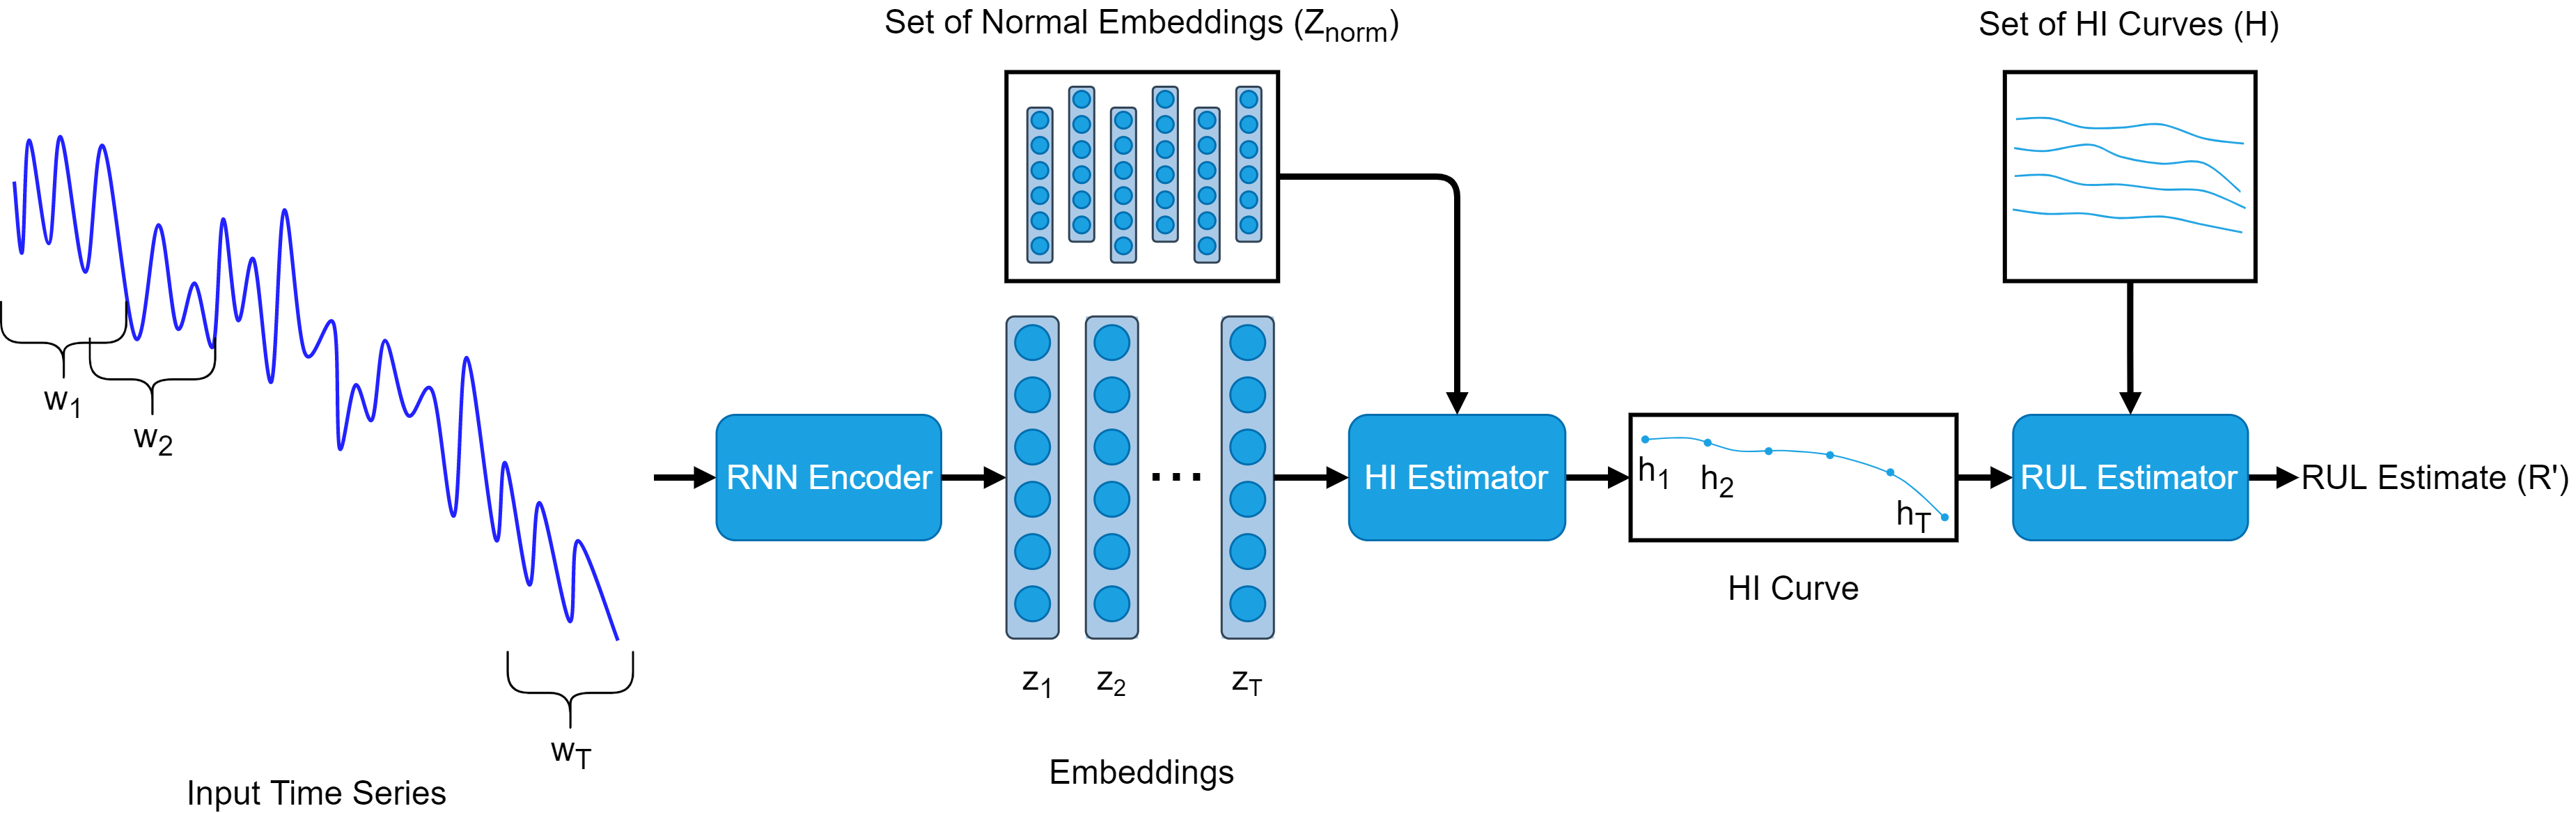
\includegraphics[width=\textwidth]{gfx/rul_embed_rul_pipeline.drawio}
    \caption{Embed-RUL pipeline \cite{DBLP:journals/corr/abs-1709-01073}.}
    \label{fig:embed_rul}
\end{figure}

The pipeline has three different stages that take the raw time series data, transform it into different intermediate representations and generate a RUL estimation in the end. These three stages are described in the following paragraphs.

\subsubsection*{RNN Encoder Decoder Learning}
\label{sec:rul_estimation:approaches:embed_rul:rnn_encoder_decoder_learning}

The time series data is first divided into windows of length $w\in \mathbb{N}$ with maximum overlap (i.e. to create the next window just add the next more recent value and remove the oldest value). The goal of this first step is then to create an embedding $z_i^{(t)} \in \mathbb{R}^c$ (where $c$ is the total number of recurrent units in the RNN Encoder) that serves as a short representation of the time series data in this window.\\
The RNN Encoder Decoder is then trained to obtain functions $f_\text{enc}$ and $f_\text{dec}$ like the following:
\begin{equation}
    \begin{aligned}
        \text{Generate embedding: } z_i^{(t)} = f_\text{enc}(x_i^{(t - w + 1, t)}) \\
        \text{Reconstruct time series: } \widetilde{x}_i^{(t - w + 1, t)} = f_\text{dec}(z_i^{(t)})
    \end{aligned}
\end{equation}
The reconstruction error for training the RNN Encoder Decoder is then given by:
\begin{equation}
    e_i^{(t)} = \sum_{j=(t-w+1)}^t ||x_i^{(j)}-\widetilde{x}_i^{(j)}||^2
\end{equation}
The RNN-ED is then trained to minimize the loss function that sums up the reconstruction error for all windows of time series data and all training set instances where $T\in \mathbb{N}$ denotes the last time step for the training instance:
\begin{equation}
    \mathcal{L} = \sum_{i=1}^N \sum_{t=w}^T e_i^{(t)}
\end{equation}
This provides us with a very robust RNN Encoder that generates a condensed representation of the time series data for use in the next stage.

\subsubsection*{HI Estimator}
\label{sec:rul_estimation:approaches:embed_rul:hi_estimator}

The generated embeddings $z_i^{(w)}, \ldots, z_i^{(T)}$ are then used to perform a health index estimation. The individual embeddings are compared to the embeddings of a normal operation which are maintained in a set $Z_{norm}$. The health index is then achieved as follows:
\begin{equation}
    h_i^{(t)} = min(||z_i^{(t)} - z||) \quad \forall z \in Z_{norm}
\end{equation}
In this notation a low value means a good health because it is close to the normal operation. However this result can be inverted and normalized to obtain a classical health index estimation where 0 means bad and 1 means good health. A health index curve is then denoted like follows:
\begin{equation}
    h_i = \{h_i^{(w)}, h_i^{(w+1)}, \ldots, h_i^{(T)}\}
\end{equation}

\subsubsection*{RUL Estimator}
\label{sec:rul_estimation:approaches:embed_rul:rul_estimator}

The RUL estimation is generated by comparing the HI curve $h_{i^*}$ for a test instance $i^*$ with the HI curves in the set $H$ that contains normal operation values (see Figure~\ref{fig:embed_rul}). The similarity is expressed by the following formula where $T^{(i^*)}$ denotes the last recorded time step for the test instance:
\begin{equation}
    s(i^*, i, t_D) = \exp \left(-\frac{1}{T^{(i^*)}}\sum_{k=w}^{T^{(i^*)}}\left(h_{i^*}^{(k)}-h_i^{(k+t_D)}\right)^2/\lambda\right)
\end{equation}
$\lambda > 0,\ \  t_D\in \{1,2,\ldots,\tau\},\ \  t_D+T^{(i^*)}\leq T^{(i)}$ where $\tau$ denotes the maximum allowed time lag $t_D$ and $\lambda$ scales the term to control how close two health curves have to be. The final RUL is then given by a weighted average using all combinations of $i$ and $t_D$ that satisfy the constraints $s(i^*, i, t_D)\geq\alpha\cdot s_{max}$, where $s_{max}=\max_{0\leq i\leq N, t_D\in \{1,\ldots \tau\}}\{s(i^*, i, t_D)\},\ \  0\leq \alpha\leq 1$. This results in the following formula for the RUL estimate:
\begin{equation}
    R_{i^*} = \frac{\sum s(i^*, i, t_D)\cdot (T^{(i)}-T^{(i^*)}-t_D)}{\sum s(i^*, i, t_D)}
\end{equation}

\subsection{Direct RUL using SVR}
\vspace*{-12.5mm}\hfill{\fontfamily{phv}\normalsize\emph{Vinay Kaundinya}}
\label{sec:rul_estimation:approaches:direct_rul}

%Approaches for RUL estimation have been broadly classified into 3, Model based, Data driven and Hybrid. Model based approaches require specific domain knowledge in building physical models and hence its applicability decreases. Data driven models use statistical learning methods in approximating the system's behavior, based on regularly collected past data. Use of such approaches can offer a tradeoff between precision and applicability. Hybrid approaches are a combination of specific domain knowledge and collected system data.

Most RUL estimation approaches proposed in the literature, have been two stepped. The first step deals with the estimation of health state of the machine and followed by a simple calculation of RUL. However the method proposed in \cite{DBLP:journals/tie/KhelifCMLFZ17} , "\textit{Direct RUL using Support Vector Regression}" is able to estimate RUL without estimating the health states, but directly using the collected sensor data.
\begin{figure}[ht]
    \centering
    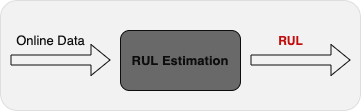
\includegraphics[width=0.5\textwidth]{gfx/rul_direct_rul}
    \caption{Direct RUL estimation \cite{DBLP:journals/tie/KhelifCMLFZ17}}
    \label{fig:direct_rul}
\end{figure}

For Direct RUL approach to take the denoised sensory data as input and output the RUL value, the approach needs to extract the required senor features that can help in associating it to the RUL value. A wrapper method is then used to optimize the number of sensors observed, only the relevant sensor data is taken and the other sensors' data is ignored. This method can be realized in the following 4 steps:

\textit{1: Data sensor selection}: Here the wrapper method is used to select the most relevant sensors.\\
We understand that with any dataset, there exists a good percentage of irrelevant or redundant information and training a model with everything can lead to inaccurate results. Hence it is necessary to filter only relevant information in developing a robust model. Broadly feature selection approaches can be classified into filters, wrappers and embedded methods.
Here we choose wrapper methods, where selection criterion is dependent on the performance of the mining algorithm. This is known to be a time consuming process and hence it is done as a offline process with data only for 5 sensors.

\textit{2: Training set construction}: Here we construct the training set mapping features and their RUL values.\\
First step is to decompose the time series $T_{i}$ into non overlapping windows of size \textit{L}. One of the windows in the time series $T_{i}$, \textit{k}th window can be shown to contain $t^{i}_{(k-1),L+1},,,t^{i}_{kL}$ \cite{DBLP:journals/tie/KhelifCMLFZ17}.
We extract two parameters per dimension, average value \textit{a} and regression trend coefficient \textit{s} for each window. When \textit{d} is the dimensions of the time series $T_{i}$, a feature vector of size \textit{2 X d} is computed. Remaining useful lifetime value can be calculated as follows $$l(T_i) - kL$$
Each vector is then associated with a Remaining useful lifetime value to give us the training set $$D_\text{train} = \{x_i, y_i\}_{i=1}^{N}$$ where \textit{$x_i$}$\in R^{2d}$ and \textit{$y_i$} is the RUL value of the window from its last instant. Here the RUL value is also added to priorly defined $D_\text{train}$.
\begin{figure}[ht]
    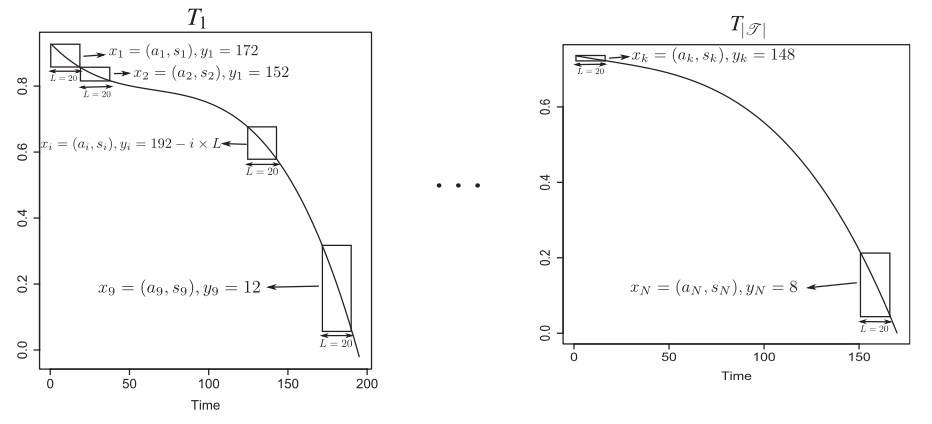
\includegraphics[width=\textwidth]{gfx/rul_trendfeats}
    \caption{An example of windowing technique, $L = 20$, $l(T_{1}) = 192$. \cite{DBLP:journals/tie/KhelifCMLFZ17}}
    \label{fig:trendfeats_rul}
\end{figure}

\textit{3: Learning an SVR model}: We train the SVR model with our training data with relationships between predictor and target variables.\\
In this step, we use the predictor variables $x$ to predict the target variable $y$ using regression technique. We use SVR to model the relationships between predictor and target variables.
$\nu$ SVR and $\epsilon$ SVR are the two types of SVR. Looking at minimizing the error, $\epsilon$ SVR is chosen where parameter $\epsilon$ controls the amount of error allowed in the model. $\epsilon$ SVR looks to work on minimizing $\mid \mid \omega \mid \mid^{2}$ such that,
$$
    \begin{cases}
        y_{i} - \langle \omega,x_{i} \rangle - b \leq \epsilon \\
        \langle \omega,x_{i} \rangle + b - y_{i} \leq \epsilon
    \end{cases}
$$
where $\big \langle .,. \big \rangle$ is the dot product and $\omega$ is the separating plane in a high dimensional space ($\Re^{2d}$). The above conditions might not always satisfy $\epsilon$ margin condition, hence new slack variables $\zeta_{i}$ and $\zeta_{i}^{*}$ are introduced. As in SVM, the kernel trick is used where the input data are mapped into a feature space. The $\epsilon$ SVR is then used to model the non-linear relationships between $x$ and $y$. This is nothing but the model $m$ that can help us find the RUL of components.

\textit{4: Prediction of RUL}: Here we predict the RUL values for the test data.\\
SVR trained as described above is now used to predict the RUL values. Here the model uses the time series $U = \{u_{i}\}_{i = 1}^{l(U)}$. This model aims to predict the time difference between $l(U)$ and the time at which the failure occurs.
In this step we split the time series into windows of size L. A new window($n_{U}$) is obtained by shifting the previous one by one time unit, i.e $n_{U} = l(U) - L + 1$. From each of these $U$ windows a $2d$ feature vector is obtained by extracting the trend features as explained in steps above.

If $x_{k}$ is the feature vector of the $k$th window in the time series, $x_{k}$ is passed to the SVR model $m$ which predicts $y_{k}$, the time at which the failure is supposed to occur. The time is calculated using $\hat{f}_{k} = L + k - 1 + y_{k}$. This will lead to $n_{U}$ such predictions and an average or weighted average of these values gives us the final RUL value of the time series.

\subsection{Random Forests}
\vspace*{-12.5mm}\hfill{\fontfamily{phv}\normalsize\emph{Christopher Zinda}}
\label{sec:rul_estimation:approaches:random_forests}

Random Forests were successfully applied to predict the remaining time until a product becomes obsolete \cite{GSCH:jennings2016forecasting}. It has also been shown that the RUL prediction using Random Forests achieves very low root mean squared error values when compared to other conventional machine learning algorithms \cite{GSCH:mathew2017prediction}. This is why we included the approach in this survey and we will describe it in greater detail in the following section. The explanation of Random Forests is mainly based on the paper by Cutler et al. \cite{GSCH:cutler2012random}.

The approach uses a number of different decision trees and averages their predictions to get a final RUL prediction. From the two available tree types (classification and regression) we are using regression trees because they fit the PdM problem domain. The main issue of decision trees however is that they can be inaccurate and prone to overfitting. This is why multiple regression trees are used and their predictions are averaged.\\
regression trees are binary trees that divide the instances of sensor data into multiple partitions. In Figure~\ref{fig:decision_tree_rul} you can see an example with fictional values. Three sensors were recorded (temp, energy\_use, oil\_pressure) and based on their specific values the decision tree makes a prediction of the RUL. The RUL is denoted in days at the leaf nodes.
\begin{figure}[ht]
    \centering
    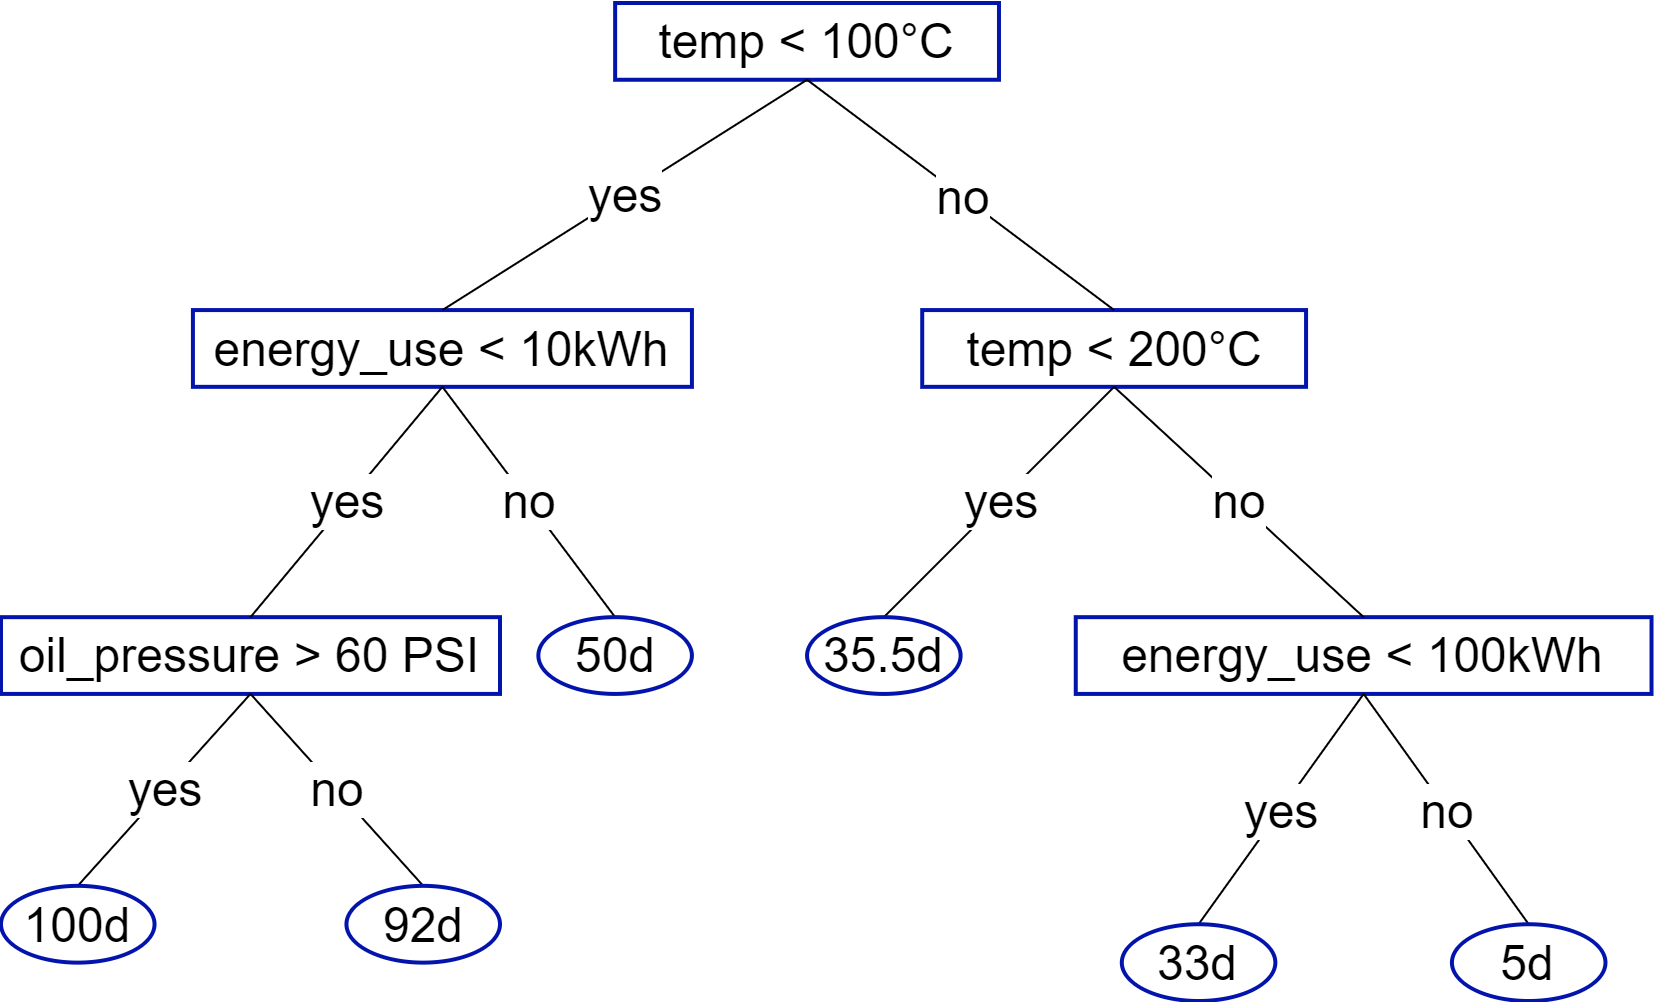
\includegraphics[width=0.8\textwidth]{gfx/rul_decision_tree.drawio}
    \caption{Example of a decision tree for RUL estimation with fictional values.}
    \label{fig:decision_tree_rul}
\end{figure}

A single regression tree is trained by using Binary Recursive Partitioning (BRP). The training set for this algorithm is constructed as follows.
\begin{equation} \label{eq:rul_random_forests_training_set}
    D_\text{train} = \{(x_1, y_1), \ldots, (x_P, y_P)\} \text{ with } x_i = (v_{i,1}, \ldots, v_{i,S})^T
\end{equation}
where $P$ is the total count of all time steps for the $N$ maintenance cycles (i.e. the overall count of sensor readings) and $y_i$ denotes the RUL at the point in time when the sensor values $x_i$ were recorded.\\
The algorithm starts with all training set instances $(x_i, y_i)$ in the root node and searches for the best split among all $S$ sensors. To find the best split, all possible values $v_{i, j}$ for a fixed sensor $j$ are sorted and a split between every distinct pair of values is considered. The threshold of a split is denoted by $c\in \mathbb{R}$ which means that all instances $x_i$ where $v_{i,j} < c$ will be propagated to the left subtree. The remaining instances will be propagated to the right tree. For all values of $c$ and all sensors $j\in [S]$ the score of the split $Q_\text{split}$ is evaluated.
\begin{equation}
    Q_\text{split} = n_LQ_L+n_RQ_R
\end{equation}
where $n_L$ and $n_R$ denote the number of instances that are assigned to the left and right subtree. $Q_L$ and $Q_R$ are evaluated by computing $\frac{1}{n}\sum_{i=1}^n(y_i-\overline{y})^2$ for the left and right subtree. $\overline{y}$ is the average of all labels $y_i$ for the respective subtree which means that $Q_L$ and $Q_R$ can be seen as a measure of similarity. Finally, the split is chosen that minimizes $Q_\text{split}$ and the algorithm works on the two resulting subtrees recursively. The recursion is stopped once a stopping criterion is met and there is no point in further partitioning the data. The stopping criterion could be a smallest number of instances in a leaf node or a maximum number of leaf nodes.\\
Once the training is finished we can use the regression tree to get a RUL prediction for a test instance $x_{i^*}$ by propagating it through the tree based on the recorded sensor values and split thresholds. When a leaf node $k$ is reached, the RUL estimate is computed by taking the average over all labels $y_{k_i}$ of the training data associated with that node.
\begin{equation}
    \hat{h}(x_{i^*}) = \frac{1}{n}\sum_{i=1}^n y_{k_i}
\end{equation}
As described before it is not sufficient to use only a single decision tree. Instead we want to use multiple trees that are trained differently and average over their predictions to get a robust RUL prediction.\\
Let $J$ denote the number of trees that will be trained by the Random Forests algorithm. First the algorithm will obtain a bootstrap sample $D_j$ of size $P$ from the original training set. A bootstrap sample is generated by randomly picking a number of training set instances. After one iteration the instances are placed back in the training set and new instances are randomly selected which opens the possibility for duplicates in the bootstrapped sample set. After the bootstrapping is finished, a regression tree will be trained on that sample, but with a modification to the Binary Recursive Partition algorithm. Instead of searching for a best split on all $S$ sensors, the BRP algorithm will only search on a random selection of $m < S$ sensors.\\
The bootstrapping of the training set and the random selection of sensors ensure a high randomization for the different decision trees. Once all $J$ trees have been trained that way, we can get a robust RUL prediction by averaging over all trees:
\begin{equation}
    R_{i^*} = \frac{1}{J}\sum_{j=1}^J \hat{h}_j(x_{i^*})
\end{equation}

After it was described how the Random Forests algorithm works, we will take a look at the parameters of the approach. There are three parameters which are subject to optimization: $m$ (number of randomly selected sensors), $J$ (number of trees) and the stopping criterion. Usually the default selection for $m$ is $P/3$ and there is no need to do much fine-tuning because overfitting effects due to $m$ are very low. The selection of $J$ however worsens the generalization error if it is chosen too low. $J$ should be selected rather high to get to the point where the generalization error converges. This can be ensured by plotting the Out-Of-Bag (OOB) error for some values of $J$. The OOB error can be computed for the training set instances that were not taken during bootstrap sampling. Lastly, the original work on Random Forests suggests to use a stopping criterion that allows for very large decision trees \cite{GSCH:cutler2012random}. It has to be considered that a large tree size can cause overfitting and the stopping criterion has to be adapted to prevent this.

Random forests have a number of advantages that make them appealing. As shown above, Random Forests only have a few parameters that need to be tuned. Also they have a built-in estimate of the generalization error by computing the OOB error. Lastly, they can be implemented in parallel which makes the training relatively fast. To conclude, Random Forests provide a powerful tool for predicting the RUL of a machine.

\subsection{CNN based Regressor}
\vspace*{-12.5mm}\hfill{\fontfamily{phv}\normalsize\emph{Vinay Kaundinya}}
\label{sec:rul_estimation:approaches:cnn_rul}

Estimation of remaining useful lifetime of a component or a subsystem becomes crucial in varied application areas like manufacturing, aerospace etc. Existing algorithms in predicting RUL of a component are all based on multivariate analysis or damage progression analysis. To accurately predict RUL becomes challenging if there is no good representation of features. In the paper \cite{DBLP:conf/dasfaa/BabuZL16}, the authors Giduthuri Sateesh Babu, Peilin Zhao, and Xiaoli Li  proposed an approach that estimates RUL as a multivariate time series regression task based on Convolutional Neural Network(CNN), adapted from deep learning techniques for image classification.

As part of the approach, a sliding window strategy is adopted to segment the multivariate time series data into short segments of signals. These signals($r$) along with their attributes($D$) then form a 2 dimensional  matrix ($r \times D$), which forms as an instance of input to CNN. In case of single operating condition, the raw signals($d$) becomes the input. However in case of multiple operating conditions dataset, raw sensor signals and the features attributed to operating conditions are included. Here, we use 2 pairs of convolution layers and pooling layers and finally connected to a multi layered perceptron for RUL estimation. In CNN, $r$ (windowing rate or sampling rate) is chosen to be 15 and step size of 1. First we feed the segmented multivariate time series($D \times 15$) as input through 2 layers of convolution and pooling layers. Then all the feature maps are concatenated at the end of the last pooling layer into a vector input for MLP for RUL estimation.
\begin{figure}[ht]
    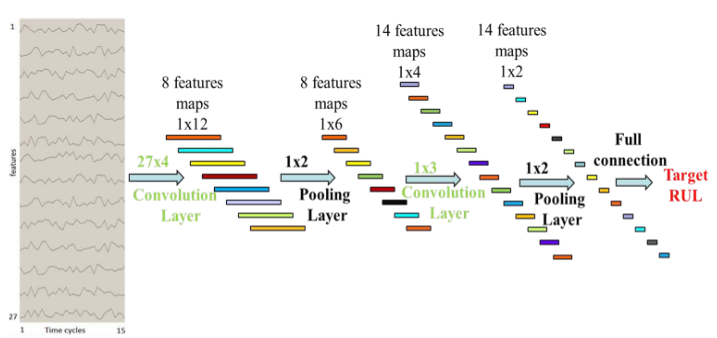
\includegraphics[width=\textwidth]{gfx/rul_cnn_architecture}
    \caption{CNN architecture proposed to estimate RUL. It includes 2 pairs of convolution and pooling layers and a fully connected MLP layer. \cite{DBLP:conf/dasfaa/BabuZL16}}
    \label{fig:cnn_archi_rul}
\end{figure}

In convolution layers, the input from the previous layer is convolved using a kernel that is learned during training. Then the activation function computes the next layer feature maps,
\begin{equation}
    x_{j}^{l} = sig(z_{j}^{l}),    z_{j}^{l} = \sum_{i}x_{i}^{l-1} * k_{ij}^{l} + b^{l}_{j}
\end{equation}
Here, * is the convolution operator, $x_{i}^{l-1}$ and $x_{j}^{l}$ are the input and output of the convolutional layer and $sig()$ denotes the sigmoid function. We apply first convolution filter of size $D \times 4$ in the first layer and of size $1 \times 3$ in the second layer.

In pooling layers, features output from the convolution layer is then segmented or sub-sampled into set of non overlapping data, to increase the invariance of features to distortions on the inputs. Here we use the average pooling, to get the average value of the sub-samples as its output.
\begin{equation}
    x_{j}^{l+1} = down(x_{j}^{l})
\end{equation}
where, $x_{j}^{l}$ is the input to the pooling layer and $x_{j}^{l+1}$ is the output. $down()$ acts as the sub-sampling function for average pooling. The size of both the pooling layers is $1 \times 2$.

In training the proposed CNN approach, we use the squared error loss function and the procedure consists of phases of forward propagation, backward propagation and the application of gradients. The loss function is defined as follows:
\begin{equation}
    E = 1/2(y(t) - y^{*}(t))^2
\end{equation}
where $y(t)$ is the target RUL and $y^{*}(t)$ is the predicted RUL value.

\textbf{Forward propagation} deals with computing output feature maps of each layer and also the output of CNN model as whole. The outputs of the convolution and pooling layers are computed using equations 5.11 and 5.12 respectively. These outputs are then fed into a single fully connected layer.
Once after an iteration of forward propagation, the error value after squared error loss function is available. \textbf{Backward propagation} is initiated and deals with error value and propagates from the last layer to first. As the errors propagate from last layer to first, derivatives are calculated using following functions,

$up()$: This function has an inverse operation of the $down$ function as defined above. \\
$reverse()$: This reverses the function of feature extractors. \\
$pad()$: Adds zeroes as padding, as described in the paper \cite{DBLP:conf/dasfaa/BabuZL16}.

Once we get the values of parameter derivatives we apply them to update the parameters. If $E(w)$ is the cost function that we try to minimize, then \textbf{Gradient} descent suggest to modify the values in the direction of its steepest descent, such that
\begin{equation}
    w^{l}_{ij} = w^{l}_{ij} - \eta \frac{\delta{E}}{\delta{w^{l}_{ij}} }
\end{equation}
Here $w_{ij}$ is the weight to be modified and $\eta$ is the learning rate that will determine how much modification the weight will have. Larger the $\eta$, greater the modification of $\omega_{ij}$.

\subsection{Multiple Classifier Approach}
\vspace*{-12.5mm}\hfill{\fontfamily{phv}\normalsize\emph{Christopher Zinda}}
\label{sec:rul_estimation:approaches:multiple_classifier_approach}

The Multiple Classifier Approach as described in the paper by Susto et al. trains multiple classification modules with different prediction horizons to gain information about the best time to do maintenance with minimal costs \cite{DBLP:journals/tii/SustoSPMB15}. The following chapter therefore describes the findings of that paper to provide you with an insight in this different approach and shows how it can be applied to the prediction of RUL.

The training set for the approach is defined like in equation~\ref{eq:rul_random_forests_training_set} where $P$ is the total count of all time steps for the $N$ maintenance cycles (i.e. the overall count of sensor readings), but $y_i$ has a different meaning. If there was a breakdown of the machine at time step $i\in[P]$, then the label is \textit{faulty} (F). Otherwise it is \textit{not faulty} (NF):
\begin{equation}
    y_i = Y(i) = \begin{cases}
        \text{F,}  & \text{if iteration }i\text{ is faulty}     \\
        \text{NF,} & \text{if iteration }i\text{ is not faulty}
    \end{cases}
\end{equation}
However, this would cause the dataset to be very unbalanced and skewed. With the current definition there are $N$ faulty instances and $P-N$ instances that are not faulty. Typically $P\gg N$ which results in an unbalanced training set and will cause poor prediction accuracy and generalization.\\
To mitigate this issue, the Multiple Classifier Approach trains several classifiers on training sets with varying failure horizon $m\in\mathbb{N}$. The failure horizon defines the number of instances at the end of a maintenance cycle that will be marked as faulty:
\begin{equation}
    y_i^{(t)} = \begin{cases}
        \text{F,}  & \text{if }t > n_i - m_j \\
        \text{NF,} & \text{otherwise}
    \end{cases}
\end{equation}
where $t$ is the time step in the $i$th maintenance cycle which has length $n_i$ and $m_j$ denotes the failure horizon for the $j$th classifier.\\
The type of classifier can be chosen independently. In the cited paper they are using k-NN which is a simple classifier and SVM which yields slightly better results.

The approach that is suggested in the paper by Susto et al. uses a training and an additional validation set to perform crossvalidation \cite{DBLP:journals/tii/SustoSPMB15}. They are obtained by randomly splitting the maintenance cycles using a factor $0 < q < 1$ such that $N_\text{train} = \lfloor Nq\rfloor$ and $N_{val} = \lceil N(1-q)\rceil$.\\
To train a single classifier, the algorithm first executes a number of $Q$ simulations to tune the hyperparameters. In every simulation random training and test sets are obtained using the factor $q$. The misclassification rate (MCR) is then evaluated for different hyperparameters. Based on these results, the hyperparameters are chosen that had the lowest average MCR over all simulations. This whole process is repeated for each of the $J$ classifiers using their specific failure horizon $m_j$. The failure horizon for the $j$th classifier should be set to $m_j = j$. This results in $J$ trained and fine-tuned classifiers that can be used to predict the RUL.

Because we trained the classifiers in a way that the $j$th one learns to predict a failure when there are less than or equal to $j$ time steps left (failure horizon $m_j = j$), we can obtain the actual RUL prediction by finding the lowest index $j^*$ such that all classifiers with index $j \geq j^*$ predict F.
\begin{equation}
    R_{i^*} = \min j^* \::\: \hat{h}_j(x_{i^*}) = \text{F},\quad \forall j \geq j^*
\end{equation}
where $\hat{h}_j$ is the output of the $j$th classifier.

\subsection{Long Short-Term Memory}
\vspace*{-12.5mm}\hfill{\fontfamily{phv}\normalsize\emph{Vinay Kaundinya}}
\label{sec:rul_estimation:approaches:lstm_rul}

From the different approaches we have described above, we can say that regression based and neural network based models extract features from the segmented windows of the time series data. However, these techniques face issues in accurately modelling long term dependencies and when modelling sequence information. We now describe a Long Short Term Memory (LSTM) approach for RUL estimation as proposed in the paper \cite{DBLP:conf/icphm/ZhengRFG17} by the authors Shuai Zheng, Kosta Ristovski, Ahmed K Farahat, and Chetan Gupta. This approach looks at making full use of the sensor data in extracting the required feature information, leveraging multiple layers of LSTM cells.

According to definition $\mid s\mid$ is the number of sensors, here a $\mid s\mid$-dimensional time series data is passed as input to the $LSTM$ model and $y$ as estimated RUL value is the output. The proposed model is consists of multiple layers of LSTM cells followed by a feed forward neural networks(NN). Each LSTM layer is then made up of sequence of LSTM cells. A typical LSTM model looks as shown in figure \ref{fig:lstm_rul}.
\begin{figure}[ht]
    \centering
    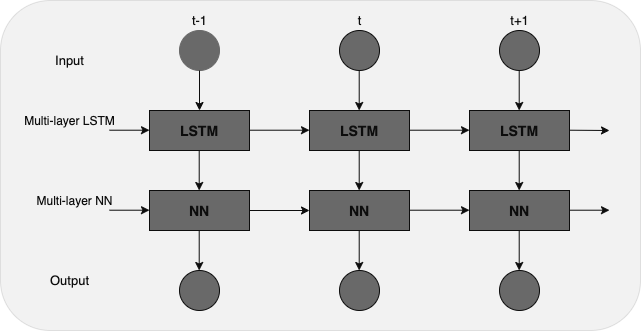
\includegraphics[width=0.7\textwidth]{gfx/rul_lstm1}
    \caption{LSTM Model. \cite{DBLP:conf/icphm/ZhengRFG17} }
    \label{fig:lstm_rul}
\end{figure}

Output of an LSTM cell is a value $h^t$ and also its state $c^t$, both of which are vectors of the same size at time instant $t$. Size of these vectors are defined by the number of nodes($m$) a cell contains. As each layer is a sequence of such cells, the output($h^{t-1}$) and state($c^{t-1}$) of a LSTM cell at time $t-1$ becomes the input for the next LSTM cell at time $t$. Each cell consists of 3 gates: input gate($i^t$), output gate($o^t$) and forget gate($f^t$). Input gate controls the information that will be passed on from the previous cell $h^t$ and the time series input data $x^t$. Output gate controls what will be passed on to the next cell. Forget gate is responsible for controlling information what a cell will retain as memory.

In the proposed approach, different variable weights and biases that will be computed during the training process in each cell are denoted by $W$, $U$ and $b$. $\sigma$ denotes the sigmoid activation function and a hyperbolic function $tanh$ is used in LSTM cells of this model. Each cell implements the following in the proposed model,
\begin{equation}
    i^t = \sigma(W_ix^t + U_ih^{t-1} + b_i)
\end{equation}
\begin{equation}
    o^t = \sigma(W_ox^t + U_oh^{t-1} + b_o)
\end{equation}
\begin{equation}
    f^t = \sigma(W_fx^t + U_fh^{t-1} + b_f)
\end{equation}
\begin{equation}
    a^t = tanh(W_cx^t + U_ch^{t-1} + b_c)
\end{equation}
\begin{equation}
    c^t = f^t \odot c^{t-1} + i^t \odot a^t
\end{equation}
\begin{equation}
    h^t = o^t \odot tanh(c^t)
\end{equation}
$\odot$ denotes element wise multiplication of 2 vectors. The internal structure of LSTM cell that is used here to estimate RUL for a component,
\begin{figure}[ht]
    \centering
    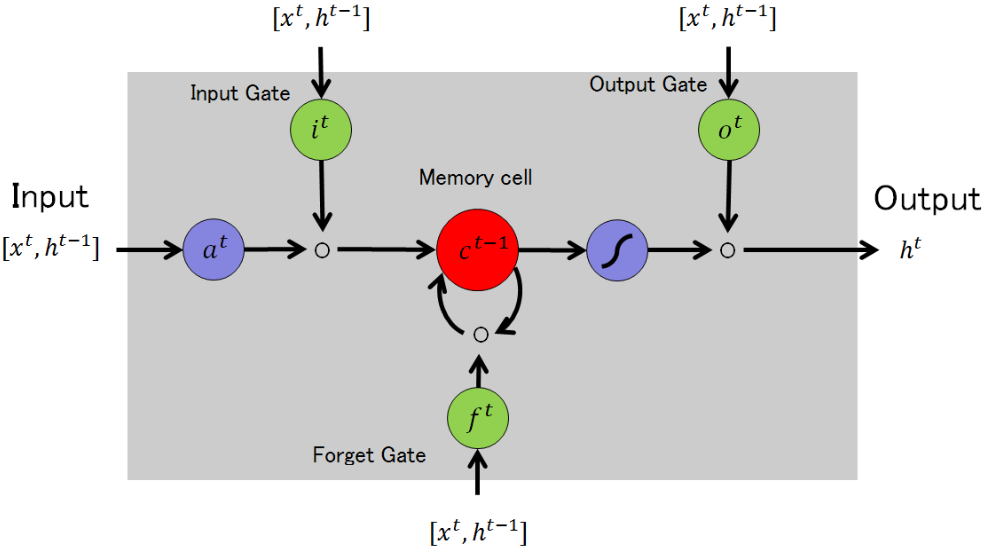
\includegraphics[width=0.7\textwidth]{gfx/rul_lstm2}
    \caption{LSTM Cell in the proposed model. \cite{DBLP:conf/icphm/ZhengRFG17} }
    \label{fig:lstm2_rul}
\end{figure}

RMSprop optimizer is used to train the model and use dropout to control overfitting. This model also aims to optimize the error function with respect to above defined variable weights and biases. The error function is given by the ,
\begin{equation}
    E = \sum_{i=1}^{t} \mid \mid y_i - \hat{y_i} \mid \mid^2
\end{equation}
Different types of sensors are used and the value scale for each of those also vary, this calls for normalization of sensor data before it is used for training or testing. Two normalizations, \textbf{z-score} normalization and \textbf{min-max} normalization are applied to the data,\\
\textbf{z-score normalization}
\begin{equation}
    x_i^\prime = \frac{x_i - \mu_i}{\sigma_i}
\end{equation}
\textbf{min-max normalization}
\begin{equation}
    x_i^\prime = \frac{x_i - min(x_i)}{max(x_i)-min(x_i)}
\end{equation}
Proposed structure is adequate for RUL estimation due to the fact that this LSTM approach \cite{DBLP:conf/icphm/ZhengRFG17} utilizes the complementarity modeling capability of LSTM and NN. LSTM is responsible for temporal modeling. NN is good at mapping LSTM feature to regression outcomes.

\section{Evaluation Setup}
\vspace*{-12.5mm}\hfill{\fontfamily{phv}\normalsize\emph{Vinay Kaundinya}}
\label{sec:rul_estimation:evaluation_setup}

To compare performance of a different models, we need to define few objective performance measures. Looking into the approaches described above, we employ the following symmetric and asymmetric functions as part of performance measures

\subsection{Symmetric Loss Functions}
\label{sec:rul_estimation:evaluation_setup:sym_loss}

\subsubsection*{RMSE}

Root Mean Squared Error(RMSE) is chosen as one of the performance measures in predicting RUL. This is a symmetric function, which penalizes both early and late predictions by giving them equal weights. We define RMSE in equation \ref{rmse:eq1},
\begin{equation} \label{rmse:eq1}
    RMSE = \sqrt{\frac{1}{N}\sum^{N}_{i=1}(y_{i} - \hat{y_{i}})^2}
\end{equation}
Here, $N$ is the total number of cycles in the time series and $y_{i} - \hat{y_{i}}$ is the difference between the predicted RUL value and the actual RUL value. We look at the RMSE values for each approach and the approach with lower RMSE value is chosen as a better approach.

\subsubsection*{MAPE}

Mean Absolute Percentage Error(MAPE) is the other chosen performance measure which is also symmetric in nature. MAPE is nothing but the mean or average of the absolute difference of predicted and actual RUL values, expressed in percentages.
\begin{equation}
    MAPE = \frac{100}{N}\sum^{N}_{i=1}\frac{\mid y_{i} - \hat{y_{i}} \mid}{\hat{y_{i}}}
\end{equation}
Here, $y_{i}$ is the predicted RUL value and $\hat{y_{i}}$ is the actual RUL value. MAPE values are percentages and hence makes it easier to compare Error percentages of different approaches. Approach with smaller MAPE is the better approach.

\subsection{Asymmetric Loss Functions}
\label{sec:rul_estimation:evaluation_setup:asym_loss}
We know that neural networks aim to minimize the errors by adjusting weights in each layer so that the correct mapping of input to output happens, during the training process. Symmetric loss functions might fall short in penalizing cases where early prediction and late prediction do not have the same effect, specially here in our case of estimating RUL for a component. Hence, we define a few asymmetric loss functions in this section, that can be used to penalize an early prediction differently from a late prediction.
\subsubsection*{LIN-LIN}
Given a test dataset and a model to predict, we can easily compute the absolute error loss by finding an absolute difference between the actual RUL $\hat{y_{i}}$ and the predicted RUL $y_{i}$ values. Absolute error loss function $f_{AE}$ defined in equation \ref{lin:eq2} is a symmetric function.
\begin{equation} . \label{lin:eq2}
    f_{AE}(\hat{y_{i}},y_{i}) = \mid \hat{y_{i}} - y_{i} \mid
\end{equation}
In order to convert this loss function into an asymmetric loss function, we then introduce weights $a$ and $b$ which will be multiplied to the loss function. Now we get a function (\ref{lin:eq1}), which incase of $a \neq b$ becomes an asymmetric loss function, known as $LIN-LIN$ asymmetric loss function.
\begin{equation} \label{lin:eq1}
    f_{LIN-LIN}(a, b,\hat{y_{i}},y_{i}) = \begin{cases}
        -a(\hat{y_{i}} - y_{i}),\hspace{1cm}if \hat{y_{i}} - y_{i} \leq 0 \\
        b(\hat{y_{i}} - y_{i}),\hspace{1cm}otherwise
    \end{cases}
\end{equation}

\subsubsection*{Score}

We define another loss function called $Score$ function ($S$) as an important objective performance measure,
\begin{equation}
    S = \begin{cases}
        \sum^{N}_{i=1}(e^{-\frac{y_i-\hat{y_i}}{13}}-1),\hspace{1cm} if y_i - \hat{y_i} < 0 \\
        \sum^{N}_{i=1}(e^{\frac{y_i-\hat{y_i}}{10}}-1),\hspace{1cm} if y_i - \hat{y_i} \geq 0
    \end{cases}
\end{equation}
Here, the late predictions or cases where its too late to perform maintenance are penalized more than the early predictions. In case of early prediction, one has enough time to perform maintenance. The lower the Score function value the better is the approach or model being tested.

\subsubsection*{Performance}

We also introduce another metric that evaluates the overall algorithm accuracy called Performance. According to this metric all prediction values must be within an acceptable range to be considered as correct prediction. The acceptable range is $[-10, 13]$. This provides a percentage of correct predictions, whereas $score$ gives us an idea of the overall error.  % INCLUDE: remaining useful lifetime estimation
% !TEX root = ../main.tex
%
\chapter{Conclusion}
\vspace*{-15mm}
\hfill{\fontfamily{phv}\normalsize\emph{Christopher Zinda, Gourav Prakash, Paul Fährmann and Vinay Kaundinya}}
\label{sec:conclusion}

\cleanchapterquote{Prediction is very difficult, especially if it's about the future.}{Nils Bohr}{(Physicist)}

In this survey, we presented and connected three different problems of data-driven Predictive Maintenance: Health State Classification, Health Index Estimation and Remaining Useful Lifetime Estimation. We gave a structured overview of various machine learning models and data sets for those problems and adapted the formal notations of these methods. Also, we researched and presented some feature extraction methods for multivariate time series data.

\subsection*{Pipeline}

The different methods and models presented in this survey are connected in a pipeline setup. We structured the previous chapters along those pipeline elements. Connected through the formal definitions we also advised evaluation setups for each of these pipeline elements in which the collected data sets can be used to evaluate the described methods and models.

\subsection*{Formal definitions}

A common problem when reading and comparing multiple machine learning approaches is that there are always some differences in the understanding of time series and the corresponding formal definition. Therefore we transformed the individual mathematical notations of every paper into one unified standard notation. This way the reader can easily understand new approaches and does not have to learn and adapt multiple different mathematical notations. For this purpose, we also provided a single streamlined definition of time series data in \ref{sec:intro:time-series-definition} which is used throughout the document.


\subsection*{Datasets}

Different state-of-the art approaches were described for each of the three different challenges in PdM, Health State Classification, Health Index Estimation and Remaining Useful Lifetime Estimation. Each of these research approaches can be tested and verified on datasets that were described under Available Datasets sections \ref{sec:HS:datasets}, \ref{sec:hi_estimation:datasets} and \ref{sec:rul_estimation:datasets}. Section \ref{sec:HS:datasets} provides an idea on the two publicly available datasets, condition monitoring of hydraulic systems dataset and bearing fault dataset which is used in demonstrating the classification of Health state of a component or subsystem.

We know that Health Index Classification is one of the techniques used to predict the system state. To validate the approaches of Health Index we use the Milling dataset and Bearing data as described under \ref{sec:hi_estimation:datasets}. In RUL estimation, approaches were used to learn complex dependencies between the different sensors of a component and then obtain RUL of the component. Datasets containing multivariate time series of a aero propulsion system were then described under section \ref{sec:rul_estimation:datasets}.

\subsection*{Future work}

Aside from the approaches mentioned in this survey paper, there are a few approaches and aspects of PdM for ML that need further investigation. Some of the few future works are as follows:


\begin{enumerate}
    \item Digital twins: This is a significant way to achieve smart manufacturing, and it offers a new paradigm for diagnosing faults.The advantage of this method is its saves training time and does not require a lot of data from the target task \cite{DBLP:journals/access/XuSLZ19}.

    \item Generative adversarial network(GAN): A good approach to train a classifier in a semi-supervised way. It does not introduce any deterministic bias compared to auto-encoders. Apart from that, it can be used to address the issue of class imbalance \cite{Goodfellow2014GenerativeAN}.

    \item Predictive maintenance in industry 4.0 is one of the popular systematic approaches which focuses mainly on addressing data analytics and machine learning methods to change production procedures, so not comprising predictive maintenance methods and their organization \cite{DBLP:journals/candie/ZontaCRLTL20}.
\end{enumerate}

However, with the rapid change in technologies where machines are daily confronted with decision making involving a massive input of data and customization in the manufacturing process. The ability to predict the need for maintenance of assets at a specific future moment is one of the main challenges in the Predictive Maintenance for Machine Learning.



                            % INCLUDE: conclusion

% --------------------------
% Back matter
% --------------------------
% \appendix\cleardoublepage
% \input{content/chapter-appendix}       % INCLUDE: appendix
%
{%
    \setstretch{1.1}
    \renewcommand{\bibfont}{\normalfont\small}
    \setlength{\biblabelsep}{0pt}
    \setlength{\bibitemsep}{0.5\baselineskip plus 0.5\baselineskip}
    \printbibliography[nottype=online]
    % \newrefcontext[labelprefix={@}]
    \printbibliography[heading=subbibliography,title={Datasets},type=online]
}
\cleardoublepage
\listoffigures
\cleardoublepage
\listoftables
\cleardoublepage


% !TEX root = ../main.tex
%
\pagestyle{empty}
\hfill
\vfill
\pdfbookmark[0]{Colophon}{Colophon}
\section*{Colophon}

This thesis was typeset with \LaTeXe.
It uses the \textit{Clean Thesis} style developed by Ricardo Langner.
The design of the \textit{Clean Thesis} style is inspired by user guide documents from Apple Inc.

Download the \textit{Clean Thesis} style at \url{http://cleanthesis.der-ric.de/}.

% \cleardoublepage

% \input{content/declaration}
\clearpage
\newpage
\mbox{}

% **************************************************
% End of Document CONTENT
% **************************************************
\end{document}
